\documentclass[10pt]{article}
\input{preamble}

\title{\textbf{Symbolic AI - Definitions and Illustrations}}
\author{Ibrahim Nasser\thanks{This document and its source files are licensed under Creative Commons Attribution--NonCommercial--NoDerivatives 4.0 International License (\href{https://creativecommons.org/licenses/by-nc-nd/4.0/legalcode}{CC BY-NC-ND 4.0}).}}

\date{\small Last updated on \today}

\begin{document}
\pagenumbering{roman}
\maketitle
%\setcounter{tocdepth}{1}
\tableofcontents
\section*{Disclaimer}
This document is an independent summary by \href{https://96ibman.github.io/ibrahim-nasser/}{Ibrahim Nasser} as a personal learning and documentation effort for the courses \href{https://alea.education/FAU/smai/WS25-26}{Symbolic Methods for AI} and \href{https://alea.education/course-home/ai-1}{AI 1: Artificial Intelligence 1} taught by \href{https://kwarc.info/people/mkohlhase/}{Prof. Dr. Michael Kohlhase}.
It is not an official course document, and no guarantee is made for its correctness, completeness, or accuracy.
The material here is meant as an auxiliary resource for understanding the subjects and should not be used as the sole basis for exams preparation. The official lecture notes and course materials remain the authoritative reference.

This summary is a living document, i.e. I may continue to revise, extend, and improve it over time as I refine my understanding or receive feedback.

If you find any mistakes, unclear explanations, or have suggestions for improvement, please \href{mailto:ibrahim.nasser@fau.de}{contact me}.
\clearpage
\pagenumbering{arabic}
\setcounter{page}{1}
\include{intro}
\labeledsection{Mathematical Language}{sec:mathlanguage}
\definition{Natural Language}{
A natural language is any form of spoken or signed means of communication that has evolved naturally in humans through use and repetition without conscious planning or premeditation.
}{natural_language}

\definition{Domain of Discourse}{
The \linkterm{set}{def:set} of entities, objects, or concepts that a language, discussion, or formal system refers to. It specifies the scope within which terms, statements, and reasoning apply.  
}{domain_of_discourse}

\definition{Jargon (Terminology)}{
    A jargon (or terminology) is a \linkterm{set}{def:set} of specialized words or phrases (called technical terms or just terms) relating to concepts from a particular \linkterm{domain of discourse}{domain_of_discourse}.
}{terminology}


\definition{Technical Language}{
A technical language is a \linkterm{natural language}{natural_language} extended by a \linkterm{terminology}{terminology} and (possibly) special idioms, discourse markers, and notations.  
}{technical_language}

\definition{Stylized Language}{
Mathematicians use a stylized language that uses formulae to represent mathematical objects, uses math idioms for special situations (e.g. "iff", "hence", "let... be..., then..."), and classifies statements by role (e.g., definition, Lemma, Theorem, Proof, Example).
}{stylized_language}

\definition{Mathematical Vernacular}{
A \linkterm{technical language}{technical_language} that you need to master to be successful when moving to a new environment (\linkterm{symbolic AI}{symbolicai}).
}{mathematical_vernacular}

\definition{Formulae}{
    A mathematical formula can be a \refterm{mathematical statement}{math_statement} (clause) which can be true or false (e.g. $x>5, 3+5=7$), or a \refterm{mathematical object}{math_object} (e.g. $3, n, x^2 + y^2 + z^2, \int_1^0 x^{3/2} dx$)
}{formulae}

\textbf{Observation: }\linkterm{mathematical vernacular}{mathematical_vernacular} loves to name 
\linkterm{objects}{math_object}/\linkterm{statements}{math_statement} for precise references. For example: Let $p=3x^2+7x$, then $p^3 + 17p + 1 \text{ is } \cdots$

Moreover, \linkterm{mathematical vernacular}{mathematical_vernacular} aggregates \linkterm{objects}{math_object}/\linkterm{statements}{math_statement} for cognitive efficiency, examples:
\begin{itemize}
    \item $a \in S, b \in S, \text{ and } c \in S \leadsto a, b, c \in S$ (\linkterm{object}{math_object} aggregation)
    \item $i \geq 0 \text{ and } i \leq n \leadsto 0 \leq i \leq n$ (\linkterm{statement}{math_statement} aggregation)
\end{itemize}


\definition{Sequence}{
    \linkterm{mathematical vernacular}{mathematical_vernacular} uses the concept of sequences instead of lists. Sequences are usually finite, but can be infinite as well.
}{sequence}

\definition{Ellipses}{
    \linkterm{mathematical vernacular}{mathematical_vernacular} uses ellipses ($\cdots$) as a constructor for \linkterm{sequences}{sequence}. The meaning of an ellipsis is usually considered "obvious" and left for interpretation by the reader.
}{ellipses}

\linkterm{ellipses}{ellipses} allow to write down large \linkterm{objects}{math_object} easily, examples:
\begin{itemize}
    \item $1, \cdots, n \leadsto$ the \linkterm{sequence}{sequence} of natural numbers between 1 and $n$ in order.
    \item $1, 4, 9, 16, \cdots \leadsto$ the \linkterm{sequence}{sequence} of squares in orders.
    \item $e_1, \cdots, e_n \leadsto$ a \linkterm{sequence}{sequence} of \linkterm{objects}{math_object} $e_i$ for $1 \leq i \leq n$
\end{itemize}

\linkterm{Mathematical statements}{math_statement} come in different epistemic varieties:
\begin{itemize}
    \item \refterm{Definitions}{definitions}: \linkterm{statements}{math_statement} that introduce new global identifier for important \linkterm{objects}{math_object}
    \item \refterm{Assertions}{assertions}: \linkterm{statements}{math_statement} that state properties of \linkterm{mathematical objects}{math_object}
    \item \refterm{Examples}{examples}: \linkterm{statements}{math_statement} that exhibit a witness for some property
    \item \refterm{Axioms}{axiom}: \linkterm{statements}{math_statement} that characterize the \linkterm{objects}{math_object} of a certain \linkterm{domain of discourse}{domain_of_discourse} or theory. An axiom (postulate) is a statement about \linkterm{mathematical objects}{math_object} that we \textit{assume} to be true.
\end{itemize}

\linkterm{Mathematical assertions}{assertions} are pragmatically classified into categories:
\begin{itemize}
    \item \refterm{proofs}{proofs} are arguments that justify the truth of \linkterm{statements}{math_statement} beyond any doubt. \linkterm{Proofs}{proofs} are not really \linkterm{statements}{math_statement}, but we sometimes treat them together.
    \item \refterm{proposition}{proposition} is a \linkterm{statement}{math_statement} which is interesting in its own right.
    \item \refterm{lemma}{lemma} is an easily proved \linkterm{statement}{math_statement} which is helpful for proving other \linkterm{propositions}{proposition} and \linkterm{theorems}{theorem}, but is usually not particularly interesting in its own right. A \linkterm{lemma}{lemma} is an intermediate \linkterm{theorem}{theorem} that serves as part of a \linkterm{proof}{proofs} of a larger \linkterm{theorem}{theorem}.
    \item \refterm{theorem}{theorem} is a more important \linkterm{statement}{math_statement} than a \linkterm{proposition}{proposition} which says something definitive on the subject, and often takes more effort to prove than a \linkterm{proposition}{proposition} or \linkterm{lemma}{lemma}. A \linkterm{theorem}{theorem} is a \linkterm{statement}{math_statement} about \linkterm{mathematical object}{math_object} that we \textit{know} to be true.
    \item \refterm{corollary}{corollary} is a quick consequence of a \linkterm{proposition}{proposition} or \linkterm{theorem}{theorem} that was proven rececently. It is a \linkterm{theorem}{theorem} that follows directly from another \linkterm{theorem}{theorem}.
    \item \refterm{conjecture}{conjecture} is a \linkterm{statement}{math_statement} that is thought to be provable, but has not been yet. A \linkterm{conjecture}{conjecture} that is proven is a \linkterm{theorem}{theorem}
\end{itemize}

\linkterm{Mathematical statement}{math_statement} use abbreviations, examples:
\begin{itemize}
    \item $\land$ and $\lor$ for "and" and "or",
    \item $\neg$ for "not"
    \item $\forall x.P \quad (\forall x \in S.P)$ for "condition $P$ holds for all $x$ (in $S$)"
    \item $\exists x.P \quad (\exists x \in S.P)$ for "there exists an $x$ (in $S$) such that the condition $P$ holds"
    \item $\nexists x.P \quad (\nexists x \in S.P)$ for "there exists no $x$ (in $S$) such that the condition $P$ holds"
    \item $\exists^1 x.P (\exists^1 x \in S.P)$ for "there exists one and only $x$ (in $S$) such that the condition $P$ holds"
    \item "\textit{iff}" for "if and only if", symbolized by $\Leftrightarrow$ 
    \item $\Rightarrow$ for "implies"; we can read $A \Rightarrow B$ as "if $A$ then $B$"
\end{itemize}

\definition{Declaration}{
    In \linkterm{mathematical vernacular}{mathematical_vernacular} we call a clause that introduce new identifiers together with some properties a declaration. For example $\text{Let } \epsilon, \delta > 0 \cdots$
}{declaration}

\definition{Scope}{
    The scope of an identifier is the part of an expression where the reference is valid; that is, where the identifier can be used to refer. In the other parts, the identifier may refer to a different entity, or to nothing at all (unbound)
}{scope}

\textbf{Observations:} \linkterm{definition}{definitions} have \textit{global} \linkterm{scope}{scope}, \linkterm{declarations}{declaration} have \textit{local} \linkterm{scope}{scope}.

\definition{Definiendum}{
    The definiendum is the symbol, expression, or term being introduced by a \linkterm{definition}{definitions}. It is the newly named \linkterm{object}{math_object} or concept.
}{defineiendum}

\definition{Definiens}{
    The definiens is the symbol, expression, or construction that specifies the meaning of the \linkterm{defineiendum}{defineiendum}. It explains what the \linkterm{defineiendum}{defineiendum} denotes.
}{definiens}

\linkterm{Mathematics}{mathematics} has developed various forms of \linkterm{definition}{definitions} (definition schemata). A \refterm{simple definition}{simpledefinition} introduces a name (the \linkterm{defineiendum}{defineiendum}) for a compound \linkterm{object}{math_object} or concept (the \linkterm{definiens}{definiens}). The \linkterm{defineiendum}{defineiendum} must be new, i.e. may not have been used for anything else, in particular, the \linkterm{defineiendum}{defineiendum} may not occur in the \linkterm{definiens}{definiens}. We use the symbols $:=$ (and the inverse $=:$) to write \linkterm{simple definitions}{simpledefinition}. For example, we can give the natural number $2$ the name $\phi$. In a \linkterm{formula}{formulae} we write this as $\phi := 2$ or $2 =: \phi$.

On the other hand, in a \refterm{pattern definition}{patterndefinition} the \linkterm{defineiendum}{defineiendum} is the \linkterm{operator}{arithmetic} or \linkterm{relation}{relation} applied to $n$ distinct variables -called pattern variables- $v_1, \cdots, v_n$ as arguments, and the \linkterm{definiens}{definiens} is an expression in these variables. When the new \linkterm{operator}{arithmetic} is applied to arguments $a_1, \cdots, a_n$, then its value is the \linkterm{definiens}{definiens} expression where the $v_i$ are replaced by the $a_i$. We use the symbol $:=$ for \linkterm{operator}{arithmetic} definitions and $:\Leftrightarrow$ for \linkterm{relation}{relation} definitions. For example, the following is a \linkterm{pattern definition}{patterndefinition} for the \linkterm{set intersection operator}{set_intersection} $\cap$:
\[
A \cap B := \set{x \mid x \in A \land x \in B}
\] 
The pattern variables are $A$ and $B$, and with this definition we have e.g. $\Phi \cap \Phi = \set{x \mid x \in \Phi \land x \in \Phi}$.

An \refterm{implicit definition}{implicitdefinition} (definition by description) is a clause or expression $A$, such that we can prove "there is exactly one $n$ such that $A$" ($\exists^1 n.A$), where $n$ is a new name - the \linkterm{defineiendum}{defineiendum}. If such a unique existence proof exists, we call $n$ \textit{well-defined}. For example, $\forall x.x \notin \Phi$ is an \linkterm{implicit definition}{implicitdefinition} for the empty set $\Phi$ (instead of explicitly saying $\Phi := \{ \}$). We can prove unique existence of $\Phi$ by just exhibiting $\{ \}$ and showing that any other \linkterm{set}{def:set} $S$ with $\forall x.x \notin S$ we have $S \equiv \Phi$. $S$ cannot have elements, so it has the same elements as $\Phi$, and thus $S \equiv \Phi$.

Here is another \linkterm{implicit definition}{implicitdefinition}: The exponential function is that function $f: \mathbb{R} \to \mathbb{R}$ with $f' = f$ and $f(0) = 1$. Here $A$ is the clause "$f' = f$ and $f(0)=1$". Well-definedness is mathematically non-trivial.

\linkterm{Mathematics}{mathematics} uses examples and counterexamples to support understanding a property $P$. Examples give us a sense of the extent of $P$ and counterexamples help delineate the border of $P$.

\definition{Example}{
An example $E$ is a \linkterm{mathematical statement}{math_statement} that consists of:
\begin{itemize}
\item symbol $p$ for the \refterm{exemplandum}{exemplandum} (plural: exemplanda): the property to be exemplified,
\item the \refterm{exemplans}{exemplans} (plural: exemplantia): an expression $A$ denoting a \linkterm{mathematical object}{math_object} that acts as witness object for the property $p$, and
\item (optionally) a \refterm{justification}{justification} of $E$, i.e. a \linkterm{proof}{proofs} $\pi$ that $p(A)$ holds in the current context.
\end{itemize}
}{def:example}

\definition{Counter Example}{
An \linkterm{example}{def:example} for the complement of the property $p$ where $\pi$ is a \linkterm{proof}{proofs} that $p(A)$ does not hold.
}{def:counterexample}

\definition{Running Example}{
An \linkterm{example}{def:example} that is recalled time and again during an argument, applying the newly discovered knowledge to it, presumably to show how things work.
}{def:running_example}

For instance, the following \linkterm{mathematical statement}{math_statement} is a \linkterm{mathematical example}{def:example}: 

The identity function on $\mathbb{R}$ is \textit{continuous}.
\begin{itemize}
    \item the \linkterm{exemplandum}{exemplandum} is "\textit{continuous}", 
    \item the \linkterm{exemplans}{exemplans} $A$ is "The identity function on $\mathbb{R}$", and
    \item the \linkterm{justification}{justification} $\pi$, a \linkterm{proof}{proofs} of continuity $\text{Id}_{\mathbb{R}}$: Let $\epsilon > 0$, then we choose $\delta := \epsilon \cdots$ is omitted.
\end{itemize}

We can use \linkterm{examples}{def:example} for $\forall$-\linkterm{statements}{math_statement} as well. Let $B=\forall x.A$ be a \linkterm{mathematical statement}{math_statement}, then we call an \linkterm{example}{def:example}/\linkterm{counter example}{def:counterexample} for $B$ whose \linkterm{exemplandum}{exemplandum} is the property "$A$ holds for $x$" an \linkterm{example}{def:example}/\linkterm{counter example}{def:counterexample} for $B$. For example, $3$ is an \linkterm{example}{def:example} for the \linkterm{statement}{math_statement} $B=\forall n. \text{odd}(n)$. 

\commandnote{
An \linkterm{example}{def:example} (or even several) for a \linkterm{mathematical statement}{math_statement} $B$ do not constitute a \linkterm{proof}{proofs} for $B$. On the other hand, one \linkterm{counter example}{def:counterexample} for a \linkterm{mathematical statement}{math_statement} $B$ does show that $\neg B$ is true ($\exists x. \neg A \equiv \neg (\forall x.A)$). 
}

\definition{Syllogism}{
A syllogism (\linkterm{proof}{proofs} method) is an argument that applies \linkterm{deductive reasoning}{deduction} to arrive at a \linkterm{conclusion}{def:inference} based on two (or more) \linkterm{propositions}{proposition} that are \linkterm{asserted}{assertions} or assumed to be true. A \refterm{syllogistic system}{syllogistic_system} is simply a \linkterm{set}{def:set} of \linkterm{syllogisms}{syllogism}
}{syllogism}

\commandnote{
Today we usually reserve the term \linkterm{syllogism}{syllogism} to \linkterm{informal}{def:informality} arguments, \linkterm{formal}{def:formal_logic} arguments are called \linkterm{inference}{def:inference} rules.
}

In a \refterm{proof by contradiction}{proof_by_contradiction}, we make an assumption ($\neg A$) to the contrary of what we want to prove ($A$), and then we show that the assumption leads to a contradiction and therefore must be false. That lets us to \linkterm{conclude}{def:inference} that ($\neg \neg A$) must be true, and thus ($A$).

If we want to prove a \linkterm{statement}{math_statement} of the form \textit{"If $A$, then $B$"}, then we do that by:
\begin{itemize}
\item assuming $A$ and proving $B$ from that.
\item after this subproof, we may not use $A$ anymore. 
\end{itemize}
We call this \linkterm{proof}{proofs} method a \refterm{proof by local hypothesis}{proof_by_local_hypothesis}

If we know a general rule of the form \textit{"If $A$ then $B$"}, and we also know a specific instance \(A'\), which arises from \(A\) by replacing its variables with concrete values.  
Then by \refterm{chaining}{chaining} we can \linkterm{conclude}{def:inference} the corresponding instance \(B'\), obtained from \(B\) by the same variable replacement.  

\textbf{Example.}  

1. We know: ``Socrates is a human.'' This is \(A'\).  

2. We also know a general rule: 
\[
\forall x \; ( \; x \text{ is human} \;\Rightarrow\; x \text{ is mortal} \; ).
\]
This is the ``If $A$ then $B$'' statement, where
\[
A(x) = (x \text{ is human}), \quad B(x) = (x \text{ is mortal}).
\]

3. Substitute \(x = \text{Socrates}\):  
\[
A(x) \to \text{Socrates is human}, \qquad B(x) \to \text{Socrates is mortal}.
\]

4. Since ``Socrates is human'' is true, \linkterm{chaining}{chaining} gives us:  
\[
\text{Socrates is mortal}.
\]

If we want to prove \textit{"$A$ for all $x$"}, then we prove $A$ without regard for $x$, then argue something like \textit{"as $x$ was chosen arbitrarily when we proved $A$, we know $A$ for every $x$"}

If we know that one of the cases $A_1, \cdots, A_k$ must always hold, then we use \refterm{proof by cases}{proof_by_cases} to show that \textit{"if $A_1$ then $C$"} and {"if $A_2$ then $C$"} and so on $\forall i:1 \leq i \leq k$, hence we can \linkterm{conclude}{def:inference} that $C$ holds. The following is an example:

\Lemma{For all rational numbers $a$ and $b$, if $ab = 0$, then $a = 0$ or $b = 0$.}{lemma:zeromult}

\Proof{

1. Let $a,b \in \mathbb{Q}$ and assume $ab = 0$.  

2. Obviously, either $a = 0$ or $a \neq 0$.  

3. We prove that $a = 0$ or $b = 0$ by the two cases induced.  

\quad 4. Case $a = 0$:  

\quad\quad 4.1 Then the conclusion of the lemma is trivially true, and there is nothing to prove.  

\quad 5. Case $a \neq 0$:  

\quad\quad 5.1 We can multiply both sides of the equation $ab = 0$ by $\tfrac{1}{a}$ and obtain  
\[
\tfrac{1}{a} \cdot ab = \tfrac{1}{a} \cdot 0.
\]  

\quad\quad 5.2 Reducing the fractions gives $b = 0$.  

6. In both cases, either $a = 0$ or $b = 0$, so the statement holds.
}


\definition{Without Loss of Generality (WLOG)}{
An \linkterm{inference}{def:inference} principle used in \linkterm{proofs}{proofs} when a \linkterm{statement}{math_statement} $Q(x)$ must be shown for all cases of $x$, but the different cases are equivalent by symmetry or trivial reduction.
\linkterm{Formally}{def:formal_logic}, if the domain of $x$ can be partitioned into cases $A_1, \dots, A_k$ and it can be shown that:
\begin{itemize}
\item proving $Q(x)$ under one representative case $A_i$ suffices, because
\item for every other case $A_j$ there is either a trivial \linkterm{proof}{proofs} of $Q(x)$ or a direct reduction to the representative case,
\end{itemize}
then we may assume $A_i$ holds ``without loss of generality''.  
This allows us to simplify the argument by only proving the representative case.
}{def:wlog}

For example, if we want to prove the property $Q(p)$ for all primes $p$. We know that every prime is either $2$ (the only even prime) or an odd prime. If the case $p=2$ is easy, and the general odd prime case is the only real work, then we can say:
\begin{quote}
    \linkterm{WLOG}{def:wlog}, assume $p$ is odd
\end{quote}
This does not exclude the even case; it means we have already checked that the even case adds no new difficulty.

In \linkterm{mathematical vernacular}{mathematical_vernacular}, different alphabets are used to convey precise meanings. 
\Tabref{tab:greekalphabet} presents the Greek letters that you are expected to read, recognize, and write. 
In addition, \tabref{tab:roman_fraktur_letters} shows the curly Roman and Fraktur letters, which are also standard in mathematical writing. 
Becoming fluent with these alphabets is an essential part of mathematical literacy.


\begin{table}[H]
\centering
\begin{tabular}{|c|c|c|c|c|c|c|c|c|}
\hline
$\alpha$ & $A$ & alpha   & $\beta$ & $B$ & beta   & $\gamma$ & $\Gamma$ & gamma \\ \hline
$\delta$ & $\Delta$ & delta   & $\epsilon$ & $E$ & epsilon & $\zeta$ & $Z$ & zeta \\ \hline
$\eta$   & $H$ & eta     & $\theta, \vartheta$ & $\Theta$ & theta & $\iota$ & $I$ & iota \\ \hline
$\kappa$ & $K$ & kappa   & $\lambda$ & $\Lambda$ & lambda & $\mu$ & $M$ & mu \\ \hline
$\nu$    & $N$ & nu      & $\xi$ & $\Xi$ & xi     & $o$ & $O$ & omicron \\ \hline
$\pi, \varpi$ & $\Pi$ & pi & $\rho$ & $P$ & rho   & $\sigma$ & $\Sigma$ & sigma \\ \hline
$\tau$   & $T$ & tau     & $\upsilon$ & $\Upsilon$ & upsilon & $\varphi, \phi$ & $\Phi$ & phi \\ \hline
$\chi$   & $X$ & chi     & $\psi$ & $\Psi$ & psi   & $\omega$ & $\Omega$ & omega \\ \hline
\end{tabular}
\caption{Greek Alphabet}
\label{tab:greekalphabet}
\end{table}

\begin{table}[H]
\centering
\begin{tabular}{|l|l|} \hline
Roman & $
\mathcal{A}, \mathcal{B}, \mathcal{C}, \mathcal{D}, \mathcal{E}, \mathcal{F}, 
\mathcal{G}, \mathcal{H}, \mathcal{I}, \mathcal{J}, \mathcal{K}, \mathcal{L}, 
\mathcal{M}, \mathcal{N}, \mathcal{O}, \mathcal{P}, \mathcal{Q}, \mathcal{R}, 
\mathcal{S}, \mathcal{T}, \mathcal{U}, \mathcal{V}, \mathcal{W}, \mathcal{X}, 
\mathcal{Y}, \mathcal{Z}
$ \\ \hline

Fraktur & $
\mathfrak{A}, \mathfrak{B}, \mathfrak{C}, \mathfrak{D}, \mathfrak{E}, \mathfrak{F}, 
\mathfrak{G}, \mathfrak{H}, \mathfrak{I}, \mathfrak{J}, \mathfrak{K}, \mathfrak{L}, 
\mathfrak{M}, \mathfrak{N}, \mathfrak{O}, \mathfrak{P}, \mathfrak{Q}, \mathfrak{R}, 
\mathfrak{S}, \mathfrak{T}, \mathfrak{U}, \mathfrak{V}, \mathfrak{W}, \mathfrak{X}, 
\mathfrak{Y}, \mathfrak{Z}
$ \\ \hline
\end{tabular}
\caption{Roman and Fraktur Letters}
\label{tab:roman_fraktur_letters}
\end{table}
\labeledsection{Unary Natural Numbers}{sec:unarynatnums}
\definition{Unary Natural Numbers}{
    Terms generated by the following: $u ::= 0 \mid s(u)$ where $0$ denotes zero and $s(u)$ denotes the successor of $u$. i.e. $\set{0, s(0), s(s(0)), s(s(s(0))), \cdots}$.
}{unarynatnums}

\definition{Piano Axioms}{
    The following set of \linkterm{axioms}{axiom} are called the Piano axioms. They can be used to \textit{reason} about natural numbers:
}{piano}
\begin{itemize}
    \item \textbf{P1.} $0$ is a \linkterm{unary natural number}{unarynatnums}.
    \item \textbf{P2.} Every \linkterm{unary natural number}{unarynatnums} has a successor that is \linkterm{unary natural number}{unarynatnums} and that is different from it.
    \item \textbf{P3.} $0$ is not a successor of any \linkterm{unary natural number}{unarynatnums}.
    \item \textbf{P4.} Different \linkterm{unary natural numbers}{unarynatnums} have different successors.
    \item \textbf{P5.} \refterm{Induction Axiom}{induction_axiom}. Every \linkterm{unary natural number}{unarynatnums} possess a property $P$ if
    \begin{itemize}
        \item $0$ has the property $P$, and
        \item the successor of every \linkterm{unary natural number}{unarynatnums} that has the property $P$ also possesses property $P$
    \end{itemize}
\end{itemize}

More formally, we call the \linkterm{set}{def:set} of \linkterm{unary natural numbers}{unarynatnums} $\mathbb{N}_1$, and we say $P(n)$ if a \linkterm{unary natural number}{unarynatnums} $n \in \mathbb{N}_1$ has a property $P$. Therefore, we express the axioms as follows:
\begin{itemize}
\item $0 \in \mathbb{N}_1$
\item $\forall n \in \mathbb{N}_1.s(n) \in \mathbb{N}_1 \land n \neq s(n)$ 
\item $\neg (\exists n \in \mathbb{N}_1.0=s(n))$
\item $\forall n \in \mathbb{N}_1. \forall m \in \mathbb{N}_1. n \neq m \Rightarrow s(n) \neq s(m)$
\item $\forall P.P(0) \land (\forall n \in \mathbb{N}_1.P(n) \Rightarrow P(s(n))) \Rightarrow (\forall m \in \mathbb{N}_1.P(m))$
\end{itemize}


\Theorem{Every \linkterm{unary natural number}{unarynatnums} is either zero ($0$) or the successor of a \linkterm{unary natural number}{unarynatnums}.}{th:zeroorsucc}

\Proof{
    We make use of the induction axiom P5: We use the property $P$ of "being zero or a successor" and prove the statement by convincing ourselves of the prerequisites of:
    \begin{enumerate}
        \item $0$ is zero so $0$ is "zero or a successor".
        \item Let $n$ be arbitrary \linkterm{unary natural number}{unarynatnums} that is "zero or a successor".
        \item Then its successor is a "successor", so the successor of $n$ is also "zero or a successor".
        \item Since we have taken $n$ arbitrary we have shown that for any $n$, its successor has property $P$.
        \item Property $P$ holds for all \linkterm{unary natural number}{unarynatnums} by P5, so we have proven the assertion.
    \end{enumerate}
}

\definition{Mathematical Induction}{
    A method for proving a \linkterm{statement}{math_statement} $P(n)$ is true for every natural number $n$. A \linkterm{proof}{proofs} by mathematical induction consists of two steps:
    \begin{itemize}
        \item The \refterm{base case}{base_case}: Prove that $P(0)$ is true.
        \item The \refterm{induction step}{induction_step}: Prove that for every $n$, if $P(n)$ is true then $P(n+1)$ is also true.
    \end{itemize}
    The hypothesis in the \linkterm{induction step}{induction_step}, that $P(n)$ is true for a particular $n$, is called the \refterm{induction hypothesis}{induction_hypothesis}
}{mathematical_induction}

\definition{The addition "function"}{
    We define the addition operation $+$ procedurally:
    \begin{itemize}
        \item Adding $0$ to a number does not change it, expressed as: $n + 0 = n$.
        \item Adding $m$ to the successor of $n$ yields the successor of $m + n$, expressed as: $m + s(n) = s(m + n)$.
    \end{itemize}
}{addition}

\Theorem{For all \linkterm{unary natural number}{unarynatnums} $n, m, l$, we have $(n + m) + l = n + (m + l)$.}{th:associativeaddition}
\Proof{
    We prove this by induction on $l$.
    
    Let $P(l)$ be the property: 
    \[
    (n + m) + l = n + (m + l).
    \]
    \begin{itemize}
        \item \linkterm{base case}{base_case}: 
        \[
            (n + m) + 0 = (n + m) = n + (m + 0)
        \]
        \item \linkterm{step case}{induction_step}: 
        Assume $(n + m) + l = n + (m + l)$ for an arbitrary $l$. We must show 
        \[
            (n + m) + s(l) = n + (m + s(l)).
        \]
        \begin{align*}
            (n + m) + s(l) 
                &= s\big((n + m) + l\big) \\
                &\overset{\text{IH}}{=} s\big(n + (m + l)\big) \\
                &= n + s(m + l) \\
                &= n + (m + s(l)).
        \end{align*}
        Hence the property holds for $s(l)$.
    \end{itemize}
}

\definition{Multiplication}{
    The \textbf{unary multiplication} operation can be defined by the equations:
    \begin{itemize}
        \item $n \cdot 0 = 0$, and
        \item $n \cdot s(m) = n + (n \cdot m)$
    \end{itemize}

}{multiplication}

\definition{Exponentiation}{
    The \textbf{unary exponentiation} operation can be defined by the equations:
    \begin{itemize}
        \item $exp(n, 0) = s(0)$, and
        \item $exp(n,s(m)) = n \cdot exp(n,m)$
    \end{itemize}
}{exponentiation}

\definition{Summation}{
    The \textbf{unary summation} operation can be defined by the equations:
    \begin{itemize}
        \item $\bigoplus_{i=0}^0 (n_i) = 0$, and
        \item $\bigoplus_{i=0}^{s(m)}(n_i)=n_{s(m)} \bigoplus \bigoplus_{i=0}^m (n_i)$
    \end{itemize}
}{summation}

Example:
\begin{align*}
\bigoplus_{i=0}^{s(s(0))}(n_i)&=n_{s(s(0))} \bigoplus \bigoplus_{i=0}^{s(0)} (n_i) \\
&=n_{s(s(0))} \bigoplus n_{s(0)} \bigoplus \bigoplus_{i=0}^0 (n_i)\\
&=n_{s(s(0))} \bigoplus n_{s(0)} \bigoplus 0\\
\end{align*}

\definition{Product}{
    The \textbf{unary product} operation can be defined by the equations:
    \begin{itemize}
        \item $\bigodot_{i=0}^0 (n_i) = s(0)$, and
        \item $\bigodot_{i=0}^{s(m)}(n_i)=n_{s(m)} \bigodot \bigodot_{i=0}^m (n_i)$
    \end{itemize}
}{product}
\labeledsection{Sets}{sec:sets}
\definition{Set}{
A collection of different things (called \textbf{elements} or \textbf{members} of the set).
}{def:set}

We can represent \linkterm{sets}{def:set} by listing the \linkterm{elements}{def:set} within curly brackets, e.g. $\set{a,b,c}$ or by describing the \linkterm{elements}{def:set} via a property, e.g. $\set{x \mid x \mod 2 = 0}$ (the \linkterm{set}{def:set} of even numbers). We can state \linkterm{element}{def:set}-hood ($a \in S$) or not ($b \notin S$)

\commandnote{
Learn to distinguish between \linkterm{objects}{math_object} and their representations. ($\set{a,b,c}$ and $\set{b,a,a,c}$ are different representations of the same \linkterm{set}{def:set})
}

\definition{Set Equality}{
$A \equiv B : \equiv \forall x. x \in A \Leftrightarrow x \in B$
}{set_equality}

\definition{Subset}{
$A \subseteq B : \equiv \forall x.x \in A \Rightarrow x \in B$
}{subset}

\definition{Proper Subset}{
$A \subset B : \equiv (A \subseteq B) \land (A \not\equiv B)$
}{proper_subset}

\definition{Super Set}{
$A \supseteq B :\equiv \forall x.x \in B \Rightarrow x \in A$
}{superset}

\definition{Proper Superset}{
$A \supset B : \equiv (A \supseteq B) \land (A \not\equiv B)$
}{proper_superset}

\definition{Set Union}{
$A \cup B := \set{x \mid x \in A \lor x \in B}$
}{set_union}

\definition{Set Intersection}{
$A \cap B := \set{x \mid x \in A \land x \in B}$
}{set_intersection}

\definition{Disjoint}{
Two \linkterm{sets}{def:set} $A,B$ are \textbf{disjoint} iff $A \cap B = \Phi$
}{disjoint}

\definition{Set Difference}{
$A \setminus B := \set{x \mid x \in A \land x \notin B}$
}{set_difference}

\definition{Power Set}{
$\mathcal{P}(A) := \set{S \mid S \subseteq A}$ (the set of all subsets)
}{power_set}

\commandnote{
\linkterm{Set}{def:set} \linkterm{operators}{arithmetic} such as \linkterm{union ($\cup$)}{set_union}, \linkterm{intersection ($\cap$)}{set_intersection}, and \linkterm{set difference ($\setminus$)}{set_difference} always return a \linkterm{\emph{set}}{def:set}.

For example, consider
\[
\{a,b\} \cap \{b,c\} = \{b\}.
\]
The result $\{b\}$ is a \linkterm{set}{def:set}.  

Now observe:
\begin{itemize}
  \item $\{b\} \notin \{a,b\}$, since the \linkterm{elements}{def:set} of $\{a,b\}$ are $a$ and $b$, not the \linkterm{set}{def:set} $\{b\}$.  
  \item $\{b\} \notin \{b,c\}$, since the \linkterm{elements}{def:set} of $\{b,c\}$ are $b$ and $c$, not the \linkterm{set}{def:set} $\{b\}$.  
  \item $\{b\} \subseteq \{a,b\}$, because every \linkterm{element}{def:set} of $\{b\}$ (namely $b$) is also in $\{a,b\}$.  
  \item $\{b\} \subseteq \{b,c\}$, for the same reason.  
\end{itemize}

Thus, the outcome of a \linkterm{set}{def:set} \linkterm{operation}{arithmetic} should always be compared to other \linkterm{sets}{def:set} using $\subseteq$ (\linkterm{subset relation}{subset}), not $\in$ (\linkterm{element relation}{def:set}).
}

\definition{Cartesian Product}{
$A \times B := \set{(a,b) \mid a \in A \land b \in B}$, $(a,b)$ is a \textit{pair}
}{cartesian_product}

\definition{Family}{
A \linkterm{set}{def:set} of \linkterm{sets}{def:set}
}{family}

\definition{Topology}{
A \linkterm{family}{family} of open \linkterm{sets}{def:set}
}{topology}

\definition{Indexing Function}{
Let $I$ and $X$ be \linkterm{sets}{def:set}. A function $f:I \to X$ is called an indexing function. The set $I$ is called the index set. For each $i \in I$, we define $x_i := f(i)$, here $i$ is called the index (or parameter) of $x_i$.
}{indexing_function}

\definition{Indexed Family}{
Given an \linkterm{indexing function}{indexing_function} $f:I \to X$, the \linkterm{set}{def:set} of values $f(I) = \set{f(i):i \in I}$ is called an indexed \linkterm{family}{family}. It is often written as $(x_i)_{i \in I}$, $\langle x_i \rangle_{i \in I} $, or $\{ x_i \}_{i \in I}$. 
}{indexed_family}

Example:
Consider \linkterm{index set}{indexing_function} $I:=\set{1,2,3}$. Consider \linkterm{indexing function}{indexing_function} $f$ defined as:
\[
f(1) = \set{a,b} \quad f(2) = \set{c} \quad f(3) = \set{d,f}
\]
the \linkterm{set}{def:set} of values $f(I) = \set{f(1), f(2), f(3)}$ is the \linkterm{indexed family}{indexed_family}:
\[
(X_i)_{i \in I} = f(I) = \set{\set{a,b}, \set{c}, \set{d,f}}
\]
where $x_i = f(i)$, i.e. $x_1 = f(1) = \set{a,b}$, $\cdots$

\definition{Union over a Family}{
Let $(X_i)_{i \in I}$ be an \linkterm{indexed family}{indexed_family}, then $\bigcup_{i \in I} X_i := \set{x \mid \exists i \in I.x \in X_i}$
}{family_union}

\definition{Intersection over a Family}{
Let $(X_i)_{i \in I}$ be an \linkterm{indexed family}{indexed_family}, then $\bigcap_{i \in I} X_i := \set{x \mid \forall i \in I.x \in X_i}$
}{family_intersection}

\definition{$n$-fold Cartesian Product}{
$\prod_{i=1}^{n} X_i := X_1 \times \cdots \times X_n := \set{\langle x_1, \cdots, x_n \rangle \mid \forall i. 1 \leq i \leq n \Rightarrow x_i \in X_i}$ where $\langle x_1, \cdots, x_n \rangle$ is called an $n$-tuple.
}{cartesian_product_fold}

Example: consider the \linkterm{indexed family}{indexed_family} $(X_i)_{i \in \set{1,2,3}} = \set{\set{a,b}, \set{c}, \set{d,f}}$. $X_1 \times X_2 \times X_3 = \set{\langle a,c,d \rangle, \langle a,c,f \rangle, \langle b,c,d \rangle, \langle b,c,f \rangle}$.

\definition{$n$-dim Cartesian Space}{
$X^n := \set{\tuple{x_1, \cdots, x_n} \mid 1 \leq i \leq n \Rightarrow x_i \in X}$ where $\tuple{x_1, \cdots, x_n}$ is called a vector.
}{cartesian_space}
Example: Let $X = \set{1,2}$, then $X^2 = \set{\tuple{1,1}, \tuple{1,2}, \tuple{2,1}, \tuple{2,2}}$. Another example is the usual 2D plane: $\mathbb{R}^2 := \set{\tuple{x,y} \mid x \in \mathbb{R}, y \in \mathbb{R}}$

\definition{Size of a Set}{
The size $\setsize{A}$ of a \linkterm{set}{def:set} $A$ is the number of \linkterm{elements}{def:set} in $A$.
}{setsize}

\commandnote{
\begin{itemize}
\item $\setsize{A \cup B} \leq \setsize{A} + \setsize{B}$
\item $\setsize{A \cap B} \leq \text{min} (\setsize{A} , \setsize{B})$
\item $\setsize{A \times B} = \setsize{A} \cdot \setsize{B}$
\end{itemize}
}

\definition{Pairwise Disjoint}{
A \linkterm{family}{family} of \linkterm{sets}{def:set} is called \textbf{pairwise disjoint} or \textbf{mutually disjoint}, if any two of those \linkterm{sets}{def:set} are \linkterm{disjoint}{disjoint}.
}{pairwise_disjoint}

\definition{Multiset}{
A \textbf{multiset} (or \textbf{bag}) is a generalization of a \linkterm{set}{def:set} where \linkterm{elements}{def:set} can appear more than once. Formally, a multiset $\mathcal{M}$ over a domain $D$ is a pair $(D, m)$, where $m: D \to \mathbb{N}$ is a function mapping each \linkterm{element}{def:set} $x \in D$ to its \textbf{multiplicity} (the number of occurrences).
}{multiset}

\definition{Multiset Membership}{
$x \in \mathcal{M} :\equiv m(x) > 0$
}{multiset_membership}

\definition{Multiset Size}{
The size of a multiset $\mathcal{M} = (D, m)$, denoted $\setsize{\mathcal{M}}$, is the sum of the multiplicities of all its \linkterm{elements}{def:set}: $\setsize{\mathcal{M}} = \sum_{x \in D} m(x)$.
}{multiset_size}

\definition{Multiset Sum (Union)}{
The sum of two multisets $\mathcal{M}_1 = (D, m_1)$ and $\mathcal{M}_2 = (D, m_2)$, denoted $\mathcal{M}_1 \uplus \mathcal{M}_2$, is a multiset where the multiplicity of each \linkterm{element}{def:set} is the sum of its multiplicities: $m_{\uplus}(x) = m_1(x) + m_2(x)$.
}{multiset_sum}

\definition{Multiset Intersection}{
The \linkterm{intersection}{set_intersection} of two multisets $\mathcal{M}_1 = (D, m_1)$ and $\mathcal{M}_2 = (D, m_2)$, denoted $\mathcal{M}_1 \cap \mathcal{M}_2$, is a multiset where the multiplicity of each \linkterm{element}{def:set} is the minimum of its multiplicities in the two multisets: $m_{\cap}(x) = \min(m_1(x), m_2(x))$.
}{multiset_intersection}

\definition{Multiset Equality}{
$\mathcal{M}_1 \equiv \mathcal{M}_2 :\equiv \forall x \in D. m_1(x) = m_2(x)$
}{multiset_equality}
\labeledsection{Relations}{sec:relations}

\definition{Relation}{
$R \subseteq A \times B$ is a (binary) relation between $A$ and $B$
}{relation}

\definition{Relation on}{
a \linkterm{relation}{relation} $R \subseteq A \times B$ where $A = B$ is called a \textit{relation on} $A$
}{relation_on}

\definition{Total}{
A \linkterm{relation}{relation} $R \subseteq A \times B$ is called \textit{total} (\textit{left total}) iff $\forall x \in A. \exists y \in B. (x,y) \in R$
}{total_relation}

\definition{Converse Relation}{
$R^{-1} \subseteq B \times A := \set{(y,x) \mid (x,y) \in R}$ is the converse \linkterm{relation}{relation} of $R$ 
}{converse_relation}

\definition{Relation Composition}{
The composition of $R \subseteq A \times B$ and $S \subseteq B \times C$ is defined as $R \circ S := \set{(a,c) \in A \times C \mid \exists b \in B. (a,b) \in R \land (b,c) \in S} $
}{relation_composition}

A \linkterm{relation on}{relation_on} $A$: $R \subseteq A \times A$ is called:
\begin{itemize}
    \item \refterm{reflexive}{reflexive} on $A$, iff $\forall a \in A. (a,a) \in R$
    \item \refterm{irreflexive}{irreflexive} on $A$, iff $\forall a \in A. (a,a) \notin R$
    \item \refterm{symmetric}{symmetric} on $A$, iff $\forall a,b \in A. (a,b) \in R \Rightarrow (b,a) \in R$
    \item \refterm{asymmetric}{asymmetric} on $A$, iff $\forall a,b \in A. (a,b) \in R \Rightarrow (b,a) \notin R$
    \item \refterm{antisymmetric}{antisymmetric} on $A$, iff $\forall a,b \in A. (a,b) \in R \land (b,a) \in R \Rightarrow a = b$
    \item \refterm{transitive}{transitive_relation} on $A$, iff $\forall a,b,c \in A. (a,b) \in R \land (b,c) \in R \Rightarrow (a,c) \in R$
    \item \refterm{equivalence relation}{equivalence_relation} on $A$, iff $R$ is \linkterm{reflexive}{reflexive} \linkterm{symmetric}{symmetric}, and \linkterm{transitive}{transitive_relation}
\end{itemize}

\definition{Equality Relation}{
The equality relation is an \linkterm{equivalence relation}{equivalence_relation} on any \linkterm{set}{def:set}.
}{equality_relation}


\definition{Divides Relation}{
The \emph{divides} \linkterm{relation on}{relation_on} the integers is defined as
$\mid \;\subseteq\; \mathbb{Z} \times \mathbb{Z},$ where $\mid \;=\;\{(a,b) \in \mathbb{Z} \times \mathbb{Z} \;\mid\; \exists k \in \mathbb{Z} : b = a \cdot k \}.$ We write $a \mid b$ to denote $(a,b) \in \mid$ (read as \textit{"$a$ divides $b$"}).
}{divides_relation}
For example: $5 \mid 10$ because $\exists k:10=5 \cdot k$ where $k=2$.

\definition{Congruence Modulo}{
For a fixed $n \in \mathbb{N}$ with $n \geq 1$, the \emph{congruence modulo $n$} \linkterm{relation on}{relation_on} the integers is defined as  
$$\equiv_n \;\subseteq\; \mathbb{Z} \times \mathbb{Z}, \qquad 
\equiv_n \;=\;\{(a,b) \in \mathbb{Z} \times \mathbb{Z} \;\mid\; n \mid (a-b) \}.$$  
We write $a \equiv b \pmod{n}$ to denote $(a,b) \in \equiv_n$ (read as \textit{"$a$ is congruent to $b$ modulo $n$"}).
}{congruence_modulo}
Examples:
\begin{itemize}
    \item $12 \equiv 2 \pmod{5}$ because $5 \mid 10$
    \item $7 \equiv 22 \pmod{5}$ because $5 \mid 15$
    \item $9 \equiv 9 \pmod{5}$ because $5 \mid 0$
\end{itemize}

\commandnote{
In the definition of \linkterm{congruence modulo}{congruence_modulo} $n$, we do \emph{not} take the absolute value of the difference:
$$a \equiv b \pmod{n} \;\Longleftrightarrow\; n \mid (a-b).$$
Since the divisor $n$ can be multiplied by a negative integer, the sign of $(a-b)$ does not matter.  
For example, $2 \equiv 12 \pmod{5}$ because $2-12=-10$ and $-10 = 5 \cdot (-2)$, so $5 \mid (2-12)$.
}

\textbf{Exercise:}
Which of the following binary \linkterm{relations}{relation_on} on integers are \linkterm{equivalence relations}{equivalence_relation}?

\begin{enumerate}
\item $\Phi$. It is not \linkterm{reflexive}{reflexive} because we must have $(a,a)\in R$ for all integers $a$. But $\Phi$ has no pairs at all. $\to$ NO.
\item $\mathbb{Z} \times \mathbb{Z}$
\begin{itemize}
    \item It is \linkterm{reflexive}{reflexive} since $(a,a) \in R \quad \forall a$
    \item It is \linkterm{symmetric}{symmetric} because if $(a,b) \in R$ then $(b,a)$ also is
    \item It is \linkterm{transitive}{transitive_relation} because every possible \linkterm{pair}{cartesian_product} is in it anyway
    \item $\to$ YES.
\end{itemize}
\item $m \leq n$
\begin{itemize}
    \item It is \linkterm{reflexive}{reflexive} since $m \leq m$
    \item It is not \linkterm{symmetric}{symmetric}, e.g. $2 \leq 3$ but not $3 \leq 2$
    \item $\to$ NO
\end{itemize}
\item $\exists z \in \mathbb{Z}:m + z = n$
\begin{itemize}
    \item This is actually the same as $\mathbb{Z} \times \mathbb{Z}$ because for any integers $m,n$, we can always pick $z = n-m$. $\to$ YES.
\end{itemize}
\item $\exists z \in \mathbb{Z}:m \cdot z = n$
\begin{itemize}
    \item This is the same as $m \mid n$. It is \linkterm{reflexive}{reflexive} ($m \cdot 1 = 1$). However, it is not \linkterm{symmetric}{symmetric} ($2 \mid 4$ but $4 \nmid 2$). $\to$ NO.
\end{itemize}
\item $5 \mid (m-2)$
\begin{itemize}
    \item This means $m$ is \linkterm{congruent}{congruence_modulo} to $2$ modulo $5$.
    \item It is \linkterm{reflexive}{reflexive} ($5 \mid 0$)
    \item It is \linkterm{symmetric}{symmetric} (negative or positive does not matter)
    \item It is \linkterm{transitive}{transitive_relation}, if $5 \mid m-n$ and $5 \mid n-k$, then $5 \mid (m-n) + (n-k) = m-k$
    \item $\to$ YES. 
\end{itemize}
\item $m \mid n$. It is \linkterm{reflexive}{reflexive} but not \linkterm{symmetric}{symmetric}. $\to$ NO.
\end{enumerate}

\definition{Parital Ordering (non-strict)}{
A \linkterm{relation}{relation_on} $R \subseteq A \times A$ is called a \textbf{partial ordering} on $A$, iff $R$ is \linkterm{reflexive}{reflexive}, \linkterm{antisymmetric}{antisymmetric}, and \linkterm{transitive}{transitive_relation} on $A$.
}{partial_ordering}

\definition{Strict Partial Ordering}{
A \linkterm{relation}{relation_on} $R \subseteq A \times A$ is called a \textbf{strict partial ordering} on $A$, iff $R$ is \linkterm{irreflexive}{irreflexive}, and \linkterm{transitive}{transitive_relation} on $A$.
}{strict_partial_ordering}

\commandnote{
We usually write \linkterm{strict partial ordering}{strict_partial_ordering} with asymmetric symbols like $\prec$ and  \linkterm{non-strict ones}{partial_ordering} by adding a line that reminds us of equality ($\preceq$).
}

\definition{Comparable}{
In a \linkterm{non-strict partial ordering}{partial_ordering},  two elements $a,b$ are comparable if either $a \preceq b$ or $b \preceq a$. If neither holds, they are incomparable.
}{comparable}

\definition{Linear Order}{
A \linkterm{partial ordering}{partial_ordering} is called linear (or total) on $A$, iff all \linkterm{elements}{def:set} in $A$ are \linkterm{comparable}{comparable}, i.e. if $(x,y) \in R$ or $(y,x) \in R$ for all $x,y \in A$.
}{linear_order}

For example, the $\leq$ \linkterm{relation}{relation_on} is a \linkterm{linear order}{linear_order} on $\mathbb{N}$. However, the \linkterm{"divides" ($\mid$) relation}{divides_relation} is a \linkterm{non-strict partial ordering}{partial_ordering} on $\mathbb{N}$ that is not \linkterm{linear}{linear_order} (e.g., neither $2 \mid 3$ nor $3 \mid 2$).

\Lemma{
    \linkterm{Strict partial orderings}{strict_partial_ordering} are \linkterm{asymmetric}{asymmetric}.
}{lemma:strict_partial_order_asymmetric}

\Proof{
By contradiction: if $(a,b) \in R$ and $(b,a) \in R$, then $(a,a) \in R$ by \linkterm{transitivity}{transitive_relation}, and that can't be because its \linkterm{irreflexive}{irreflexive}.
}

\Lemma{
If $\preceq$ is a \linkterm{non-strict partial order}{partial_ordering}, then 
$
\prec := \set{(a,b) \mid a \preceq b \land a \neq b}
$
is a \linkterm{strict partial order}{strict_partial_ordering}. Conversely, if $\prec$ is a \linkterm{strict partial order}{strict_partial_ordering}, then 
$
\preceq := \set{(a,b) \mid   a \prec b \;\lor\; a = b}
$
is a \linkterm{non-strict partial order}{partial_ordering}.
}{lemma:nonstrict_strict_partial_order}


\Proof{
\textbf{(1) Non-strict $\to$ Strict:}  
Assume $\preceq$ is reflexive, antisymmetric, and transitive.  
Define $a \prec b \iff (a \preceq b \land a \neq b)$.  
\begin{itemize}
  \item \emph{Irreflexive:} $a \prec a$ would require $a \neq a$, impossible.  
  \item \emph{Transitive:} If $a \prec b$ and $b \prec c$, then $a \preceq b$, $b \preceq c$, and $a \neq b$, $b \neq c$.  
  By transitivity of $\preceq$, $a \preceq c$.  
  If $a=c$, antisymmetry would force $a=b$, contradiction.  
  So $a \neq c$, hence $a \prec c$.  
\end{itemize}
Thus $\prec$ is a strict partial order.

\textbf{(2) Strict $\to$ Non-strict:}  
Assume $\prec$ is irreflexive and transitive.  
Define $a \preceq b \iff (a=b \lor a \prec b)$.  
\begin{itemize}
  \item \emph{Reflexive:} $a=a$ gives $a \preceq a$.  
  \item \emph{Antisymmetric:} If $a \preceq b$ and $b \preceq a$, then either $a=b$ or we would have $a \prec b$ and $b \prec a$, contradicting asymmetry.  
  \item \emph{Transitive:} If $a \preceq b$ and $b \preceq c$, then combining cases ($=$ or $\prec$) always gives $a \preceq c$.  
\end{itemize}
Thus $\preceq$ is a non-strict partial order.
}

Examples:
\begin{itemize}
  \item On $\mathbb{N}$, the non-strict partial order $\leq$ induces the strict order $<$ by removing equality.  
  Conversely, $<$ induces $\leq$ by adding equality.  
  \item On sets, the non-strict partial order $\subseteq$ induces the strict order $\subset$.  
  Conversely, $\subset$ induces $\subseteq$ by adding equality.  
\end{itemize}

\textbf{Exercise: }which of the following binary \linkterm{relation}{relation_on} on integers are \linkterm{partial ordering}{partial_ordering}:
\begin{enumerate}
\item $\Phi$. It is not \linkterm{reflexive}{reflexive} because we must have $(a,a)\in R$ for all integers $a$. But $\Phi$ has no pairs at all. $\to$ NO.
\item $\mathbb{Z} \times \mathbb{Z}$
\begin{itemize}
    \item It is \linkterm{reflexive}{reflexive} since $(a,a) \in R \quad \forall a$
    \item It is \linkterm{symmetric}{symmetric} because if $(a,b) \in R$ then $(b,a)$ also is, $\to$ it is not \linkterm{antisymmetric}{antisymmetric}, $\to$ NO
\end{itemize}
\item $m \leq n$
\begin{itemize}
    \item It is \linkterm{reflexive}{reflexive} since $m \leq m$
    \item It is \linkterm{asymmetric}{asymmetric}, e.g. $2 \leq 3$ but not $3 \leq 2$
    \item It is \linkterm{transitive}{transitive_relation}
    \item $\to$ YES
\end{itemize}
\item $\exists z \in \mathbb{Z}:m + z = n$
\begin{itemize}
    \item This is actually the same as $\mathbb{Z} \times \mathbb{Z}$ because for any integers $m,n$, we can always pick $z = n-m$. $\to$ NO.
\end{itemize}
\item $\exists z \in \mathbb{Z}:m \cdot z = n$
\begin{itemize}
    \item This is the same as $m \mid n$. It is \linkterm{reflexive}{reflexive} ($m \cdot 1 = 1$). It is \linkterm{asymmetric}{asymmetric} on $\mathbb{N}$ but not on $\mathbb{Z}$ ($2 \mid -2$ and $-2 \mid 2$ but $2 \neq -2$). $\to$ NO.
\end{itemize}
\item $5 \mid (m-2)$
\begin{itemize}
    \item This means $m$ is \linkterm{congruent}{congruence_modulo} to $n$ modulo $5$.
    \item It is \linkterm{reflexive}{reflexive} ($5 \mid 0$)
    \item It is \linkterm{symmetric}{symmetric} (not \linkterm{asymmetric}{asymmetric})
    \item It is \linkterm{transitive}{transitive_relation}, if $5 \mid m-n$ and $5 \mid n-k$, then $5 \mid (m-n) + (n-k) = m-k$
    \item $\to$ NO. 
\end{itemize}
\item $m \mid n$. It is \linkterm{reflexive}{reflexive} but not \linkterm{asymmetric}{asymmetric}. $\to$ NO.
\end{enumerate}

\definition{Partially Ordered Set (Poset)}{
A \textbf{Partially Ordered Set} (or \textbf{poset}) is a pair $\langle G, \preceq \rangle$ where $G$ is a \linkterm{set}{def:set} and $\preceq$ is a \linkterm{non-strict partial ordering}{partial_ordering} on $G$.
}{poset}

\definition{Least Element}{
Let $\langle G, \preceq \rangle$ be a \linkterm{poset}{poset} and $T \subseteq G$. An \linkterm{element}{def:set} $t \in T$ is the \textbf{least} (or \textbf{smallest}, \textbf{minimal}, or $\preceq$-\textbf{minimal}) element of $T$ iff $t \preceq t'$ for all $t' \in T$.
}{least_element}

\definition{Greatest Element}{
Let $\langle G, \preceq \rangle$ be a \linkterm{poset}{poset} and $T \subseteq G$. An \linkterm{element}{def:set} $t \in T$ is the \textbf{greatest} (or \textbf{largest}, \textbf{maximal}, or $\preceq$-\textbf{maximal}) element of $T$ iff $t' \preceq t$ for all $t' \in T$.
}{greatest_element}

\definition{Supremum and Infimum}{
Let $\tuple{G,\preceq}$ be a \linkterm{non-strict partial ordering}{partial_ordering} and $T \subseteq G$, then we call the \textbf{least upper bound} ($\operatorname{sup}(T) \in G$) of $T$ the \textbf{supremum} of $T$ and the \textbf{greatest lower bound} ($\operatorname{inf}(T) \in G$) of $T$ the \textbf{infimum} of $T$ (if they exist).
}{supremum_infimum}
\textbf{Example: }Consider the \linkterm{non-strict partial ordering}{partial_ordering} $\tuple{\mathbb{R},\preceq}$. Let $T$ be the open interval $(0,1) \subseteq \mathbb{R}$, then $\operatorname{sup}(T) = 1$, and $\operatorname{inf}(T) = 0$. Note that $0,1 \in \mathbb{R} \text{ but } \notin T$. (its different from \texttt{min} and \texttt{max} of $T$).
\labeledsection{Functions}{sec:functions}

\definition{Partial function}{
A \linkterm{relation}{relation} $R \subseteq X \times Y$ is a \textit{partial function} from $X$ to $Y$ ($f:X \rightharpoonup Y$) iff
$\forall x \in X, \forall y_1, y_2 \in Y. \big((x,y_1) \in R \wedge (x,y_2) \in R \Rightarrow y_1 = y_2\big)$ (i.e. there is at most one $y \in Y$ with $(x,y) \in f$)
}{partial_function}

\definition{dom, codom}{
We call $X$ the domain ($\text{dom}(f)$), and $Y$ the codomain ($\text{codom}(f)$)
}{domain_codomain}

\definition{Function Application}{
Instead of writing $(x,y) \in f$ we write $f(x)=y$
}{function_application}

\definition{Undefined}{
we call a \linkterm{partial function}{partial_function} $f:X \rightharpoonup Y$ undefined at $x \in X$, iff $\forall y \in Y. (x,y) \notin f$ ($f(x) = \bot$).
}{undefined}

\definition{Function}{
A \linkterm{partial function}{partial_function} $f:X \rightharpoonup Y$ is called a \textit{function} (or \textit{total function}) from $X$ to $Y$ iff it is a \linkterm{total relation}{total_relation}. ($\forall x \in X. \exists^1 y \in Y: (x,y) \in f$)
}{function}

\commandnote{
A \linkterm{partial function}{partial_function} guarantees uniqueness, but not existence. So each $x$ has at most one $y$ (some might have none). A \linkterm{total function}{function} guarantees both uniqueness and existence (at most and at least $\to$ exactly one)
}

\definition{Partial Function Space}{
Given two sets $X$ and $Y$, the \linkterm{set}{def:set} of all possible \linkterm{partial functions}{partial_function} from $X$ to $Y$ is called the partial function space, denoted as $X \rightharpoonup Y$
}{function_space_partial}

\commandnote{
If $X$ and $Y$ are finite, then for each element $x \in X$ we have $\setsize{Y} + 1$ choices (either pick one of the $\setsize{Y}$ values in $Y$, or leave it \linkterm{undefined}{undefined}). Therefore, $\setsize{X \rightharpoonup Y} = (\setsize{Y} + 1)^{\setsize{X}}$.
}
Example, $X = Y = \set{0,1}$
\[
X \rightharpoonup Y = \set{\Phi, \set{(0,0)}, \set{(0,1)}, \set{(1,0)}, \set{(1,1)}, \set{(0,0),(1,0)}, \set{(0,1),(1,1)}, \set{(0,1), (1,0)}, \set{(0,0), (1,1)}}
\]
Notice that $\setsize{X \rightharpoonup Y} = 9 = (\setsize{Y} + 1)^{\setsize{X}} = (2 + 1)^{2}$

\definition{Function Space}{
Given two sets $X$ and $Y$, the \linkterm{set}{def:set} of all possible \linkterm{functions}{function} from $X$ to $Y$ is called the partial function space, denoted as $X \to Y$
}{function_space_total}

\commandnote{
If $X$ and $Y$ are finite, then for each element $x \in X$ we must pick exactly one of the $\setsize{Y}$ values in $Y$. Therefore, $\setsize{X \to Y} = (\setsize{Y})^{\setsize{X}}$.
}

Example, $X = Y = \set{0,1}$
\[
X \to Y = \set{\set{(0,0),(1,0)}, \set{(0,1),(1,1)}, \set{(0,1), (1,0)}, \set{(0,0), (1,1)}}
\]
Notice that $\setsize{X \to Y} = 4 = (\setsize{Y})^{\setsize{X}} = (2)^{2}$




A \linkterm{function}{function} $f: X \to Y$ is called
\begin{itemize}
\item \refterm{injective}{injective} iff $\forall x_1,x_2 \in X.f(x_1) = f(x_2) \Rightarrow x_1 = x_2$
\item \refterm{surjective}{surjective} iff $\forall y \in Y. \exists x \in X.f(x)=y$
\item \refterm{bijective}{bijective} iff $f$ is \linkterm{injective}{injective} and \linkterm{surjective}{surjective} 
\end{itemize}

Let's look for some examples to make the previous definitions clear. 

Assume $X = \set{1,2,3} \quad Y = \set{a,b}$ The \linkterm{relation}{relation} $R=\set{(1,a), (1,b)}$ is just a \linkterm{relation}{relation}, it is not a \linkterm{partial function}{partial_function} nor a \linkterm{total function}{function}.

If $R = \set{(1,a)}$ it becomes a \linkterm{partial function}{partial_function} but not a \linkterm{total one}{function}.

If $R = \set{(1,a),(2,a),(3,a)}$ it becomes a \linkterm{total function}{function} because each $x \in X$ has exactly one $y \in Y$. However, it is not \linkterm{injective}{injective} ($1,2,3$ all map to the same value) and not \linkterm{surjective}{surjective} ($b$ is not reached).

IF $R = \set{(1,a),(2,a),(3,b)}$ then this is a \linkterm{surjective}{surjective} \linkterm{function}{function} but not an \linkterm{injective one}{injective} (since $1,2$ map to the same value).

Assume $X = \set{1,2} \quad Y=\set{a,b,c} \quad f = \set{(1,a),(2,b)}$ then this is an \linkterm{injective}{injective} \linkterm{function}{function} (different inputs map to different output) but not \linkterm{surjective}{surjective} since there is no $x$ such that  $f(x) = c$.

And finally, assume $X=\set{1,2} \quad Y=\set{a,b} \quad f=\set{(1,a),(2,b)}$ then this is a \linkterm{total function}{function} that is both \linkterm{injective}{injective} and \linkterm{surjective}{surjective}, i.e. a \linkterm{bijective}{bijective} \linkterm{function}{function}.

\definition{Function Composition}{
If $f:A \to B$ and $g: B \to C$ are \linkterm{functions}{function}, then we call $g \circ f: A\to C ; x\longmapsto g(f(x))$ the composition of $g$ and $f$ (read $g$ after $f$).
}{function_composition}

\commandnote{
Given $f,g: \mathbb{N} \to \mathbb{N}$, if $f$ and $g$ both are \linkterm{injective}{injective}/\linkterm{bijective}{bijective}, so is $g \circ f$
}

\textbf{Observations:}
\begin{itemize}
\item If $f$ is \linkterm{injective}{injective}, then the \linkterm{converse}{converse_relation} \linkterm{relation}{relation} $f^{-1}$ is a \linkterm{partial function}{partial_function}.

For example: $X = \set{1,2,3}, Y = \set{a,b,c,d}, f:X \to Y = \set{(1,a),(2,b),(3,c)}$. $f$ is clearly \linkterm{injective}{injective} since different inputs map to different outputs. $\text{dom}(f^{-1}) = \text{codom}(f)$ and vice versa. $f^{-1} = \set{(a,1),(b,2),(c,3)}$. It is a \linkterm{partial function}{partial_function} because for $d \in \text{dom}(f^{-1})$ there is no $f^{-1} (d)$
\item If $f$ is \linkterm{surjective}{surjective}, then the \linkterm{converse}{converse_relation} \linkterm{relation}{relation} $f^{-1}$ is a \linkterm{total}{total_relation} \linkterm{relation}{relation}. 

For example: $X = \set{1,2,3}, Y = \set{a,b}, f:X \to Y = \set{(1,a),(2,b),(3,b)}$. $f$ is clearly \linkterm{surjective}{surjective} because both $a,b$ are hit by some $x$. $f^{-1} = \set{(a,1),(b,2),(b,3)}$. It is a \linkterm{total function}{function}.
\item IF $f$ is \linkterm{bijective}{bijective}, call the \linkterm{converse}{converse_relation} \linkterm{relation}{relation} \refterm{inverse function}{inverse_function}, we also write it as $f^{-1}$.
\item If $f$ is \linkterm{bijective}{bijective}, then the \linkterm{inverse function}{inverse_function} $f^{-1}$ is a \linkterm{total function}{function}.
\item If $f:X \to Y$ is \linkterm{bijective}{bijective}, then $f \circ f^{-1} = \text{Id}_{Y}$.

For example: $X = \set{1,2,3}, Y = \set{a,b,c}, f = \set{(1,a),(2,b),(3,c)}, f^{-1} = \set{(a,1),(b,2),(c,3)}$. $(f \circ f^{-1})(y) = f(f^{-1}(y))$
\begin{itemize}
    \item $y = a: f^{-1} (a) = 1, f(1) = a$
    \item $y = b: f^{-1} (b) = 2, f(2) = b$
    \item $y = c: f^{-1} (c) = 3, f(3) = c$
\end{itemize}
$\to \quad$ $f \circ f^{-1} = \text{Id}_{Y}$
\end{itemize}

\definition{Image and Preimage}{
Let $f:X \to Y$ be a \linkterm{function}{function}, $X' \subseteq X$ and $Y' \subseteq Y$, then we call
\begin{itemize}
\item $f(X'):= \set{y \in Y \mid \exists x \in X'.(x,y) \in f}$ the \textbf{image} of $X'$ under $f$,
\item $\text{Im}(f) := f(X)$ the \textbf{image} of $f$, and
\item $f^{-1}(Y') := \set{x \in X \mid \exists y \in Y'.(x,y) \in f}$ the \textbf{preimage} of $Y'$ under $f$.
\end{itemize} 
}{image_preimage}

\commandnote{
Let $f:\mathbb{N}\to\mathbb{N}$ be \linkterm{injective}{injective} and let its \linkterm{partial}{partial_function} \linkterm{inverse}{inverse_function} be
\[
f^{-1}:\mathbb{N}\rightharpoonup\mathbb{N},\qquad
\operatorname{dom}(f^{-1})=\operatorname{im}(f),\quad f^{-1}(y)=x \text{ iff } f(x)=y.
\]
Then $f^{-1}\circ f=\operatorname{Id}_{\mathbb{N}}$ as a \linkterm{total function}{function} $\mathbb{N}\to\mathbb{N}$.

\emph{Proof.} For any $x\in\mathbb{N}$ we have $f(x)\in\operatorname{im}(f)=\operatorname{dom}(f^{-1})$, hence
$(f^{-1}\circ f)(x)=f^{-1}(f(x))=x$. $\square$
}

For example: 
Define $f:\mathbb{N}\to\mathbb{N}, \quad f(x)=2x$. Then $f$ is \linkterm{injective}{injective} with \linkterm{image}{image_preimage} $\operatorname{im}(f)=\{0,2,4,6,\dots\}$.
Its \linkterm{partial}{partial_function} \linkterm{inverse}{inverse_function} is
\[
f^{-1}:\mathbb{N}\rightharpoonup\mathbb{N}, \quad
f^{-1}(y)=\tfrac{y}{2} \ \text{if $y$ is even}, \quad
\text{undefined if $y$ is odd}.
\]

For all $x\in\mathbb{N}$ we have
\[
(f^{-1}\circ f)(x)=f^{-1}(f(x))=f^{-1}(2x)=\tfrac{2x}{2}=x,
\]
hence $f^{-1}\circ f=\operatorname{Id}_{\mathbb{N}}$.
By contrast, $f\circ f^{-1}$ is only the identity on the even numbers.

Another example: Define $f:\mathbb{N}\to\mathbb{N}, \quad f(x)=x+1$. Then $f$ is \linkterm{injective}{injective} with \linkterm{image}{image_preimage} $\operatorname{im}(f)=\{1,2,3,\dots\}$.
Its \linkterm{partial}{partial_function} \linkterm{inverse}{inverse_function} is
\[
f^{-1}:\mathbb{N}\rightharpoonup\mathbb{N}, \quad
f^{-1}(y)=y-1 \ \text{if $y\geq 1$}, \quad
\text{undefined if $y=0$}.
\]

For all $x\in\mathbb{N}$ we have
\[
(f^{-1}\circ f)(x)=f^{-1}(f(x))=f^{-1}(x+1)=(x+1)-1=x,
\]
hence again $f^{-1}\circ f=\operatorname{Id}_{\mathbb{N}}$.
Here $f\circ f^{-1}$ is only the identity on $\{1,2,3,\dots\}$.





\definition{Isomorphic}{
We call two \linkterm{sets}{def:set} $A$ and $B$ isomorphic iff there is a \linkterm{bijection}{bijective} $f: A \to B$.
}{isomorphic_sets}

\definition{Cardinality}{
We say that a \linkterm{set}{def:set} $A$ is \textbf{finite} and has \textbf{cardinality} $\setsize{A} \in \mathbb{N}$, iff there is a \linkterm{bijective function}{bijective} $f:A\to \set{n \in \mathbb{N} \mid n < \setsize{A}}$.
}{set_cardinality}

\definition{Countably Infinite}{
We say that a \linkterm{set}{def:set} $A$ is countably infinite, iff there is a \linkterm{bijective function}{bijective} $f: A \to \mathbb{N}$. Examples: $\mathbb{N}, \mathbb{Z}, \cdots$
}{countably_infinite}

\definition{Countable}{
A \linkterm{set}{def:set} $A$ is called countable, iff it is \linkterm{finite}{set_cardinality} or \linkterm{countably infinite}{countably_infinite}
}{countable}

\commandnote{
The \linkterm{set}{def:set} of real numbers $\mathbb{R}$ is not \linkterm{countable}{countable} (there is no \linkterm{bijection}{bijective}) $\mathbb{R} \to \mathbb{N}$
}



\definition{Restriction}{
Let $f:A \to B$ and $C \subseteq A$, then we call the \linkterm{function}{function} $f\!\restriction_C := \set{(c,b) \in f \mid c \in C}$ the restriction of $f$ to $C$.
}{restriction}



\definition{Lambda-Notation}{
Let $X$ be a \linkterm{set}{def:set} and $E$ an expression depending on a variable $x \in X$.  
The expression $\lambda x \in X.\, E$ denotes the (\linkterm{partial}{partial_function}) \linkterm{function}{function} $f$ from $X$ to $Y$ with $f(x) = E \quad \text{for all } x \in X.$
}{lambda_notation}
Examples:
\begin{itemize}
    \item the identity function is written in \linkterm{lambda notation}{lambda_notation}: $\lambda n \in \mathbb{N}.n = \set{(n,n) \mid n \in \mathbb{N}} = \text{Id}_{\mathbb{N}} = \set{(0,0), (1,1), (2,2), \cdots}$
    \item the square function: $\lambda x \in \mathbb{N}.x^2 = \set{(x,x^2) \mid x \in \mathbb{N}}= \set{(0,0), (1,1), (2,4), (3,9), \cdots}$
    \item the "add" operation: $\lambda (x,y) \in \mathbb{N} \times \mathbb{N}. x+y = \set{((0,0),0), ((1,0),1), \cdots}$
\end{itemize}

\definition{Curried Function Type}{
Let $X,Y,Z$ be sets. An \textit{uncurried}  \linkterm{function}{function} is written as
\[
f : X \times Y \to Z, \quad f(x,y) = E(x,y).
\]
The same \linkterm{function}{function} can equivalently be written in \textit{curried} form as
\[
f : X \to Y \to Z, \quad f(x)(y) = E(x,y).
\]
Thus in the curried notation the \linkterm{function}{function} takes one argument at a time:
for $x \in X$, the value $f(x)$ is itself a \linkterm{function}{function} $Y \to Z$, and applying it to $y \in Y$ yields $f(x)(y) \in Z$.
}{curried_function_type}

\textbf{Example.} The addition \linkterm{function}{function} can be written in \linkterm{uncurried}{curried_function_type} or \linkterm{curried}{curried_function_type} form:
\[
\text{add} : \mathbb{N} \times \mathbb{N} \to \mathbb{N}, 
\quad \text{add}(m,n) = m+n,
\]
equivalently: $\text{add} : \mathbb{N} \to \mathbb{N} \to \mathbb{N}, 
\quad \text{add}(m)(n) = m+n.$

In the \linkterm{curried}{curried_function_type} form, for fixed $m \in \mathbb{N}$, the expression $\text{add}(m) : \mathbb{N} \to \mathbb{N}$ is the \linkterm{function}{function} $n \mapsto m+n$, i.e. the \linkterm{function}{function} that adds $m$ to its argument.

\textbf{Another Example (Trinary)}
\[
h : \mathbb{N} \times \mathbb{N} \times \mathbb{N} \to \mathbb{N}, 
\quad h(m,n,o) = m+n+o.
\]

Equivalently, in \linkterm{curried form}{curried_function_type} we can write
\[
h : \mathbb{N} \to \mathbb{N} \to \mathbb{N} \to \mathbb{N}, 
\quad h(m)(n)(o) = m+n+o.
\]

In this form, $h(m)$ is a \linkterm{function}{function} 
\[
h(m) : \mathbb{N} \to \mathbb{N} \to \mathbb{N}, \quad h(m)(n)(o) = m+n+o,
\]
which for fixed $m$ returns the \linkterm{function}{function} “add $m$ to the sum of two further arguments.”

\definition{Well-Defined Function}{
Let $X,Y$ be sets.  
A \linkterm{function}{function} declaration $f : X \to Y$ together with a defining expression $E(x)$
is called \textit{well-defined} iff for every $x \in X$:
\begin{itemize}
  \item the expression $E(x)$ is meaningful (all variables are bound and the operations are valid), and
  \item the result $E(x)$ lies in $Y$.
\end{itemize}

Equivalently: a \linkterm{function}{function} is well-defined if its type annotation $f : X \to Y$ is consistent with the expression that defines it.
}{well_defined_function}


\minititle{Checking well-definedness in practice:}
The general definition above says that a \linkterm{function}{function} declaration must be consistent with its defining expression. 
Typical ways in which this can fail are:
\begin{itemize}
  \item \textbf{Type mismatch:} the declared type $X \to Y$ does not agree with the actual input/output structure of the definition.
  \item \textbf{Free variables:} the definition uses symbols that are not bound by the input.
  \item \textbf{Partiality:} the definition does not provide an output for all inputs in the domain.
\end{itemize}

To illustrate, let us fix two \linkterm{functions}{function}
\[
f : \mathbb{N} \times \mathbb{N} \to \mathbb{N}, 
\qquad 
g : \mathbb{N} \to \mathbb{N},
\]
and examine a series of possible definitions of \linkterm{functions}{function} $h$. Each case shows whether the definition is \linkterm{well-defined}{well_defined_function} and why.

\textbf{A correct curried definition}
\[
h : \mathbb{N} \to \mathbb{N} \to \mathbb{N}, \quad h(m)(n) = f(n,g(m)).
\]
This is well-defined: for each $m \in \mathbb{N}$ we obtain $g(m) \in \mathbb{N}$, so $(n,g(m)) \in \mathbb{N}\times\mathbb{N}$ and $f(n,g(m)) \in \mathbb{N}$.

\textbf{Incorrect composition}
\[
g \circ f : \mathbb{N} \to \mathbb{N}.
\]
This is not well-defined with the given type. Since $f : \mathbb{N}\times\mathbb{N}\to \mathbb{N}$, the composition $g \circ f$ has domain $\mathbb{N}\times\mathbb{N}$, hence $g \circ f : \mathbb{N}\times\mathbb{N} \to \mathbb{N}$, not $\mathbb{N} \to \mathbb{N}$.


\textbf{A correct nested definition}
\[
h : \mathbb{N} \to \mathbb{N} \to \mathbb{N} \to \mathbb{N}, \quad h(m)(n,o) = f(n,f(m,o)).
\]
This is \linkterm{well-defined}{well_defined_function}: $f(m,o) \in \mathbb{N}$, so $(n,f(m,o)) \in \mathbb{N}\times\mathbb{N}$, and thus $f(n,f(m,o)) \in \mathbb{N}$.

\textbf{Type mismatch between \linkterm{curried}{curried_function_type} and \linkterm{uncurried}{curried_function_type}}
\[
h : \mathbb{N} \to \mathbb{N} \to \mathbb{N}, \quad h = f.
\]
This is not \linkterm{well-defined}{well_defined_function}, since $f : \mathbb{N}\times\mathbb{N} \to \mathbb{N}$ has a different type from the declared type of $h$. \linkterm{Mathematically}{mathematics} $f(x,y)$ and $f(x)(y)$ can be identified via \linkterm{currying}{curried_function_type}, but in type-theoretic terms they are distinct unless an explicit \linkterm{curry}{curried_function_type} \linkterm{operation}{arithmetic} is applied.

\textbf{Free variable problem}
\[
h : \mathbb{N} \to \mathbb{N}, \quad h(x) = f(x,y).
\]
This is not \linkterm{well-defined}{well_defined_function}, since $y$ is not bound. Without fixing $y$ in advance, the right-hand side is not a \linkterm{function}{function} of $x$ alone.

\textbf{Partial definition problem}
\[
h : \mathbb{N}\times\mathbb{N} \to \mathbb{N}, \quad h(x,1) = x.
\]
This is not a \linkterm{total function}{function}, because the definition only specifies values when the second argument is $1$. A \linkterm{function}{function} of type $\mathbb{N}\times\mathbb{N}\to\mathbb{N}$ must assign a value for every \linkterm{pair}{cartesian_product} $(x,y)$.

\definition{Invertible}{
Let $A$ and $B$ be \linkterm{sets}{def:set} and \func{f}{A}{B} a \linkterm{function}{function}, then $f$ is called invertible, iff there is a \linkterm{function}{function} \func{g}{B}{A}, such that \compose{f, g} = $\operatorname{Id}_B$. $g$ is called the \linkterm{inverse function}{inverse_function} (or just \linkterm{inverse}{inverse_function}) of $f$ and is written as \inverse{f}.
}{invertible}

\Theorem{
A \linkterm{function}{function} \func{f}{A}{B} is \linkterm{invertible}{invertible}, iff it is \linkterm{bijective}{bijective}.
}{th:invertible_bijective}

\Proof{

1. If $f$ is \linkterm{bijective}{bijective}, then it is \linkterm{invertible}{invertible}:
\begin{itemize}
    \item Assume \func{f}{A}{B} is \linkterm{bijective}{bijective}
    \item for each $b \in B$ there exists a unique $a \in A$ such that $f \paren{a} = b$. Define \func{g}{B}{A} by sending $b$ to this unique $a$. Therefore:
    \begin{enumerate}
        \item \compose{g,f} = $\identity{A}$, because if you start with $a \in A$, apply $f$, then $g$, you get back $a$.
         \item \compose{f,g} = $\identity{B}$, because if you start with $b \in B$, apply $g$, then $f$, you get back $b$.
    \end{enumerate}
    \item Hence, $g$ is the \linkterm{inverse}{inverse_function} of $f$. So $f$ is \linkterm{invertible}{invertible}
\end{itemize}

2. If $f$ is \linkterm{invertible}{invertible}, then it is \linkterm{bijective}{bijective}:

Suppose there exists a \linkterm{function}{function} \func{g}{B}{A} such that \compose{g,f} = \identity{A} and \compose{f,g} = \identity{B}. We want to show $f$ is \linkterm{bijective}{bijective}.

\begin{enumerate}
    \item \linkterm{injectivity}{injective}
    \begin{enumerate}
        \item Assume $f(a) = f(a^{\prime})$.
        \item Apply $g$ to both sides: 
        \[
        a = \identity{A}\paren{a} = g\paren{f\paren{a}}=g\paren{f\paren{a^{\prime}}} = a^{\prime}
        \]
        \item So, $a = a^{\prime}$. Hence $f$ is \linkterm{injective}{injective}.
    \end{enumerate}
    \item \linkterm{surjectivity}{surjective}
    \begin{enumerate}
        \item Take any $b \in B$. Then 
        \[
        f \paren{g \paren{b}} = \paren{\compose{f,g}}\paren{b} = \identity{B}\paren{b} = b
        \] 
        \item So $b$ is indeed an image of $f$. Hence $f$ is \linkterm{surjective}{surjective}.
    \end{enumerate}
\end{enumerate}
}

\Lemma{
Let $A$ and $B$ be \linkterm{sets}{def:set}, then the \linkterm{set}{def:set} $\mathcal{R} = \powerset{\cartprod{A,B}}$ of all \linkterm{relations}{relation} between $A$ and $B$ and the \linkterm{function space}{function_space_total} $A \to \powerset{B}$ are \linkterm{isomorphic}{isomorphic_sets}.
}{lem:function_relation}

\Proof{
For each $R \in \mathcal{R}$ and each $x \in A$ we define: $S_x^R := \setbuilder{y \in B}{(x,y) \in R}$ (the \linkterm{set}{def:set} of all $y$ in $B$ that are related to $x$ by $R$). Example:
\[
A = \set{1,2} \quad B = \set{a,b,c} \quad R = \set{(1,a),(1,c),(2,b)}
\]
Then for $x = 1: S_1^R = \set{a,c}$ and for $x=2: S_2^R = \set{b}$.

We define a the following mapping:
\[
\func{\varphi}{\mathcal{R}}{\paren{A \to \powerset{B}}}, \quad \varphi \paren{R} = f_R \qquad \text{where } f_R \paren{x} = S_x^R.
\]
For our example, this would be $\varphi(R) = f_R = \set{1 \mapsto \set{a,c}, 2 \mapsto \set{b}}$

Then, for any $f \in A \to \powerset{B}$, we compute the \linkterm{inverse}{inverse_function} as $\inverse{\varphi}\paren{f} = \set{\paren{x,y} \mid y \in f \paren{x}}$. This is exactly the \linkterm{relation}{relation} corresponding to $f$.

Since both directions match up perfectly, $\varphi$ is a \linkterm{bijection}{bijective}, hence an \linkterm{isomorphism}{isomorphic_sets}.
}


\textbf{Example: }the $>$ \linkterm{relation}{relation} on $\mathbb{N}$ can also be represented as the \linkterm{function}{function} $f_{>}$ that maps a number $n$ to the \linkterm{set}{def:set} $\set{n+1, \cdots}$, i.e. $\func{f_{>}}{\mathbb{N}}{\powerset{\mathbb{N}}}$ ; $n \mapsto \setbuilder{m}{m > n}$  

\textbf{Another example: }let $A = \set{x,y}, B = \set{1}$, the \linkterm{cartesian product}{cartesian_product} $\cartprod{A,B} = \set{\paren{x,1}, \paren{y,1}}$. Hence, the \linkterm{power set}{power_set} (all possible relations) is:
\[
\powerset{\cartprod{A,B}} = \set{\set{\phi}, \set{\paren{x,1}}, \set{\paren{y,1}}, \set{\paren{x,1}, \paren{y,1}}}
\]
\textbf{Note: } the \linkterm{cardinality}{set_cardinality} of the \linkterm{power set}{power_set} of the \linkterm{cartesian product}{cartesian_product} of two \linkterm{sets}{def:set} $A,B$ is $\setsize{\powerset{\cartprod{A,B}}} = 2^{\setsize{A} \setsize{B}}$.

$\powerset{B} = \set{\set{\phi}, \set{1}}$, \linkterm{function space}{function_space_total} $A \to \powerset{B}$ is the \linkterm{set}{def:set} of all \linkterm{functions}{function} $f : A \to \powerset{B}$:
\[
A \to \powerset{B} = \set{f_1, f_2, f_3, f_4}
\] 
where:
\begin{itemize}
    \item $f_1 = \set{\paren{x, \set{\phi}}, \paren{y, \set{ \phi}}}$
    \item $f_2 = \set{\paren{x, \set{\phi}}, \paren{y, \set{1}}}$
    \item $f_3 = \set{\paren{x, \set{1}}, \paren{y, \set{\phi}}}$
    
    \item $f_4 = \set{\paren{x,\paren{1}}, \paren{y, \set{1}}}$
\end{itemize}
Since $\setsize{A \to \powerset{B}} = \setsize{\powerset{\cartprod{A,B}}}$, we can define a \linkterm{bijection}{bijective}:
\begin{itemize}
    \item $\varphi(\set{\phi}) \mapsto f_1$
    \item $\varphi(\set{\paren{x,1}}) \mapsto f_3$
    \item $\varphi(\set{\paren{y,1}}) \mapsto f_2$
    \item $\varphi(\set{\paren{x,1}, \paren{y,1}}) \mapsto f_4$
\end{itemize}
$\leadsto \quad$ \linkterm{isomorphism}{isomorphic_sets}.

\commandnote{
The \linkterm{bijection}{bijective} $\phi \paren{R} = f$ entails the following properties of $R$:
\begin{itemize}
\item $R$ is a \linkterm{total relation}{total_relation}, iff $\phi \notin \operatorname{Im}\paren{f}$
\item $R$ is a \linkterm{partial function}{partial_function}, iff $\setsize{S} \leq 1 \quad \forall S \in \operatorname{Im}\paren{f}$
\item $R = \phi$, iff $\operatorname{Im}\paren{f} = \set{\phi}$
\item $R$ is \linkterm{reflexive}{reflexive}, iff $x \in f(x) \quad \forall x \in A$ 
\end{itemize}
}

We have defined \linkterm{equivalence relations}{equivalence_relation} as \linkterm{reflexive}{reflexive}, \linkterm{symmetric}{symmetric}, and \linkterm{transitive}{transitive_relation} relations, e.g., \linkterm{equality}{equality_relation} is an \linkterm{equivalence relation}{equivalence_relation}.



Let $S$ be a \linkterm{set}{def:set} of persons, and $=_A \subseteq S^2$, such that $s =_A t$, iff $s$ and $t$ have the same age, then $=_A$ is an \linkterm{equivalence relation}{equivalence_relation} \linkterm{on}{relation_on} $S$.

Let $S$ and $T$ be \linkterm{sets}{def:set} and $S \sim_{\Gamma} T$, iff there is a \linkterm{bijection}{bijective} \func{f}{S}{T}, then $\sim_{\Gamma}$ is an \linkterm{equivalence relation}{equivalence_relation}. For example, let $S = \set{1,2,3} \quad T = \set{a,b,c}$. We can define a \linkterm{bijection}{bijective} $f = \set{1 \mapsto a, 2 \mapsto b, 3 \mapsto c}$, so, $S \sim_{\Gamma} T$ (they have the same \linkterm{size}{setsize}).

\Lemma{
If $S$ is a \linkterm{set}{def:set} and $R \subseteq S^2$ is an \linkterm{equivalence relation}{equivalence_relation}, then $= \subseteq R$.
}{lem:equiv_relation}
\textit{Proof Sketch: }because of \linkterm{reflexivity}{reflexive} ($\forall x \in S, (x,x) \in R$), the \linkterm{equality relation}{equality_relation} $=$ is exactly $\setbuilder{(x,x)}{x \in S}$. Therefore, $= \subseteq R$.
\labeledsection{Equivalence Classes}{sec:equivclasses}
\definition{Equivalence Classes and Quotients}{
Let $S$ be a \linkterm{set}{def:set} and $R$ be an \linkterm{equivalence relation}{equivalence_relation} \linkterm{on}{relation_on} $S$, then for any $x \in S$ we call the set $\brak{x}_R := \setbuilder{y \in S}{R \paren{x,y}}$ the \textbf{equivalence class} of $x$ under $R$, and the \linkterm{set}{def:set} $S/R := \setbuilder{\brak{x}_R}{x \in S}$ the \textbf{quotient space} of $S$ under $R$, it is often read as $S$ \textit{modulo} $R$. The \linkterm{element}{def:set} $x$ is called the \textbf{representative} of $\brak{x}_R \in S/R$.
}{def:equivalence_class}


\textbf{Example: }Let $S = \mathbb{Z}$ and $R$ is the \linkterm{equivalence relation}{equivalence_relation} \linkterm{on}{relation_on} $S$ that describes the same parity (\linkterm{congruence modulo}{congruence_modulo} 2) $x \equiv y \pmod{2} \Leftrightarrow 2 \mid (x-y)$:
\[
R = \setbuilder{\paren{x,y} \in \cartprod{\mathbb{Z},\mathbb{Z}}}{x \equiv y \pmod{2}}
\]
\begin{itemize}
    \item $\paren{x,y} \in R$ if the difference $x-y$ is divisable by $2$.
    \item i.e. either both are even, or both are odd.
\end{itemize}
All odd-odd pairs:
\[
\setbuilder{\paren{x,y}}{x,y \in \set{\cdots, -3, -1, 1, 1, 3, 5, \cdots}}
\]
All even-even pairs:
\[
\setbuilder{\paren{x,y}}{x,y \in \set{\cdots, -4, -2, 0, 2, 4, 6, \cdots}}
\]
Example pairs in $R$: $\paren{1,3}, \paren{5,-1}, \paren{7,7},\paren{2,4}, \paren{0,-6}, \paren{-8,10}$
Then, we have the following two distinct classes:
\begin{itemize}
    \item $\brak{1}_R = \set{\cdots, -3, -1, 1, 1, 3, 5, \cdots}$
    \item $\brak{2}_R = \set{\cdots, -4, -2, 0, 2, 4, 6, \cdots}$
\end{itemize}
For each $x \in \mathbb{Z}$ we have:
\begin{itemize}
    \item the \linkterm{set}{def:set} $\brak{1}_R$ as the \linkterm{equivalence class}{def:equivalence_class} if $x$ is odd
    \item the \linkterm{set}{def:set} $\brak{2}_R$ as the \linkterm{equivalence class}{def:equivalence_class} if $x$ is even
    \item $1$ and $2$ are the \linkterm{representatives}{def:equivalence_class}
\end{itemize}
And the \linkterm{quotient space}{def:equivalence_class} \linkterm{set}{def:set} of $\mathbb{Z}$ under $R$ is:
\[
\mathbb{Z}/R = \set{\brak{1}_R, \brak{2}_R} = \set{\text{odds}, \text{evens}}
\]

\definition{Canonical Projection}{
The mapping $\pi_R : S \to S/R \quad;\quad x \mapsto \brak{x}_R$ is called the \textbf{canonical projection} or \textbf{canonical surjection} of $S$ to $S/R$.
}{canonical_projection}
Given our example, we define the following \linkterm{canonical projection}{canonical_projection}:
\[
\pi_R: \mathbb{Z} \to \set{\brak{1}_R, \brak{2}_R}, \quad x \mapsto \brak{1}_R \text{ if odd, and } x \mapsto  \brak{2}_R \text{ if even.}
\]

\definition{System of Representatives}{
Let $R$ be an \linkterm{equivalence relation}{equivalence_relation} \linkterm{on}{relation_on} $S$, a \linkterm{subset}{subset} $M \subseteq S$ is called a system of representatives, iff $M$ contains exactly one \linkterm{representative}{def:equivalence_class} for each \linkterm{equivalence class}{def:equivalence_class} of $R$.
}{system_of_representatives}
Given our example, a \linkterm{system of representatives}{system_of_representatives} is any \linkterm{subset}{subset} of $\mathbb{Z}$ that picks exactly one \linkterm{element}{def:set} from each \linkterm{equivalence class}{def:equivalence_class}, e.g.
\begin{itemize}
    \item $M = \set{1,2}$ is a \linkterm{system of representatives}{system_of_representatives}
    \item $M = \set{-3,0}$ is a \linkterm{system of representatives}{system_of_representatives}
    \item $M = \set{5,-8}$ is a \linkterm{system of representatives}{system_of_representatives}
\end{itemize}

\textbf{Observation: }Often a \linkterm{quotient space}{def:equivalence_class} $S/R$ behaves similarly to the original \linkterm{set}{def:set} $S$.

\textbf{Example: }$n \equiv_k m \Leftrightarrow k \mid (n-m)$ is an \linkterm{equivalence relation}{equivalence_relation} and $\pi_{\equiv_k}: \mathbb{Z}/ \equiv_k \to \setbuilder{n}{0 \leq n \leq \paren{k-1}}$ is \linkterm{bijective}{bijective}.


Another example, the general \linkterm{congruence modulo}{congruence_modulo} $n \equiv_k m \Leftrightarrow k \mid (n-m)$ partitions $\mathbb{Z}$ into exactly $k$ \linkterm{equivalence classes}{def:equivalence_class} (all numbers that leave the same remainder when divided by $k$). e.g. $k=3$:
\begin{itemize}
    \item $\brak{0} = \set{\cdots, -6, -3, 0, 3, 6, \cdots}$
    \item $\brak{1} = \set{\cdots, -5, -2, 1, 4, 7, \cdots}$
    \item $\brak{2} = \set{\cdots, -4, -1, 2, 5, 8, \cdots}$
\end{itemize}
We have the \linkterm{canonical projection}{canonical_projection} $\pi_{\equiv_k}: \mathbb{Z} \to \mathbb{Z}/\equiv_k, \quad n \mapsto \brak{n}$ that sends each $n \in \mathbb{Z}$ to its \linkterm{equivalence class}{def:equivalence_class}.

Notice that the \linkterm{quotient space}{def:equivalence_class} $\mathbb{Z}/\equiv_k$ has exactly $k$ classes, so, we have the following \linkterm{bijection}{bijective}:
\[
\varphi: \mathbb{Z}/\equiv_k \to \set{0,1, \cdots, k-1}, \quad \brak{n} \mapsto \text{ the remainder of }n\text{ mod }k.
\]
If we compose the \linkterm{canonical projection}{canonical_projection} with the \linkterm{bijection}{bijective} we get the remainder, e.g. for $k=3$:
\[
-6 \;\xmapsto{\;\pi_{\equiv_3}\;}\; [0] 
   \;\xmapsto{\;\varphi\;}\; 0. \\
\]
\[
7 \;\xmapsto{\;\pi_{\equiv_3}\;}\; [1] 
\;\xmapsto{\;\varphi\;}\; 1.
\]


\Lemma{
Let $= \subseteq S \times S$ be the \linkterm{equality relation}{equality_relation} on a set $S$, then $\brak{x}_{=} \in S/=$ is always a \textbf{singleton} and thus $S \sim_{\Gamma} S/=$.
}{lemm:equality_singleton}
\Proof{
If we take the \linkterm{equality relation}{equality_relation} \linkterm{on}{relation_on} a \linkterm{set}{def:set} $S$, then for any $x \in S$, the \linkterm{equivalence class}{def:equivalence_class} is:
\[
\brak{x}_{=} = \setbuilder{y \in S}{y = x}
\]
But the only $y$ that satisfies $y=x$ is $y=x$ itself. So we get $\brak{x}_{=} = \set{x}$. This is a \textbf{singleton} \linkterm{set}{def:set}. So every \linkterm{equivalence class}{def:equivalence_class} under $=$ has exactly one element.

The \linkterm{quotient space}{def:equivalence_class} is $S/= \quad :=  \setbuilder{\brak{x}_{=}}{x \in S}$ and each $\brak{x}_{=}$ is the singleton \linkterm{set}{def:set} $\set{x}$, so the \linkterm{quotient space}{def:equivalence_class} becomes $S/= :=  \setbuilder{\set{x}}{x \in S}$. In other words, the \linkterm{quotient space}{def:equivalence_class} under the \linkterm{equality relation}{equality_relation} just replaces each \linkterm{element}{def:set} $x$ with one-element \linkterm{set}{def:set} $\set{x}$. 

That means the \linkterm{set}{def:set} $S$ is in \linkterm{bijection}{bijective} with its \linkterm{quotient space}{def:equivalence_class} under $=$ via the following \linkterm{bijective}{bijective} map:
\[
\phi: S \to S/=, \quad x \mapsto \brak{x}_{=} = \set{x}
\]
Therefore, we express the \linkterm{bijection}{bijective} via same \linkterm{cardinality}{set_cardinality}:
\[
S \sim_{\Gamma} S/=
\]
}

\textbf{Fun Example: }Let $S$ be the \linkterm{set}{def:set} of all cities worldwide and $\sim_c \in S^2$ defined by $a \sim_c b$, iff $a$ and $b$ are in the same country. Then $\sim_c$ is an \linkterm{equivalence relation}{equivalence_relation} \linkterm{on}{relation_on} $S$, and the \linkterm{quotient space}{def:equivalence_class} $S/ \sim_c$ of $S$ under $\sim_c$ consists of the \linkterm{equivalence class}{def:equivalence_class} $\brak{x}_{\sim_c}$ where $x \in S$. The capital of a country is a good \linkterm{representative}{def:equivalence_class} for an \linkterm{equivalence class}{def:equivalence_class}.

\textbf{For instance: } let's take a \linkterm{subset}{subset} of all worldwide cities for simplicity, consider \linkterm{domain of discourse}{domain_of_discourse}:
\[
S = \{\text{Berlin}, \text{Munich}, \text{Hamburg}, \text{Paris}, \text{Lyon}, \text{Marseille}, \text{Rome}, \text{Milan}\}.
\]

For $a,b \in S$ define the \linkterm{relation}{relation_on}:
\[
a \sim_c b \;\;\Longleftrightarrow\;\; a \text{ and } b \text{ are in the same country}.
\]

This \linkterm{relation}{relation_on} is:
\begin{itemize}
\item \linkterm{reflexive}{reflexive}: any city is in the same country as itself.  
\item \linkterm{symmetric}{symmetric}: if Berlin is in the same country as Munich, then Munich is in the same country as Berlin.  
\item \linkterm{transitive}{transitive_relation}: if Berlin and Munich are in the same country, and Munich and Hamburg are in the same country, then Berlin and Hamburg are in the same country.  
\end{itemize}
Hence, $\sim_c$ is an \linkterm{equivalence relation}{equivalence_relation}.

The \linkterm{quotient space}{def:equivalence_class} $S/\sim_c$ is the \linkterm{set}{def:set} of \linkterm{equivalence classes}{def:equivalence_class}, i.e.\ the partition of $S$ into countries:
\[
[\text{Berlin}]_{\sim_c} = \{\text{Berlin}, \text{Munich}, \text{Hamburg}\}, \quad
[\text{Paris}]_{\sim_c} = \{\text{Paris}, \text{Lyon}, \text{Marseille}\}, \quad
[\text{Rome}]_{\sim_c} = \{\text{Rome}, \text{Milan}\}.
\]
So
\[
S/\sim_c = 
\Big\{
\{\text{Berlin}, \text{Munich}, \text{Hamburg}\},\;
\{\text{Paris}, \text{Lyon}, \text{Marseille}\},\;
\{\text{Rome}, \text{Milan}\}
\Big\}.
\]

The \linkterm{set}{def:set} of chosen \linkterm{representatives}{def:equivalence_class} is: $\{\text{Berlin}, \text{Paris}, \text{Rome}\}$.
\labeledsection{Functional Programming using SML}{sec:sml}
\definition{Functional Programming}{
We call programming languages where procedures can be fully describes in terms of their input/output behabior \textbf{functional}.
}{functional_programming}

\commandnote{
There are two main programming paradigms: \textbf{imperative} and \textbf{declarative}. Imperative programming is where the programmer instructs the machine how to change its state, it can be:
\begin{itemize}
    \item structured programming: makes extensive use of block structures and subroutines
    \item procedural programming: groups instructions into procedures
    \item object-oriented programming: groups instructions together with the part of the state they operate on
\end{itemize}

On the other hands, declarative programming is where the programmer merely declares properties of the desired result, but not how to compute it. Examples:
\begin{itemize}
    \item functional programming: the desired result is declared as the value of a series of function calls
    \item logic programming: the desired result is declared as the answer to a question about a system of facts and rules
    \item mathematical programming: the desired result is declared as the solution of an optimization problem
\end{itemize}
}

\definition{Standard ML (SML)}{
SML is general-purpose, high-level, modular, \linkterm{function programming language}{functional_programming} with compile-time type checking and type inference.
}{def:sml}

\definition{Predefined objects in SML}{
\begin{itemize}
\item \textbf{basic types}, e.g. \texttt{int}, \texttt{real}, \texttt{bool}, \texttt{string}, ...
\item \textbf{basic type constructors}, e.g. \texttt{->}, \texttt{*}, ...
\item \textbf{basic operators}, e.g. \texttt{numbers}, \texttt{true}, \texttt{false}, \texttt{+}, \texttt{-}, \texttt{*}, \texttt{-}, \texttt{>}, \^{} ...
\item \textbf{control structures}, e.g. \texttt{if} $\varPhi$ \texttt{then} $E_1$ \texttt{else} $E_2$;
\item \textbf{comments}, e.g. \texttt{(*  this is a comment *)}
\end{itemize}
}{predefined_objects_sml}

A simple example, if we write \texttt{2;} we get back \texttt{val it = 2 : int}. and if we write \texttt{4.711;} we get back \texttt{val it = 4.711 : real}. In other words, \linkterm{SML}{def:sml} interpreter has determined that the input has a value and that value has a specific \linkterm{type}{predefined_objects_sml}.

\definition{Declarations bind variables}{
\begin{itemize}
    \item \textbf{value declarations}, e.g. \texttt{val pi = 3.1415;}
    \item \textbf{type declarations}, e.g. \texttt{type twovec = int * int;}
    \item \textbf{function declarations}, e.g. \texttt{fun square (x:real) = x * x;}
\end{itemize}
A \linkterm{function declaration}{sml_declarations} only \linkterm{declares}{sml_declarations} the function name as a globally visible name. The \textbf{formal parameters} in brackets are only visible in the \textbf{function body}.
}{sml_declarations}

Alternatively, we can just \linkterm{declare}{sml_declarations} a function object, e.g. via \texttt{val foo = fn x => x + x;}.

\linkterm{SML}{def:sml} \linkterm{functions}{function} that have been \linkterm{declared}{sml_declarations} can be applied to arguments of the right type, e.g. \texttt{square 4.0} which evaluates to \texttt{4.0 * 4.0} and this to \texttt{16.0}.

\inlinecode{- fun square(x:real) = x * x; (*function declaration*)}

\inlinecode{val square = fn : real -> real (*interpreter response*)}

\inlinecode{- square 4.0; (*function application*)}

\inlinecode{val it = 16 : real (*interpreter response*)}

\definition{Local Declaration}{
A local declaration uses \texttt{let} to bind variables in its scope (delineated by \texttt{in} and \texttt{end}).
}{local_declaration_sml}

\commandnote{
\linkterm{Local declarations}{local_declaration_sml} can \textbf{shadow} existing variables. i.e. it hides the old binding in its scope.
}

Example:

\inlinecode{- val test = 4;}

\inlinecode{val test = 4 : int}

\inlinecode{- let val test = 7 in test * test end;}

\inlinecode{val it = 49 : int}

\inlinecode{- test;}

\inlinecode{val it = 4 : int}

\commandnote{
In imperative programming, variable are identifiers for memory locations that can be changed at will. However, in \linkterm{functional programming}{functional_programming}, variables are bound to \linkterm{values}{sml_declarations} in a given \linkterm{scope}{scope}, that \linkterm{value}{sml_declarations} cannot be changed in the \linkterm{scope}{scope}. i.e. variable binding in \linkterm{functional programming}{functional_programming} is a dynamic mapping from variable names to immutable memory locations, which can be locally overwritten (shadowing).
}

\definition{Pattern Matching}{
Pattern matching is using special expressions with unbound variables (we call them structured patterns) to \linkterm{declare}{sml_declarations} more than one variable.
}{pattern_matching_sml}

For example:

\inlinecode{- val unitvector = (1,1);}

\inlinecode{val unitvector = (1,1): int * int}

\inlinecode{- val (x,y) = unitvector;}

\inlinecode{val x = 1 : int}

\inlinecode{val y = 1 : int}

\definition{Anonymous Variables}{
Variables without a name, denoted by "underscore" (\texttt{\_}).
}{anonymous_variables_sml}
e.g. if we are not interested in one if the values: \inlinecode{- val (x,\_) = unitvector} $\leadsto$ \inlinecode{val x = 1 : int}. Similarly, we can define a function that takes a pair and select the first element:

\inlinecode{- fun first(p) = let val (x,\_) = p in x end;} $\leadsto$ \inlinecode{val first = fn : 'a * 'b -> 'a}. Example usage:
\begin{verbatim}
- first (3,"hello");
val it = 3 : int
\end{verbatim}

A selector of the second element:
\begin{verbatim}
- fun second(p) = let val (_,x) = p in x end;
val second = fn : 'a * 'b -> 'b
- second (3,"Welcome to SML");
val it = "Welcome to SML" : string
\end{verbatim}

\commandnote{
\texttt{'a}, \texttt{'b}, ... are called type variables (\linkterm{SML}{def:sml} supports universal types). 
}
So the \texttt{first} \linkterm{function}{function} signature (\texttt{fn : ’a * ’b -> ’a}) means the \linkterm{function}{function} takes a pair of type \texttt{ ’a * ’b} as input and returns an object of type  \texttt{’a}.

\linkterm{SML}{def:sml} has a built-in "list type". Given a type $\langle \langle$ \texttt{ty} $\rangle \rangle$, \texttt{list }$\langle \langle$ \texttt{ty} $\rangle \rangle$ is also a type (a list of objects of type $\langle \langle$ \texttt{ty} $\rangle \rangle$). For example, \texttt{list int} is a type for lists of integers. 
\begin{verbatim}
- [1,2,3];
val it = [1,2,3] : int list
\end{verbatim}

\definition{Lists Constructors}{
Lists have two constructors: \texttt{nil} (empty list) and \texttt{::} (called \texttt{cons}).
}{lists_constructors_sml}
\begin{verbatim}
- nil;
val it = [] : 'a list
- 9::nil;
val it = [9] : int list
\end{verbatim}

\definition{Recursion}{
We call an \linkterm{SML}{def:sml} \linkterm{function}{sml_declarations} recursive, iff the \linkterm{function}{sml_declarations} is called in the body of the \linkterm{function declaration}{sml_declarations}.
}{recursion}

\linkterm{Recursion}{recursion} example:
\begin{verbatim}
- fun upto(m,n) = if m>n then nil else m::upto(m+1,n);
vap upto = fn : int * int -> int list
upto (2,5);
val it = [2,3,4,5] : int list
\end{verbatim}

Let's trace that \linkterm{function}{function}: 
\begin{verbatim}
upto (2,5) = if 2>5 then nil else 2::upto(3,5)
upto(3,5) = if 3>5 then nil else 3::upto(4,5)
upto(4,5) = if 4>5 then nil else 4::upto(5,5)
upto(5,5) = if 5>5 then nil else 5::upto(6,5)
upto(6,5) = if 6>5 then nil else 6::upto(7,5)
\end{verbatim}

so it will evaluate to: \inlinecode{2::3::4::5::nil}

\textbf{Another Example}, consider we want a \linkterm{function}{sml_declarations} that sums all the elements in a list. We also do that via \linkterm{recursion}{recursion}, if we get an empty list, we return 0, if we get a list with elements (a head element, and tail of the rest) then we sum the head to the sum of the tail.

\begin{verbatim}
- fun sumlist nil = 0 | sumlist (h::t) = h + sumlist t;
val sumlist = fn : int list -> int
- sumlist ([1,4,6]);
val it = 11 : int
- sumlist ([]);
val it = 0 : int
\end{verbatim}

\commandnote{
Every \textit{infix} operator in \linkterm{SML}{def:sml} (+,-,...) has a \textit{function style} (\texttt{op+}, \texttt{op-},...) notation.
}
For example, we can write the summation using that notation in our \texttt{sumlist} \linkterm{function}{sml_declarations}:
\begin{verbatim}
- fun sumlist nil = 0 | sumlist (h::t) = op+ (h, sumlist t);
val sumlist = fn : int list -> int

- sumlist ([1,2,3]);
val it = 6 : int
\end{verbatim}
\linkterm{SML}{def:sml} have other \textit{function style} operations, e.g.:
\begin{verbatim}
(op-) (7, 4);            (* 3 *)
(op*) (6, 5);            (* 30 *)
(op div) (10, 3);        (* 3 *)
(op mod) (10, 3);        (* 1 *)
(op^) ("hi", "there");   (* "hithere" *)
(op::) (1, [2,3]);       (* [1,2,3] *)
(op@) ([1,2], [3,4]);    (* [1,2,3,4] *)
(op=) (3, 3);            (* true *)
(op=) ("a", "b");        (* false *)
(op<>) (3, 4);           (* true *)
(op<>) (5, 5);           (* false *)
(op<)  (2, 5);           (* true  *)
(op<=) (5, 5);           (* true  *)
(op>)  (7, 3);           (* true  *)
(op>=) (3, 4);           (* false *)
\end{verbatim}



Evaluation in \linkterm{SML}{def:sml} is \textbf{call-by-value} i.e. to whenever we encounter a \linkterm{function}{sml_declarations} applied to arguments, we compute the value of the argument first. We write $t_1 \leadsto t_2 \leadsto \cdots \leadsto t_n$ for tracing the \linkterm{recursive}{recursion} arguments $t_i$ through a \linkterm{recursive}{recursion} computation. For example:
\[
\operatorname{upto}\paren{2,4} \leadsto 2::\operatorname{upto}\paren{3,4} \leadsto 2::(3::\operatorname{upto}\paren{4,4}) \leadsto 2::(3::(4::\operatorname{upto}\paren{5,4})) \leadsto 2::(3::(4::\operatorname{nil})) 
\]
\commandnote{
\linkterm{Recursive functions}{recursion} need not to terminate. For example:
\inlinecode{fun diverges (n) = n + diverges (n+1)} which evaluates to: $\operatorname{diverges}(1) \leadsto 1 + \operatorname{diverges}(2) \leadsto 1 + (2 + \operatorname{diverges}(3)) \leadsto \cdots$
}

\textbf{Examples:}

Length of a list:
\begin{verbatim}
- fun length nil = 0 | length (_::t) = 1 + length t;
val length = fn : 'a list -> int
- length ([1,2,3,4,5]);
val it = 5 : int
\end{verbatim}

Fibonacci:
\begin{verbatim}
- fun fib 0 = 0
= | fib 1 = 1
= | fib n = fib (n-1) + fib (n-2);
val fib = fn : int -> int

- fib 6;
val it = 8 : int
\end{verbatim}


Factorial:
\begin{verbatim}
- fun fact 0 = 1 | fact n = n * fact(n-1);
val fact = fn : int -> int
- fact 3
val it = 6 : int
\end{verbatim}
\textbf{Note} that each \linkterm{recursive}{recursion} call has to remember the multiplication to do later. The final result waits until \inlinecode{fact(0)} is evaluated. However, there is another \linkterm{recursion}{recursion} technique called \textbf{tail recursion} where we accumulate the result as we go from recursive to another using a helper variable (accumulator) and function. For example, here is the same factorial \linkterm{function}{sml_declarations} using tail recursion:
\begin{verbatim}
- fun facthelper (0, acc) = acc | facthelper (k,acc) = facthelper (k-1, k * acc);
val facthelper = fn : int * int -> int
- fun fact n = facthelper (n,1);
val fact = fn : int -> int
- fact 3;
val it = 6 : int
\end{verbatim}
Let's track that:
$\operatorname{fact}(3) \leadsto \operatorname{facthelper}(3,1) \leadsto \operatorname{facthelper}(2, 3) \leadsto \operatorname{facthelper}(1, 6) \leadsto \operatorname{facthelper}(0,6) \leadsto 6$





\definition{Tail Recursion}{
A tail call is a subroutine call performed as the final action of a routine $R$. If the call is a \linkterm{recursive call}{recursion}, $R$ is said to be tail recursive.
}{tail_recursion}

\definition{Append \texttt{@}}{
The operator \texttt{@} appends two lists together, e.g. \texttt{- [1]@[2];} gives us \texttt{val it = [1,2] : int list}
}{append_sml}
But we can define our own append \linkterm{recursively}{recursion}:
\begin{verbatim}
- fun append (nil,y) = y 
    | append (h::t, y) = h::append (t,y);

val append = fn : 'a list * 'a list -> 'a list

- append ([1,2,3], [4,5,6]);
val it = [1,2,3,4,5,6] : int list
\end{verbatim}

\textbf{Reversing a list:}
\begin{verbatim}
- fun reverse nil = nil
  |   reverse (h::t) = reverse t @ [h];

val reverse = fn : 'a list -> 'a list

- reverse ([1,2,3,4,5,6,7]);
val it = [7,6,5,4,3,2,1] : int list
\end{verbatim}

\textbf{Membership Check:}
\begin{verbatim}
- fun member (_, nil) = false
    | member (x, h::t) =
      if x = h then true
      else member (x,t);

val member = fn : ''a * ''a list -> bool

- member (4,[1,2,3,4,5]);
val it = true : bool

- member (4,[1,2,3,5]);
val it = false : bool
\end{verbatim}

\textbf{Reverse a list and append it to another list:}
\begin{verbatim}
- fun reverse (nil,y) = y
    | reverse (h::t, y) = reverse (t, h::y);

val reverse = fn : 'a list * 'a list -> 'a list

- reverse ([4,5,6], [3,2,1]);
val it = [6,5,4,3,2,1] : int list
\end{verbatim}
Let's trace that with \texttt{[2,3], [1]}:
$\operatorname{reverse}([2,3],[1]) \leadsto \operatorname{reverse}([3],[2, 1]) \leadsto \operatorname{reverse}([],[3,2,1]) \leadsto [3,2,1]$

\textbf{Flattening a list of lists to one list}
\begin{verbatim}
- fun flat nil = nil
    | flat (h::t) = h @ flat t;

val flat = fn : 'a list list -> 'a list

- flat ([["when", "shall"], ["we"], ["meet", "again"]]);
val it = ["when","shall","we","meet","again"] : string list
\end{verbatim}

\textbf{Remove First Occurrence:}

Here is a function that takes an element and a list and give the list without the first occurrence of that element:
\begin{verbatim}
- fun remove_first (x,[]) = []
    | remove_first (x, h::t) =
        if x = h then t else h::remove_first (x,t);

val remove_first = fn : ''a * ''a list -> ''a list

- remove_first (1,[2,3,1,4,1]);
val it = [2,3,4,1] : int list
\end{verbatim}

\textbf{Remove All Occurrences:}
\begin{verbatim}
- fun remove_all (x,[]) = []
    | remove_all (x, h::t) =
        if x = h then remove_all (x,t) else h::remove_all(x,t);

val remove_all = fn : ''a * ''a list -> ''a list

- remove_all (1,[2,3,1,4,1]);
val it = [2,3,4] : int list 
\end{verbatim}

\textbf{Count All Occurrences}

\begin{verbatim}
- fun count _ [] = 0
    | count x (h::t) = (if x = h then 1 else 0) + count x t;

val count = fn : ''a -> ''a list -> int

- count 1 [1,2,3,1,4,1,1,5];
val it = 4 : int
\end{verbatim}

\textbf{Sort List:}

\begin{verbatim}
- fun sort [] = []
    | sort (h::t) =
        let
            fun place (x, []) = [x]
              | place (x, h::t) =
                if x <= h then x :: h :: t else h :: place (x, t)
        in
            place (h, sort t)
        end;

val sort = fn : int list -> int list

- sort [4,5,2,3,8,7,6,1,0];
val it = [0,1,2,3,4,5,6,7,8] : int list
\end{verbatim}
Let's trace that on [2,1,3]:

sort [2,1,3] $\leadsto$
place (2, sort [1,3]) $\leadsto$
place (2, place (1, sort [3])) $\leadsto$
place (2, place (1, place (3, sort []))) $\leadsto$

place (2, place (1, place (3, []))) $\leadsto$
place (2, place (1, [3])) $\leadsto$
place (2, [1,3]) $\leadsto$
1::place(2, [3]) $\leadsto$
1::[2,3] $\leadsto$
[1,2,3] 

\textbf{Merge two Sorted Lists:}
\begin{verbatim}
- fun merge ([],b) = b
    | merge (a, []) = a
    | merge (h1::t1, h2::t2) =
        if h1 <= h2 then h1::merge (t1, h2::t2)
        else h2::merge (h1::t1, t2);

val merge = fn : int list * int list -> int list

- merge ([1,3,5], [2,4,6]);
val it = [1,2,3,4,5,6] : int list
\end{verbatim}




\definition{SML Strings}{
\linkterm{SML}{def:sml} treats strings as lists of characters. We can go from \texttt{string} to \texttt{chat list} and vice versa via \texttt{explode} and \texttt{implode}.
}{sml_string}
For example:
\begin{verbatim}
- explode "Ibrahim";
val it = [#"I",#"b",#"r",#"a",#"h",#"i",#"m"] : char list
- implode it;
val it = "Ibrahim" : string
\end{verbatim}

Using that and our reverse \linkterm{function}{sml_declarations}, we can define a \linkterm{function}{sml_declarations} that checks if a \linkterm{string}{sml_string} is \textit{palindrome} or not (read the same from either side, e.g. otto, anna, etc.)
\begin{verbatim}
- fun reverse nil = nil
    | reverse (h::t) = reverse t @ [h];

val reverse = fn : 'a list -> 'a list

- fun palindrome s = 
    let 
        val cs = explode s 
    in 
        cs = reverse cs 
    end;

val palindrome = fn : string -> bool

- palindrome "apa";
val it = true : bool
- palindrome "apaa";
val it = false : bool
\end{verbatim}

\definition{Short-Circuit Operators}{
\linkterm{SML}{def:sml} has built-in short-circuit operators. \texttt{andalso} is the logical AND and \texttt{orelse} is the logical OR. These behave like \texttt{\&\&} and \texttt{||} in C/Java.
}{orelse_andalso}
\begin{verbatim}
- true andalso false;
val it = false : bool

- true orelse false;
val it = true : bool
\end{verbatim}

\definition{Higher-Order Functions}{
In \linkterm{SML}{def:sml}, we call \linkterm{functions}{sml_declarations} that take \linkterm{functions}{sml_declarations} as arguments \textbf{higher-order functions} and those that do not \textbf{first-order functions}
}{higher_order_functions}

For example, the built-in \linkterm{higher-order function}{higher_order_functions} \texttt{map} that takes a \linkterm{functions}{sml_declarations} and a list and returns a list with the passed \linkterm{functions}{sml_declarations} applied to each element of the list.
\begin{verbatim}
- fun f x = x + 1;
val f = fn : int -> int
- map f [1,2,3];
val it = [2,3,4] : int list
\end{verbatim}

\textbf{Note: }we can program our own \texttt{map} \linkterm{function}{sml_declarations} \linkterm{recursively}{recursion}:
\begin{verbatim}
- fun mymap (f, nil) = nil
    | mymap (f, h::t) = f(h)::mymap (f,t);
val mymap = fn : ('a -> 'b) * 'a list -> 'b list

- mymap (f,[1,2,3]);
val it = [2,3,4] : int list
\end{verbatim}

\textbf{Selective Copy:}

We would like to make a function that takes a list and give us copy of the list with, for instance, only the even numbers. First, we define an \texttt{is\_odd} function:
\begin{verbatim}
- fun is_odd x = (x mod 2) = 1;
val is_odd = fn : int -> bool
- is_odd 3;
val it = true : bool
- is_odd 2;
val it = false : bool
\end{verbatim}
Then we define a function \texttt{remove\_if} that takes two arguments, one is the filter (a function as an argument) (here it is our \texttt{is\_odd}), and a list which we hope to filter out. 
\begin{verbatim}
- fun remove_if filter [] = []
    | remove_if filter (h::t) =
        if filter(h) then remove_if filter t
        else h::(remove_if filter t);

val remove_if = fn : ('a -> bool) -> 'a list -> 'a list

- remove_if is_odd [1,2,3,4,5,6,7,8,9];
val it = [2,4,6,8] : int list
\end{verbatim}


\definition{Function Literal}{
A function literal (also called \textbf{anonymous function}) is a function definition that is not bound to an identifier.
}{function_literal}
For example, here we pass to the \texttt{map} \linkterm{function}{sml_declarations} an \linkterm{anonymous function}{function_literal} and a list:
\begin{verbatim}
- map (fn x => x * x) [2,3,4];
val it = [4,9,16] : int list
\end{verbatim}
\textbf{Note: }we can also give an \linkterm{anonymous function}{function_literal} a name (treated as \linkterm{value declaration}{sml_declarations}) and call it, e.g.:
\begin{verbatim}
- val identity = fn x => x;
val identity = fn : 'a -> 'a
- identity (5);
val it = 5 : int
\end{verbatim}
Given that \linkterm{functions}{sml_declarations} can be passed as arguments, they can be returned as well, e.g., here is a \linkterm{functions}{sml_declarations} \texttt{addconst} that takes an argument $k$ and returns another \linkterm{functions}{sml_declarations} that adds $k$ to its argument.
\begin{verbatim}
- val addconst = fn k => (fn x => x + k);
val addconst = fn : int -> int -> int
- (addconst 4) 5;
val it = 9 : int
\end{verbatim}

\definition{Cartesian vs Cascaded Function}{
We call a \linkterm{function}{sml_declarations} \textbf{cartesian}, iff the \textit{argument} type is a \textit{product} type, we call it \textbf{cascaded}, iff the \textit{result} type is a \textit{function} type. (\linkterm{uncurried}{curried_function_type} vs \linkterm{curried}{curried_function_type})
}{cartesian_cascaded}
For example, a \linkterm{cartesian}{cartesian_cascaded} plus function would look like:
\begin{verbatim}
- fun cartesian_plus (x:int, y:int) = x + y;
val cartesian_plus = fn : int * int -> int
- cartesian_plus (3,2);
val it = 5 : int
\end{verbatim}
However, a \linkterm{cascaded}{cartesian_cascaded} plus function would look like:
\begin{verbatim}
- fun cascaded_plus (x:int) = (fn y:int => x + y);
val cascaded_plus = fn : int -> int -> int
- (cascaded_plus 3) 2;
val it = 5 : int
\end{verbatim}
The following function is both \linkterm{cascaded}{cartesian_cascaded} and \linkterm{cartesian}{cartesian_cascaded}:
\begin{verbatim}
- fun both_plus (x:int, y:int) = fn (z:int) => x+y+z;
val both_plus = fn : int * int -> int -> int
- (both_plus(2,3)) 5;
val it = 10 : int
\end{verbatim}

\commandnote{
Function application always associates to the left, and function types always associate to the right. Usually we omit brackets for convenience, hence associativity must be implied.
\begin{itemize}
    \item $\operatorname{both\_plus}(2,3) 5 \leadsto (\operatorname{both\_plus}(2,3)) 5$
    \item $\operatorname{int} \to \operatorname{int} \to \operatorname{int} \leadsto \operatorname{int} \to (\operatorname{int} \to \operatorname{int})$
\end{itemize}
}



\definition{Left Folding Operator}{
\linkterm{SML}{def:sml} provides the left folding \linkterm{operator}{arithmetic} to realize a recurrent computation schema. It is a \linkterm{higher-order function}{higher_order_functions} that:
\begin{itemize}
    \item takes a \linkterm{function}{sml_declarations} \inlinecode{f : 'a * 'b -> 'b}
    \item takes a starting \linkterm{value}{sml_declarations} \inlinecode{s : 'b}
    \item takes a list \inlinecode{[x1, ... xn] : 'a list}
    \item and reduces that list into a single value by applying \inlinecode{f} from the left
\end{itemize}
}{left_folding}
The general form of the \linkterm{foldl}{left_folding} operator:
\begin{verbatim}
foldl f s [x1, x2, x3, …, xn]
= f(xn, f(x(n-1), … f(x1, s)…))
\end{verbatim}
We can think of the \linkterm{foldl}{left_folding} operator as \linkterm{recursive}{recursion} list processing. For example, remember our \texttt{sumlist} that we wrote \linkterm{recursively}{recursion}:
\begin{verbatim}
- fun sumlist nil = 0 | sumlist (h::t) = h + sumlist t;
\end{verbatim}
instead of implementing a \linkterm{recursive function}{recursion}, we can \linkterm{foldl}{left_folding} the summation operator (\texttt{op+}) and give it \texttt{s=0}, and our list to sum:
\begin{verbatim}
- foldl op+ 0 [1,2,3];
val it = 6 : int
\end{verbatim}
This is what is going on under the hood:
\begin{verbatim}
- op+ (3, op+ (2, op+ (1, 0)));
val it = 6 : int
\end{verbatim}

We also can use \linkterm{value declaration}{sml_declarations} to \linkterm{declare}{sml_declarations} a general summation function that works for any list using the form \inlinecode{val n = foldl f s} where \texttt{n} is the name that we can call. For example:
\begin{verbatim}
- val sum = foldl op+ 0;
val sum = fn : int list -> int
- sum [1,2,3,4];
val it = 10 : int
- sum [];
val it = 0 : int
\end{verbatim}

\textbf{Another Example:}
Remember the \linkterm{recursive function}{recursion} we wrote to get the length of a list:
\begin{verbatim}
- fun length nil = 0 | length (_::t) = 1 + length t;
\end{verbatim}

With \linkterm{foldl}{left_folding}, we can just write the following:
\begin{verbatim}
foldl (fn (_, acc) => acc + 1) 0 [10,20,30]
\end{verbatim}
It will evaluate to: \texttt{fn (30,fn (20,fn (10,0)))} $\leadsto$  \texttt{fn (30,fn (20,1))} $\leadsto$ \texttt{fn (30,2)} $\leadsto$ \texttt{3}.

The type of \linkterm{foldl}{left_folding} is: \texttt{foldl : ('a * 'b -> 'b) -> 'b -> 'a list -> 'b}. i.e. First argument is a \linkterm{function}{sml_declarations} \texttt{f} of type \texttt{'a * 'b -> 'b}. In the previous example, that function was \texttt{fn (\_, acc) => acc + 1}:
\begin{verbatim}
- fn (_, acc) => acc + 1;
val it = fn : 'a * int -> int
\end{verbatim} 
Second argument is a start value of type \texttt{'b}, in our case it is \texttt{0} of type \texttt{int}. The third argument is a list of type \texttt{'a list}. Finally, it returns a result of type \texttt{'b}.

\textbf{Another Example: }remember how we wrote a \linkterm{recursive function}{recursion} to reverse a list:
\begin{verbatim}
- fun reverse nil = nil | reverse (h::t) = reverse t @ [h];
val reverse = fn : 'a list -> 'a list
- reverse [1,2,3,4,5];
val it = [5,4,3,2,1] : int list
\end{verbatim}
We can instead \linkterm{foldl}{left_folding} the \texttt{op::} (cons) operator:
\begin{verbatim}
- foldl op:: nil [1,2,3,4,5];
val it = [5,4,3,2,1] : int list
\end{verbatim}
It will evaluate to: \texttt{op::(5,op::(4,op::(3,op::(2,op::(1,nil)))))} $\leadsto$
\begin{itemize}
    \item  \texttt{op::(5,op::(4,op::(3,op::(2,[1]))))} $\leadsto$
    \item \texttt{op::(5,op::(4,op::(3,[2,1])))} $\leadsto$
    \item \texttt{op::(5,op::(4,[3,2,1]))} $\leadsto$
    \item \texttt{op::(5,[4,3,2,1])} $\leadsto$
    \item \texttt{[5,4,3,2,1]}
\end{itemize}


\minititle{Check whether a number is prime}
\definition{Prime Numbers}{
An integer $p \in \mathbb{Z}$ is prime if $p>1$ and the only positive divisors of $p$ are $1$ and $p$ itself. Examples:
\begin{itemize}
    \item $2$ is prime because its divisors are $\set{1,2}$
    \item $7$ is prime because its divisors are $\set{1,7}$
    \item $9$ is not prime because its divisors are $\set{1,3,9}$
\end{itemize}
The \linkterm{infinite}{set_cardinality} \linkterm{set}{def:set} of primes is $\set{2, 3, 5, 7, 11, 13, \cdots}$
}{prime_numbers}

\definition{Composite Numbers}{
A positive number $n>1$ is called composite iff it is not prime. $1$ is neither prime nor composite by defintiion.
}{composite_numbers}

To check if a number $n$ is \linkterm{prime}{prime_numbers} we need to 
\begin{itemize}
    \item check if $n>=2$, otherwise it is $1$ which is not \linkterm{prime}{prime_numbers}.
    \item if $n=2$, then it is \linkterm{prime}{prime_numbers}.
    \item for all $n>2$ we need to see if there exists a number $d$ between $2$ and $n-1$ that divides $n$, if we find one, then $n$ is not \linkterm{prime}{prime_numbers}. If we don't find any, then $n$ is \linkterm{prime}{prime_numbers}.
\end{itemize}
For example, consider $n=5$, it does not divide any number in $[2 - 4]$ meaning the only divisors are $1$ and $5$, $\leadsto$ \linkterm{prime}{prime_numbers}. However, $6$ divides $3,2 \in [2-5] \leadsto$ not \linkterm{prime}{prime_numbers}.

To implement that \linkterm{recursively}{recursion}, we need a main \linkterm{function}{sml_declarations} (\texttt{prime n}) and a helper one (\texttt{PrimeHelper (n,d)}).  \texttt{prime n} returns \texttt{false} if $n=1$, otherwise it calls  \texttt{PrimeHelper (n,2)}. \texttt{PrimeHelper (n,d)} has two base cases:
\begin{itemize}
    \item if $n=d$ (i.e. $n=2$) $\leadsto$ \texttt{true}
    \item if $n \operatorname{mod} d = 0 \leadsto$  \texttt{false} (we found a $d$ such that, $n$ is divisible by $d$)
\end{itemize}
otherwise, we \linkterm{recursively}{recursion} call \texttt{PrimeHelper (n,d+1)}.


\begin{verbatim}
- fun PrimeHelper (n,d) =
    if d = n then true
    else if n mod d = 0 then false
    else PrimeHelper (n,d+1);

val PrimeHelper = fn : int * int -> bool

- fun prime n =
    if n<2 then false
    else PrimeHelper (n,2);

val prime = fn : int -> bool

- prime 3;
val it = true : bool
- prime 4;
val it = false : bool
- prime 9;
val it = false : bool
- prime 11;
val it = true : bool
\end{verbatim}
Let's trace:
$\operatorname{prime} 9 \leadsto \operatorname{PrimeHelper}(9, 2) \leadsto \operatorname{PrimeHelper}(9, 3) \leadsto \operatorname{false}$

\minititle{Check if a list has a prime number:}
We use our \texttt{prime n} \linkterm{function}{sml_declarations} and the \linkterm{\texttt{foldl} operator}{left_folding}. We will \linkterm{foldl}{left_folding} the list with the \linkterm{function}{sml_declarations} \texttt{fn (a,b) => (prime a) orelse b} starting with \texttt{false} as the starting value.
\begin{verbatim}
- fun foo l = foldl (fn (a,b) => (prime a) orelse b) false l;
val foo = fn : int list -> bool
- foo [4,2,6,8];
val it = true : bool
- foo [4,6,8,10];
val it = false : bool
\end{verbatim}
Let's trace:
\begin{verbatim}
foldl f false [4,2,6,8]
= f(8, f(6, f(2, f(4, false))))
= f(8, f(6, f(2, ((prime 4) orelse false))))
= f(8, f(6, f(2, false)))
= f(8, f(6, ((prime 2) orelse false)))
= f(8, f(6, true))
= f(8, ((prime 6) orelse true))
= f(8, true)
= (prime 8) orelse true
= true
\end{verbatim}



\definition{Right Folding Operator}{
\linkterm{SML}{def:sml} provides the right folding \linkterm{operator}{arithmetic} to realize a recurrent computation schema. It is a \linkterm{higher-order function}{higher_order_functions} that:
\begin{itemize}
    \item takes a \linkterm{function}{sml_declarations} \inlinecode{f : 'a * 'b -> 'b}
    \item takes a starting \linkterm{value}{sml_declarations} \inlinecode{s : 'b}
    \item takes a list \inlinecode{[x1, ... xn] : 'a list}
    \item and reduces that list into a single value by applying \inlinecode{f} from the right
\end{itemize}
}{right_folding}
The general form of the \linkterm{foldr}{right_folding} operator:
\begin{verbatim}
foldl f s [x1, x2, x3, …, xn]
= f(x1, f(x2, … f(xn, s)…))
\end{verbatim}
For example: \texttt{foldr f s [x1, x2, x3, x4] = f(x1, f(x2, f(x3, f(x4, s))))}.

A useful usecase would be to \linkterm{foldr}{right_folding} the cons operator (\texttt{op::}) which gives us an append function of two lists. We previously wrote an append function \linkterm{recursively}{recursion}:
\begin{verbatim}
- fun append (nil,y) = y | append (h::t, y) = h::append(t,y);
val append = fn : 'a list * 'a list -> 'a list
- append ([1,2],[3,4]);
val it = [1,2,3,4] : int list
\end{verbatim}
We give the \linkterm{recursive function}{recursion} a list $x$ and a list $y$ and we get back a new list wih $y$ appended to $x$. If we \linkterm{foldr}{right_folding} the cons operator, then we give first the list $y$, then $x$ to get our desired result:
\begin{verbatim}
- foldr op:: [3,4] [1,2];
val it = [1,2,3,4] : int list
\end{verbatim}
It will evaluate to: \texttt{op::(1,op::(2, [3,4]))}


\definition{Defining Equations}{
A \linkterm{set}{def:set} of equations $F(x) = \Phi_i (F,x)$ where $F$ and $x$ are variables and $\Phi_i (F,x)$ an expression in $F$ and $x$ is called defining for a \linkterm{function}{function} $f$ if $f$ solves them simultaneously for all $x$.
}{defining_equations}
For example, here is a \linkterm{defining equation system}{defining_equations} for unary addition:
\begin{verbatim}
+(n, 0)     = n
+(m, s(n))  = s(+(m, n))  
\end{verbatim}

\Theorem{
    $+ \subseteq \cartprod{\mathbb{N}_1,\mathbb{N}_1,\mathbb{N}_1}$ is a \linkterm{total function}{function}.
}{th:plus_total_function}

\Lemma{
$\forall (n,m) \in \cartprod{\mathbb{N}_1, \mathbb{N}_1}$ there is exactly one $l \in \mathbb{N}_1$ with $+(n,m)=l$.
}{lem:plus_total_function}

\Proof{
By \linkterm{induction}{induction} on $m$. We have two cases:

1. Base case $(m=0)$
\begin{itemize}
    \item Choose $l:=n$, so we have $+(n,0) = n = l$
    \item For any $l' = +(n,0)$ we have $l' = n = l$ 
\end{itemize}
2. \linkterm{Induction step}{induction_step} ($m = s(k)$)
\begin{itemize}
    \item Assume that there is a unique $r = +(n,k)$, choose $l:=s(r)$, so we have $+(n,s(k)) = s(+(n,k)) = s(r)$
    \item Again, for any $l' = +(n,s(k))$ we have $l' = l$
\end{itemize}
}
\Corollary{
$+: \cartprod{\mathbb{N}_1, \mathbb{N}_1} \to \mathbb{N}_1$ is a \linkterm{total function}{function}
}{cor:plus_total_function}

\textbf{More Examples:}
\begin{itemize}
    \item the equations: $\delta(0) = 0$ and $\delta(s(n)) = s(s(\delta(n)))$ are \linkterm{defining equations}{defining_equations} for the doubling \linkterm{function}{function}.
    \item the equations: $\mu(l,0)=0$ and $\mu(l,s(r)) = +(\mu(l,r), l)$ are \linkterm{defining equations}{defining_equations} for the \linkterm{multiplication}{multiplication} \linkterm{function}{function}.
    \item the equations; $i(a,A,B)=A$ and $i(b,A,B)=B$ where $A,B$ are \linkterm{unary natural number}{unarynatnums} are \linkterm{defining equations}{defining_equations} for the \texttt{if-then-else} \linkterm{function}{function} on \linkterm{unary natural number}{unarynatnums} where $a$ represents \textit{true} and $b$ is \textit{false}.
    \item the equations: $\mu(0) = 0$, $\mu(s(0)) = 0$, and $\mu(s(s(n))) = s(n)$ are \linkterm{defining equations}{defining_equations} for the \linkterm{function}{function} $\mu$ on \linkterm{unary natural number}{unarynatnums} where $\mu$ is the \texttt{lower halving} \linkterm{function}{function} $\mu:n \mapsto \lfloor \frac{n}{2} \rfloor $.
\end{itemize}

\definition{Inductively Defined Sets}{
An inductively defined set $\tuple{S,C}$ is a \linkterm{set}{def:set} $S$ together with a \linkterm{finite}{set_cardinality} \linkterm{set}{def:set} $C:= \setbuilder{c_i}{1 \leq i \leq n}$ of $k_i$-ary constructors $c_i: S^{k_i} \to S$ with $k_i \geq 0$, such that:
\begin{itemize}
    \item if $s_i \in S \quad \forall 1 \leq i \leq k_i$, then $c_i(s_1, \cdots, s_{k_i}) \in S$ (\textit{generated by constructors})
    \item all constructors are \linkterm{injective}{injective} (\textit{no internal confusion})
    \item $\intersection{\operatorname{Im}(c_i), \operatorname{Im}(c_j)} = \phi$ for $i \neq j$ (\textit{no inter-constructor confusion})
    \item for every $s \in S$ there is a constructor $c \in C$ with $s \in \operatorname{Im}(c)$ (\textit{no junk})
    \item If $k_i = 0$, it is a nullary constructor (a constant element).
\end{itemize}
}{inductively_defined_set}
\textbf{Example: }$\tuple{\mathbb{N}_1, \set{s,0}}$ is an \linkterm{inductively defined set}{inductively_defined_set}.
\Proof{

1. Generated by constructors:

This is guranteed by $P1$ and $P2$. $0 \in \mathbb{N}_1$ and if $n \in \mathbb{N}_1$ then $s(n) \in \mathbb{N}_1$.

2. No internal confusion: $c_i (s_1, \cdots, s_{k_i}) = c_i(t_1, \cdots, t_{k_i}) \Rightarrow s_j = t_j \forall j$.

$P4$ gurantees this. If $s(n) = s(m)$ then $n=m$

3. No inter-constructor confusion:

$P3$ asserts that. Different constructors never produce the same element. The element $0$ is not the image $s$, nothing is both a zero and a successor.

4. No junk is assured by $P5$: $\forall s \in S, \exists c \in C \text{ such that }s \in \operatorname{Im}(c)$. i.e. every element of $S$ comes from some constructor. There are no extra elements that didn't come from constructors.
}

We can define Lists of natural numbers $\mathcal{L}[\mathbb{N}]$ \linkterm{inductively}{inductively_defined_set} as well. Let the \texttt{nil}-rule be starting with the empty list $[]$, and the \texttt{cons}-rule extends the list by adding a number $n \in \mathbb{N}$ at the front. For example $\operatorname{cons}(3,\operatorname{cons}(2, \operatorname{cons}(1, \operatorname{nil}))) = [3,2,1]$ and $[] = \operatorname{nil}$

\definition{List Piano Axioms}{
We call the following \linkterm{set}{def:set} of \linkterm{axioms}{axiom} \textit{list Peano axioms} for $\mathcal{L}[\mathbb{N}]$ in analogy to the \linkterm{Peano Axioms}{piano} in \Defref{piano}.
\begin{itemize}
\item \textbf{LP1}: $\operatorname{nil} \in \mathcal{L}[\mathbb{N}]$.
\item \textbf{LP2}: $\operatorname{cons}: \mathbb{N} \times \mathcal{L}[\mathbb{N}] \to \mathcal{L}[\mathbb{N}]$.
\item \textbf{LP3}: \texttt{nil} is not a \texttt{cons}-value.
\item \textbf{LP4}: \texttt{cons} is \linkterm{injective}{injective}.
\item \textbf{LP5}:
\begin{enumerate}
\item \textbf{Base Case}: \texttt{nil} has property $P$. ($P(\operatorname{nil})$)
\item \textbf{Inductive Step}: If a list $l$ has property $P$, then for every natural number $n \in \mathbb{N}$, the list $\operatorname{cons}(n,l)$ also has property $P$. i.e.
\[
P(l) \Rightarrow P(\operatorname{cons}(n,l)) \quad \forall n \in \mathbb{N}, \forall l \in \mathcal{L}[\mathbb{N}]
\]
\item \textbf{Conclusion}: $P(l) \quad \forall l \in \mathcal{L}[\mathbb{N}]$
\end{enumerate}
\[
\left( P(\operatorname{nil}) \land \forall l \in \mathcal{L}[\mathbb{N}], \forall n \in \mathbb{N}, (P(l) \Rightarrow P(\operatorname{cons}(n,l))) \right) \Rightarrow \forall l \in \mathcal{L}[\mathbb{N}], P(l)
\]
\end{itemize}
}{piano_list}

\textbf{Example (Length of a List).}  
We define the length function on lists as follows:
\[
\text{len}(nil) = 0, \qquad \text{len}(\text{cons}(n,l)) = 1 + \text{len}(l).
\]

We want to prove
\[
\forall l \in \mathcal{L}[\mathbb{N}], \; \text{len}(l) \in \mathbb{N}.
\]

\Proof{
We proceed by list induction (Axiom LP5).

\emph{Base Case:} Let $l = nil$. Then
\[
\text{len}(nil) = 0 \in \mathbb{N}.
\]
Thus the base case holds.

\emph{Inductive Step:} Assume $\text{len}(l) \in \mathbb{N}$ for some $l \in \mathcal{L}[\mathbb{N}]$ (induction hypothesis).  
We need to show that $\text{len}(\text{cons}(n,l)) \in \mathbb{N}$ for any $n \in \mathbb{N}$.  
Indeed,
\[
\text{len}(\text{cons}(n,l)) = 1 + \text{len}(l).
\]
By the induction hypothesis, $\text{len}(l) \in \mathbb{N}$. Since $\mathbb{N}$ is closed under addition, we have $1 + \text{len}(l) \in \mathbb{N}$.

\emph{Conclusion:} By the principle of list induction, it follows that
\[
\forall l \in \mathcal{L}[\mathbb{N}], \quad \text{len}(l) \in \mathbb{N}.
\]
}


\textbf{Example (Double Reversal).}  
We define the reverse function on lists as follows:
\[
\begin{aligned}
\text{rev}(nil) &= nil, \\
\text{rev}(\text{cons}(n,l)) &= \text{append}(\text{rev}(l), \text{cons}(n,nil)),
\end{aligned}
\]
where $\text{append}$ is the usual concatenation of two lists.

We want to prove
\[
\forall l \in \mathcal{L}[\mathbb{N}], \quad \text{rev}(\text{rev}(l)) = l.
\]

\Proof{
We proceed by list induction (Axiom LP5).

\emph{Base Case:} Let $l = nil$. Then
\[
\text{rev}(\text{rev}(nil)) = \text{rev}(nil) = nil,
\]
so the base case holds.

\emph{Inductive Step:} Assume $\text{rev}(\text{rev}(l)) = l$ for some $l \in \mathcal{L}[\mathbb{N}]$ (induction hypothesis).  
We need to show that
\[
\text{rev}(\text{rev}(\text{cons}(n,l))) = \text{cons}(n,l), \qquad \forall n \in \mathbb{N}.
\]

We compute:
\[
\begin{aligned}
\text{rev}(\text{rev}(\text{cons}(n,l))) 
&= \text{rev}(\text{rev}(\text{append}(\text{rev}(l), \text{cons}(n,nil)))) \\
&= \text{rev}\Big(\text{append}(\text{rev}(\text{cons}(n,nil)), \text{rev}(\text{rev}(l)))\Big).
\end{aligned}
\]

By the induction hypothesis, $\text{rev}(\text{rev}(l)) = l$.  
Also, $\text{rev}(\text{cons}(n,nil)) = \text{append}(\text{rev}(nil), \text{cons}(n,nil)) = \text{cons}(n,nil)$.  
So:
\[
\text{rev}(\text{rev}(\text{cons}(n,l))) = \text{rev}(\text{append}(\text{cons}(n,nil), l)).
\]

Now apply the auxiliary lemma that
\[
\text{rev}(\text{append}(x,y)) = \text{append}(\text{rev}(y), \text{rev}(x)).
\]
Using this with $x = \text{cons}(n,nil)$ and $y = l$, we get:
\[
\text{rev}(\text{append}(\text{cons}(n,nil), l)) = \text{append}(\text{rev}(l), \text{rev}(\text{cons}(n,nil))).
\]

But $\text{rev}(\text{cons}(n,nil)) = \text{cons}(n,nil)$, hence
\[
\text{rev}(\text{rev}(\text{cons}(n,l))) = \text{append}(l, \text{cons}(n,nil)) = \text{cons}(n,l).
\]

Thus the inductive step is proved.

\emph{Conclusion:} By the principle of list induction, it follows that
\[
\forall l \in \mathcal{L}[\mathbb{N}], \quad \text{rev}(\text{rev}(l)) = l.
\]
}

\definition{Datatype Declaration}{
\linkterm{SML}{def:sml} datatype declarations provide a concerete syntax for \linkterm{inductively defined sets}{inductively_defined_set} (called (abstract) data types in programming) via the keyword \texttt{datatype} followed by a sequence of \textbf{constructor declarations}
}{datatype_declaration}

\textbf{Example: }We can declare a datatype for \linkterm{unary natural numbers}{unarynatnums} by:
\begin{verbatim}
- datatype mynat = zero | suc of mynat;
datatype mynat = suc of mynat | zero

- val n0 = zero;
val n0 = zero : mynat

- val n1 = suc zero;
val n1 = suc zero : mynat

- val n2 = suc (suc zero);
val n2 = suc (suc zero) : mynat

- val n3 = suc (suc (suc zero));
val n3 = suc (suc (suc zero)) : mynat
\end{verbatim}

Therefore, we can implement \linkterm{functions}{sml_declarations} on our datatype \texttt{mynat}, e.g. here is unary addition:
\begin{verbatim}
- fun add (zero, m) = m | add (suc n,m) = suc (add (n,m));
val add = fn : mynat * mynat -> mynat

- add (suc zero, suc (suc zero));
val it = suc (suc (suc zero)) : mynat
\end{verbatim}

\minititle{Converting unary to int:}
\begin{verbatim}
- fun num (zero) = 0 | num (suc n) = num (n) + 1;
val num = fn : mynat -> int

- num (suc (suc (suc zero)));
val it = 3 : int
\end{verbatim}

\minititle{Check even-odd unary using Mutual Recursion:}
\begin{verbatim}
- fun even (zero) = true | even (suc n) = odd (n)
      and
      odd (zero) = false | odd (suc n) = even (n);

val even = fn : mynat -> bool
val odd = fn : mynat -> bool

- odd (suc (suc (suc zero)));
val it = true : bool

- even (suc (suc (suc (suc zero))));
val it = true : bool
\end{verbatim}
Trace:
\begin{verbatim}
even (suc (suc (suc (suc zero)))) = odd (suc (suc (suc zero))) = even(suc (suc zero))
= odd (suc zero) = even (zero) = true
\end{verbatim}

We also can declare \textbf{Enumeration Types}, e.g. here is a type for weekdays:
\begin{verbatim}
- datatype day = mon | tue | wed | thu | fri | sat | sun;
datatype day = fri | mon | sat | sun | thu | tue | wed
\end{verbatim}
And here is a function that check if a given weekday is weekend or not:
\begin{verbatim}
- fun weekend sat = true | weekend sun = true | weekend _ = false;
val weekend = fn : day -> bool

- weekend fri;
val it = false : bool

- weekend sat;
val it = true : bool
\end{verbatim}

\minititle{Binary Tree datatype (only leafs are valued):}
\begin{verbatim}
datatype tree = leaf of int | node of tree * tree;

- val t = node (leaf 1, leaf 2);
val t = node (leaf 1,leaf 2) : tree
\end{verbatim}

\minititle{Binary Tree datatype (every node is valued):}
\begin{verbatim}
- datatype tree = leaf of int | node of int * tree * tree;

- val t1 = node (1, leaf 2, leaf 3);
val t1 = node (1,leaf 2,leaf 3) : tree
\end{verbatim}

\minititle{A function to sum node values in a binary tree:}
\begin{verbatim}
- fun sum (leaf n) = n
    | sum (node (v, l, r)) = v + sum l + sum r;

val sum = fn : tree -> int

- sum t1;
val it = 6 : int
\end{verbatim}

\minititle{Number of leaves:}
\begin{verbatim}
- datatype tree = leaf of int | node of int * tree * tree;

- fun leavescount (leaf x) = 1 | leavescount (node (l, r)) = leavescount l + leavescount r;
val leavescount = fn : tree -> int

- val t1 = node (leaf 1, node (leaf 2, leaf 3));

- leavescount t1;
val it = 3 : int
\end{verbatim}

\minititle{Multiway tree:}
\begin{verbatim}
datatype t = a of int | c of t list

- val v = a 1;
val v = a 1 : t

- val v = c [a 1, c [a 2]];
val v = c [a 1,c [a 2]] : t
\end{verbatim}


\minititle{Sum all nodes in the tree:}
\begin{verbatim}
- fun sum (a n) = n
    | sum (c children) = foldl (fn (sub, acc) => sum sub + acc) 0 children;

val sum = fn : t -> int

- sum v;
val it = 3 : int
\end{verbatim}


\textbf{Another Example:} We can declare types for geometric shapes:
\begin{itemize}
    \item A circle is defined by only one value $r \in \mathbb{R}^{+}$ (its radius)
    \item A square is defined by one value $a \in \mathbb{R}^{+}$ (side length)
    \item A triangle is defined by the three values $a,b,c \in \cartprod{\mathbb{R}^{+}, \mathbb{R}^{+}, \mathbb{R}^{+}}$ (two sides and base)
\end{itemize}

\begin{verbatim}
- datatype shape =
      Circle of real
    | Square of real
    | Triangle of real * real * real;

- Circle 4.0;
val it = Circle 4 : shape

- Square 3.0;
val it = Square 3 : shape

- Triangle (4.0,3.0,5.0);
val it = Triangle (4,3,5) : shape
\end{verbatim}
And here is a function that compute the area of a shape:
\begin{verbatim}
- fun area (Circle r) = Math.pi * r * r
    | area (Square a) = a * a
    | area (Triangle (a,b,c)) =
        let
            val s = (a + b + c)/2.0
        in
            Math.sqrt(s * (s-a) * (s-b) * (s-c))
        end;

val area = fn : shape -> real

- area (Square 3.0);
val it = 9 : real

- area (Circle 4.0);
val it = 50.2654824574 : real

- area (Triangle (4.0, 3.0, 5.0));
val it = 6 : real
\end{verbatim}

Until now, our \linkterm{functions}{sml_declarations} have been characterized entirely by their \linkterm{values}{sml_declarations} on their arguments (as \linkterm{mathematical}{mathematics} \linkterm{functions}{function} behave). However, \linkterm{SML}{def:sml} also considers effects, e.g. for
\begin{itemize}
    \item \textbf{input/output}: the interesting bit about a \texttt{print} statement is the effect,
    \item \refterm{mutation}{mutation_sml}: allocation and modification of storage during evaluation,
    \item \refterm{communication}{communication_sml}: data may be send and received over channels, and
    \item \textbf{exceptions}: abort evaluation by signaling an exceptional condition.
\end{itemize} 
\commandnote{
    An effect is any action resulting from an evaluation that is not returning a value.
}

Input and Output is handled via \textit{streams}. There are two predefined streams \texttt{TextIO.stdIn} and \texttt{TextIO.stdOut}.

\textbf{Example: } Input via \texttt{TextIO.inputLine}: \texttt{TextIO.instream} $\to$ \texttt{string}
\begin{verbatim}
- TextIO.inputLine(TextIO.stdIn);
ibrahim
val it = SOME "ibrahim\n" : string option
\end{verbatim}

\textbf{Example: } Printing to Standard Output. \texttt{TextIO.print} prints its arguments to \texttt{stdIn}. \texttt{print} also returns a value \texttt{()} of type \texttt{unit}:
\begin{verbatim}
- print "Hello World! \n";
Hello World!
val it = () : unit
\end{verbatim}
\commandnote{
Users can create streams as files using \texttt{TextIO.openIn} and \texttt{TextIO.openOut}. However, streams should be closed when no longer needed via \texttt{TextIO.closeIn} and \texttt{TextIO.closeOut}. 
}

\definition{Exception}{
An \textbf{exception} is a special \linkterm{SML}{def:sml} object. \textbf{Raising} an exception $e$ in a \linkterm{function}{sml_declarations} aborts functional computation and returns $e$ to the next level.
}{exception_sml}
\textbf{Example: }Predefined \linkterm{exceptions}{exception_sml}:
\begin{verbatim}
- 3 div 0;
uncaught exception Div [divide by zero]
  raised at: stdIn:88.3-88.6

- fib 100;
uncaught exception Overflow [overflow]
  raised at: <file stdIn>
\end{verbatim}

\textbf{Example: }User-defined \linkterm{exceptions}{exception_sml}:
\begin{verbatim}
- exception Empty;
exception Empty

- Empty;
val it = Empty(-) : exn
\end{verbatim}

\textbf{Example: } \linkterm{Exception}{exception_sml} constructors:
\begin{verbatim}
- exception SysError of int;
exception SysError of int

- SysError;
val it = fn : int -> exn
\end{verbatim}

\textbf{Example: }Programming with \linkterm{exceptions}{exception_sml} (factorial):
\begin{verbatim}
- exception Factorial;
exception Factorial

- local
    fun fact 0 = 1 | fact n = n * fact (n-1)
  in  
    fun safe_factorial n =
        if n >= 0 then fact n else raise Factorial
  end;

val safe_factorial = fn : int -> int

- safe_factorial(~1);
uncaught exception Factorial
  raised at: stdIn:112.34-112.43
\end{verbatim}

\commandnote{
\texttt{local} act just like \texttt{let}, only that is also that the body (between \texttt{in} and \texttt{end}) contains sequence of \linkterm{declarations}{sml_declarations} and not an expression whose value is returned as the value of the overall expression. Here the identifier \texttt{fact} is bound to the \linkterm{recursive function}{recursion} in the definition of \texttt{safe\_factorial} but unbound outside. This way we avoid polluting the name space with \linkterm{functions}{sml_declarations} that are only used \linkterm{locally}{local_declaration_sml}.
}

\minititle{Exception Handling:}
\begin{verbatim}
 exception NaN;
 fun read_integer () =
    let
        val intstring = case TextIO.inputLine(TextIO.stdIn) of
                           NONE => raise NaN
                         | SOME(s) => s
    in
        case Int.fromString intstring of
             NONE => raise NaN
           | SOME i => i
    end;   
\end{verbatim}
\begin{verbatim}
fun factorial_driver () =
    let val input = read_integer ()
        val result = Int.toString (safe_factorial input)
    in
        print result
    end
    handle Factorial => print "Out of range.\n"
         | NaN => print "Not a Number!\n";
\end{verbatim}

\begin{verbatim}
- factorial_driver ();
3
6
val it = () : unit

- factorial_driver ();
-3
Out of range.
val it = () : unit

- factorial_driver ();
hi
Not a Number!
val it = () : unit
\end{verbatim}
\labeledsection{Graphs and Trees}{sec:graphs_trees}
\definition{Undirected Graph}{
An undirected graph is a pair $\tuple{V,E}$ such that
\begin{itemize}
    \item $V$ is a \linkterm{set}{def:set} of \textbf{vertices (nodes)}, and
    \item $E \subseteq \setbuilder{\set{v, \bar{v}}}{v, \bar{v} \in V \land v \neq \bar{v}}$ is the \linkterm{set}{def:set} of its \textbf{undirected edges}. 
\end{itemize}
}{undirected_graph}

\textbf{Example: }An \linkterm{undirected graph}{undirected_graph} $G_1 = \tuple{V_1, E_1}$, where $V_1 = \set{A,B,C,D,E}$ and $E_1 = \set{\set{A,B}, \set{A,C}, \set{A,D}, \set{B,D}, \set{B,E}}$

\begin{tikzpicture}[node distance=18mm]
  \node[vertex] (A) {A};
  \node[vertex, right=of A] (B) {B};
  \node[vertex, right=of B] (E) {E};
  \node[vertex, below=of A] (C) {C};
  \node[vertex, below=of B] (D) {D};

  \draw[edge] (A)--(B);
  \draw[edge] (A)--(C);
  \draw[edge] (A)--(D);
  \draw[edge] (B)--(D);
  \draw[edge] (B)--(E);
\end{tikzpicture}

\definition{Directed Graph}{
A directed graph (digraph) is a pair $\tuple{V,E}$ such that
\begin{itemize}
    \item $V$ is a \linkterm{set}{def:set} of \textbf{vertices (nodes)}, and
    \item $E \subseteq \cartprod{V,V}$ is the \linkterm{set}{def:set} of its \textbf{directed edges}.
\end{itemize}
}{directed_graph}

\textbf{Example: }A \linkterm{directed graph}{directed_graph} $G_2 = \tuple{V_2, E_2}$, where $V_2 = \set{1,2,3,4,5}$ and $E_2 = \set{\paren{1,1}, \paren{1,2}, \paren{2,3}, \paren{3,2}, \paren{2,4}, \paren{5,4}}$

\begin{tikzpicture}[node distance=22mm]
  \node[vertex] (1) {1};
  \node[vertex, right=of 1] (2) {2};
  \node[vertex, right=of 2] (4) {4};
  \node[vertex, right=of 4] (5) {5};
  \node[vertex, below=14mm of 2] (3) {3};

  \draw[arc] (1) to[loop above] (1);
  \draw[arc] (1) -- (2);
  \draw[arc] (2) -- (3);
  \draw[arc] (3) -- (2);
  \draw[arc] (2) -- (4);
  \draw[arc] (5) -- (4);
\end{tikzpicture}


\definition{Indegree}{
Given a \linkterm{directed graph}{directed_graph} $\tuple{V,E}$, the indegree $\operatorname{indeg}(v)$ of a vertex $v \in V$ is defined as $\operatorname{indeg}(v) = \setsize{\setbuilder{w}{\paren{w,v} \in E}}$.
}{indegree}

\textbf{Example: }$\operatorname{indeg}(2) = 2$

\definition{Outdegree}{
Given a \linkterm{directed graph}{directed_graph} $\tuple{V,E}$, the outdegree $\operatorname{outdeg}(v)$ (branching factor) of a vertex $v \in V$ is defined as $\operatorname{outdeg}(v) = \setsize{\setbuilder{w}{\paren{v,w} \in E}}$.
}{outdegree}

\textbf{Example: }$\operatorname{outdeg}(5) = 1$


\commandnote{
For an \linkterm{undirected graph}{undirected_graph}, $\operatorname{indeg}(v) = \operatorname{outdeg}(v)$ for all $v \in V$.
}

\textbf{Observation: }\linkterm{directed graphs}{directed_graph} are nothing else than \linkterm{relations}{relation}.

\definition{Initial vs Terminal Node}{
Let $G = \tuple{V,E}$ be a \linkterm{directed graph}{directed_graph}, then we call a node $v \in V$
\begin{itemize}
  \item \textbf{initial} (source of $G$), iff there is no $w \in V$ such that $\paren{w,v} \in E$ (no predecessor)
  \item \textbf{terminal} (sink of $G$), iff there is no $w \in V$ such that $\paren{v,w} \in E$ (no successor)
\end{itemize}
}{initial_terminal_node}


\definition{Graph Isomorphism}{
Iff we can find a \linkterm{bijection}{bijective} $\psi : V \to \bar{V}$ between two graphs $G = \tuple{V,E}$ and $\bar{G} = \tuple{\bar{V},\bar{E}}$ then we call them isomorphic. 
The \linkterm{bijection}{bijective} $\psi : V \to \bar{V}$ is defined as $(a,b) \in E \Leftrightarrow (\psi (a), \psi (b)) \in \bar{E}$ for \linkterm{directed graph}{directed_graph}. And for \linkterm{undirected graph}{undirected_graph} it is defined as $\set{a,b} \in E \Leftrightarrow \set{\psi (a), \psi (b)} \in \bar{E}$
}{graph_isomorphism}

\definition{Equivalent Graphs}{
Two graphs $G$ and $\bar{G}$ are \textbf{equivalent} iff there is an \linkterm{isomorphism}{graph_isomorphism} $\psi$ between $G$ and $\bar{G}$.
}{equivalent_graphs}

\textbf{Example: }the following two \linkterm{graphs}{directed_graph} are \linkterm{equivalent}{equivalent_graphs} as there exists an \linkterm{isomorphism}{graph_isomorphism} between them given by the \linkterm{bijection}{bijective}:
\[
\psi := \set{a \mapsto 5, b \mapsto 6, c \mapsto 2, d \mapsto 4, e \mapsto 1, f \mapsto 3}
\]
\begin{tikzpicture}
\begin{scope}
  \node[vertex] (v1) at (0,0) {1};
  \node[vertex] (v2) at (1.6,1.4) {2};
  \node[vertex] (v3) at (1.6,-1.4) {3};
  \node[vertex] (v4) at (3.4,0) {4};
  \node[vertex] (v5) at (4.9,1.4) {5};
  \node[vertex] (v6) at (5.6,0) {6};

  \draw[->] (v2) -- (v1);
  \draw[->] (v3) -- (v1);
  \draw[->] (v2) -- (v4);
  \draw[->] (v4) -- (v3);
  \draw[->] (v2) -- (v5);
  \draw[->] (v5) to[out=-20,in=120] (v6);
  \draw[->] (v6) to[out=160,in=-60] (v5);
\end{scope}

\begin{scope}[xshift=9.5cm]
  \node[vertex] (a) at (0,1.2) {a};
  \node[vertex] (b) at (0,-0.6) {b};
  \node[vertex] (c) at (2.2,1.2) {c};
  \node[vertex] (d) at (2.2,-1.2) {d};
  \node[vertex] (e) at (4.4,1.2) {e};
  \node[vertex] (f) at (4.4,-1.2) {f};

  \draw[->] (a) edge[bend left=20] (b);
  \draw[->] (b) edge[bend left=20] (a);

  \draw[->] (c) -- (a);
  \draw[->] (c) -- (e);
  \draw[->] (c) -- (d);
  \draw[->] (d) -- (f);
  \draw[->] (f) -- (e);
\end{scope}

\end{tikzpicture}


\definition{Labeled Graph}{
A labeled graph $G$ is a quadruple $\tuple{V,E,L,l}$ where $\tuple{V,E}$ is a graph and $\pfunc{l}{\union{V,E}}{L}$ is a \linkterm{partial function}{partial_function} into a \linkterm{set}{def:set} $L$ of labels.
}{labeled_graph}
\textbf{Example: }$G = \tuple{V,E,L,l}$ with $V = \set{A,B,C,D,E}$, where
\begin{itemize}
  \item $E = \set{(A,A), (A,B), (B,C), (C,B), (B,D), (E,D)}$
  \item $\pfunc{l}{\union{V,E}}{\cartprod{\set{+,-,\phi},\set{1,\cdots,9}}}$ with
  \begin{itemize}
    \item $l(A) = 5 \quad l(B) = 3 \quad l(C) = 7 \quad l(D)=4 \quad l(E)=8$,
    \item $l((A,A)) = -0 \quad l((A,B)) = -2 \quad l((B,C)) = +4$,
    \item $l((C,B)) = -4 \quad l((B,D)) = +1 \quad l((E,D)) = -4$
  \end{itemize}
\end{itemize}

\begin{tikzpicture}
\node[vertex] (v5) at (0,0) {5};
\node[vertex] (v3) at (2.2,0) {3};
\node[vertex] (v4) at (4.4,0) {4};
\node[vertex] (v8) at (6.6,0) {8};
\node[vertex] (v7) at (2.2,-2) {7};

\path[->] (v5) edge[loop below,min distance=10mm]
  node[below=2pt] {$-0$} (v5);

\draw[->] (v5) -- node[midway,above] {$-2$} (v3);

\draw[->] (v3) -- node[midway,above] {$+1$} (v4);

\draw[->] (v8) -- node[midway,above] {$-4$} (v4);

\draw[->] (v3) to[bend left=35] node[midway,right] {$+4$} (v7);
\draw[->] (v7) to[bend left=35] node[midway,left] {$-4$} (v3);
\end{tikzpicture}


\definition{Paths in Graphs}{
Given a graph $G:=\tuple{V,E}$ we call a $n+1$-tuple $p=\tuple{v_0, \cdots, v_n} \in V^{n+1}$ a \textbf{path} in $G$ iff $(v_{i-1}, v_i) \in E$ for all $1 \leq i \leq n$ and $n>0$.
\begin{itemize}
\item We say that $v_i$ are nodes on $p$ and that $v_0$ and $v_n$ are \textbf{linked} by $p$.
\item $v_0$ and $v_n$ are called the \textbf{start} and \textbf{end} of $p$ (write $\operatorname{start}(p)$ and $\operatorname{end}(p)$), the other $v_i$ are called \textbf{inner nodes} of $p$.
\item $n$ is called the \textbf{length} of $p$ (write $\operatorname{len}(p)$).
\item We denote the \linkterm{set}{def:set} of paths in $G$ with $\Pi(G)$. 
\end{itemize}
}{path_graph}

\commandnote{
  Not all $v_i$-s in a \linkterm{path}{path_graph} are necessarily different.
}

For a graph $G=\tuple{V,E}$ and a \linkterm{path}{path_graph} $p = \tuple{v_1, \cdots, v_n} \in V^{n+1}$, write
\begin{itemize}
  \item $v \in p$, iff $v \in V$ is a vertex on the \linkterm{path}{path_graph} ($\exists i. v_i = v$)
  \item $e \in p$, iff $e = (v, \bar{v}) \in E$ is an edge on the \linkterm{path}{path_graph} ($\exists i. v_i = v \land v_{i+1} = \bar{v}$)
\end{itemize}

\textbf{Example: }Consider $G = \tuple{V,E}$ with $V = \set{a,b,c,d}$ and $E = \set{(a,b), (b,c)}$:

\begin{tikzpicture}[>=stealth, node distance=1cm]
  \tikzstyle{Vertex}=[circle, draw, minimum size=18pt, inner sep=0pt]

  \node[Vertex] (a) {a};
  \node[Vertex, right=of a] (b) {b};
  \node[Vertex, right=of b] (c) {c};
  \node[Vertex, right=of c] (d) {d};

  \draw[->] (a) -- (b);
  \draw[->] (b) -- (c);
\end{tikzpicture}

An example \linkterm{path}{path_graph} would be $p = \tuple{a,b,c}$. Here $n = 2$ and $p \in V^3 = \set{(a,a,a), (a,b,d), \cdots}$. Obviously, since $n=2$ so we have $2$ edges and $3$ nodes.
\begin{itemize}
  \item nodes $a,b,c$ are on the \linkterm{path}{path_graph}
  \item $\operatorname{start}(p) = a$ and $\operatorname{end}(p)=c$
  \item $b$ is an inner node, and $\operatorname{len}(p) = 2$
  \item $e = (a,b), \bar{e}=(b,c) \in p$
  \item $\Pi(G) = \set{(a,b), (b,c), (a,b,c)}$
\end{itemize}

\definition{Cyclic Graphs}{
Given a \linkterm{directed graph}{directed_graph} $G = \tuple{V,E}$, a \linkterm{path}{path_graph} $p$ is called \textbf{cyclic} iff $\operatorname{start}(p) = \operatorname{end}(p)$. A cycle $\tuple{v_0, \cdots, v_n}$ is called \textbf{simple}, iff $v_i \neq v_j$ for $1 \leq i$, $j \leq n$ with $i \neq j$ (all inner nodes are distinct).
}{cyclic_graphs}

\definition{DAG}{
A \linkterm{directed graph}{directed_graph} with no \linkterm{cycles}{cyclic_graphs} is called \textbf{directed acyclic graph (DAG)}.
}{dag}

\textbf{Example: } $p = \tuple{a,b,c,a}$ is simple \linkterm{cyclic}{cyclic_graphs} path. $p = \tuple{a,b,a,b,a}$ is a \linkterm{cyclic}{cyclic_graphs} path that is not simple.

\begin{tikzpicture}[>=stealth, node distance=1cm]
  \tikzstyle{Vertex}=[circle, draw, minimum size=20pt, inner sep=0pt]

  % Nodes
  \node[Vertex] (a) {a};
  \node[Vertex, right=of a] (b) {b};
  \node[Vertex, right=of b] (c) {c};

  \draw[->] (a) -- (b);
  \draw[->] (b) -- (c);
  \draw[->, bend left=45] (c) to (a);   
  \draw[->, bend right=45] (b) to (a); 
\end{tikzpicture}

\definition{Node Depth}{
Let $G = \tuple{V,E}$ be a \linkterm{directed graph}{directed_graph}, then the depth $\operatorname{dp}(v)$ of a vertex $v \in V$ is defined to be $0$, iff $v$ is a source of $G$ and the \linkterm{supremum}{supremum_infimum} $\operatorname{sup}(\setbuilder{\operatorname{len}(p)}{\operatorname{indeg}(\operatorname{start}(p))=0 \land \operatorname{end}(p)=v})$ otherwise, i.e. the length of the longest \linkterm{path}{path_graph} from a source of $G$ to $v$ (can be infinite).
}{depth_node}

\definition{Graph Depth}{
Given a \linkterm{directed graph}{directed_graph} $G = \tuple{V,E}$, the \textbf{depth} ($\operatorname{dp}(G)$) of $G$ is defined as the \linkterm{supremum}{supremum_infimum} $\operatorname{sup}(\setbuilder{\operatorname{len}(p)}{p \in \Pi(G)})$, i.e. the maximal path length in $G$.
}{depth_graph}

\definition{Tree}{
A tree is a \linkterm{DAG}{dag} $G = \tuple{V,E}$ such that
\begin{itemize}
  \item There is exactly one \linkterm{initial node}{initial_terminal_node} $v_r \in V$ (called the \textbf{root})
  \item All nodes but the root have \linkterm{indegree}{indegree} of $1$.
\end{itemize}
We call $v$ the \textbf{parent} of $w$, iff $(v,w) \in E$ ($w$ is a child of $v$). We call a node $v$ a \textbf{leaf} of $G$, iff it is \linkterm{terminal}{initial_terminal_node}, i.e. if it does not have children.
}{tree}

\Lemma{
For any node $v \in V$ except the root $v_r$, there is exactly one \linkterm{path}{path_graph} $p \in \Pi(G)$ with $\operatorname{start}(p) = v_r$ and $\operatorname{end}(p)=v$.
}{lemma_tree}

\textbf{Observation: }We often deal with \textbf{well-bracketed structures} in Computer Science, e.g. \linkterm{mathematical}{mathematics} expressions, Markup languages like \texttt{HTML}, programming languages like \texttt{python}, etc. A common approach to scaling in computer science is to come up with a common data structure that allows to program the same algorithm for all of these structures, that where \linkterm{trees}{tree} come in. For example (\texttt{HTML}):

\begin{minipage}[t]{0.45\textwidth}
\vspace{25pt}
\begin{verbatim}
<html>
  <head>
    <script>.emph {color:red}</script>
  </head>
  <body>
    <p>Hello SMAI</p>
  </body>
</html>
\end{verbatim}
\end{minipage}%
\hfill
\begin{minipage}[t]{0.5\textwidth}
\vspace{0pt}
\begin{tikzpicture}[>=stealth, node distance=1cm]
  % styles
  \tikzstyle{tag}=[inner sep=1pt]
  \tikzstyle{box}=[draw, rectangle, rounded corners=2pt, inner sep=3pt]

  % nodes
  \node[tag] (html) {$\langle$html$\rangle$};

  \node[tag, below left=1.2cm and 1.6cm of html] (head) {$\langle$head$\rangle$};
  \node[tag, below right=1.2cm and 1.6cm of html] (body) {$\langle$body$\rangle$};

  \node[tag, below=of head] (script) {$\langle$script$\rangle$};
  \node[tag, below=of body] (p) {$\langle$p$\rangle$};

  \node[box, below=1.0cm of script] (css) {.emph \{color:red\}};
  \node[box, below=1.0cm of p] (text) {Hello SMAI};

  % edges
  \draw[->] (html) -- (head);
  \draw[->] (html) -- (body);

  \draw[->] (head) -- (script);
  \draw[->] (body) -- (p);

  \draw[->] (script) -- (css);
  \draw[->] (p) -- (text);
\end{tikzpicture}
\end{minipage}

\textbf{Observation: }\linkterm{functional programming}{functional_programming} languages like \linkterm{SML}{def:sml} are ideal for computing with \linkterm{labeled}{labeled_graph} \linkterm{trees}{tree}. 

\textbf{Example: } data types for node \linkterm{labeled}{labeled_graph} \linkterm{trees}{tree} (binary and general):
\begin{verbatim}
datatype lbt = leaf of int |t of int * lbt * lbt
\end{verbatim}

\begin{verbatim}
datatype ltree = leaf of int | t of int * ltree list
\end{verbatim}

We can compute e.g. the weight (sum of all labels) recursively:
\begin{verbatim}
fun wt (leaf n) = n | wt (t n l r) = n + wt l + wt r
\end{verbatim}

\begin{verbatim}
fun wt (leaf n) = n
  | wt (t n ts) = n + wtl ts
and wtl (nil) = 0
  | wtl (h::ts) = wt h + wtl ts
\end{verbatim}

\textbf{Observation: }often, \linkterm{DAGs}{dag} are better representations of \linkterm{trees}{tree} (\linkterm{trees}{tree} with sharing):

\begin{minipage}[t]{0.50\textwidth}
\vspace{0pt}
\begin{verbatim}
 f
 |
( )
 |
 f
 |
( )
 |
 f
 |
( )
 |
 a
\end{verbatim}
\end{minipage}%
\hfill
\begin{minipage}[t]{0.50\textwidth}
\vspace{0pt}
\begin{verbatim}
           f
         /   \
       f       f
     /  \    /   \
    f    f  f     f
   / \  / \ / \   / \
  a  a a  a a  a a   a
\end{verbatim}
\end{minipage}

Here, we assume that the constant symbol $a$ represent a leaf and the function symbol $f$ represents a parent node with two children which can be $f$ or $a$. Hence, the full tree is represented as:
\[
f(f(f(a,a),f(a,a)),f(f(a,a),f(a,a)))
\]
The \linkterm{DAG}{dag} compresses the same structure by reusing subterms. It internally does not duplicate all the $f(a,a)$ pieces, it stores them once and reuses them by reference. For example, define a base piece: $t_1 = f(a,a)$, then reuse it: $t_2 = f(t_1, t_1)$ and finally $t_3 = f(t_2,t_2)$

\textbf{Idea: }We want to represent a \linkterm{DAG}{dag} in \linkterm{SML}{def:sml}, and then be able to \textit{explode} it into a \linkterm{tree}{tree}. A \linkterm{DAG}{dag} can share subtrees via references and save memory, but a \linkterm{tree}{tree} has no sharing and every reference is copied. \textit{Exploding} is the process of removing and duplicating the structure.

\minititle{Datatype Definition}

\begin{verbatim}
type id = int
type label = string

datatype DAG = 
   leaf of id * label
 | ref of id
 | dag of id * label * DAG list 
\end{verbatim}

Example:

\begin{verbatim}
ex1 = 
  dag 1 "f" [
    dag 2 "f" [
      dag 3 "f" [leaf 4 "a", ref 4], ref 3
    ],
    ref 2
  ]
\end{verbatim}

Notice that the innermost part is \inlinecode{dag 3 "f" [leaf 4 "a", ref 4]}. That is a node with \texttt{id=3}, label "f", and two children: \texttt{leaf 4 "a"} (a leaf node with \texttt{id=4}, label = "a"), and \texttt{ref 4} (a reference back to the same leaf id (4)). So this subtree is $f(a,a)$ but written with sharing.

Next level, we see \inlinecode{dag 2 "f" [(dag 3 ...), ref 3]}. That is a node with id=2, label "f", and two children: one is the whole \texttt{dag 3} subtree ($f(a,a)$), the other one is a reference back to it. So this is $f(f(a,a),f(a,a))$.

Finally, we have \inlinecode{dag 1 "f" [(dag 2 ...), ref 2]}. This is the root node with id=1, label "f", and two children. One is the whole \texttt{dag 2} ($f(f(a,a),f(a,a))$), the other one is a reference back to that node. So this is the full
\[
f(f(f(a,a),f(a,a)),f(f(a,a),f(a,a)))
\]

Now, we want a function \inlinecode{fun explode (dag, dict) = tree} where \texttt{dict} is a dictionary mapping identifiers to already-exploded subtrees, so that references can be looked up.

Case 1: \texttt{explode (leaf (\_, l), \_) = leaf l}, i.e. if we see a leaf, ignore the id, just return a tree leaf with the label.

Case 2: \texttt{explode (ref i, dict) = lookup dict i}, i.e. if we see a reference, we just look up the corresponding tree in the dictionary.

Case 3: internal \linkterm{DAG}{dag} node:

\begin{verbatim}
explode (dag (_, l) ds, dict) = 
  let val (ts, _) = explist ds dict
  in tree l ts
  end
\end{verbatim}

i.e. for a node, explode the children \texttt{ds} using \texttt{explist} and build a new tree node with label \texttt{l} and explode children \texttt{ts}

\texttt{explist} is a helper function defined as:
\begin{verbatim}
and explist [] dict = ([], dict)
  | explist (h::t) dict =
      let val (th, dict1) = explode h dict
          val (tt, dict2) = explist t dict1
      in (th::tt, dict2)
      end
\end{verbatim}
It explodes a list of \linkterm{DAG}{dag} children into a list of \linkterm{tree}{tree} children.

And here are some helper functions for completeness: a function that looks up identifiers:
\begin{verbatim}
fun did (leaf i _) = i | did (ref _ j) = j | did (dag i _ _) = i
\end{verbatim}

A dictionary type and a lookup function:
\begin{verbatim}
type dict = (id * DAG) list

exception NotFound

fun lookup i [] = raise NotFound
  | lookup i (h::t) =
      let 
        val (k,d) = t
      in
        if i = k then d else lookup i t
      end
\end{verbatim}
\labeledsection{Mathematical Structures}{sec:math_structure}
\definition{Mathematical Structure}{
A mathematical structure combines multiple \linkterm{mathematical objects}{math_object} (the components) into a new \linkterm{object}{math_object}. The components usually have names by which they can be referenced. Given a \linkterm{definition}{definitions} of a mathematical structure $S$, we say that any \linkterm{object}{math_object} that conforms to that is an instance of $S$.
}{def:math_structure}
\textbf{Example: }A graph $G = \tuple{V,E}$ is a \linkterm{mathematical structure}{def:math_structure} where the components are: $V$ (the \linkterm{set}{def:set} of vertices) and $E$ (the \linkterm{set}{def:set} of edges). A graph $G$ where $V = \set{1,2,3}$ and $E=\set{(1,2),(2,3)}$ is one instance of a graph.

\definition{Structure Signature}{
A structure signature combines the components, their types, and accessor names of a \linkterm{mathematical structure}{def:math_structure} in a tabular overview.
}{structure_signature}
\textbf{Example: }

\[
\left\langle
\begin{array}{lll}
V & \text{Set} & \text{vertices (nodes)} \\
E & \setbuilder{(u,v)}{u,v \in V} & \text{edges} \\
\end{array}
\right\rangle
\]

\commandnote{
Most programming languages have some way of creating \textit{"named structures"} and referencing components is usually done via \textit{"dot notation"} (e.g. \texttt{person.name}).
}

\definition{Group}{
A group is a \linkterm{mathematical structure}{def:math_structure} $\tuple{G, \circ, e, \inverse{.}}$ that consists of:
\begin{itemize}
    \item a base \linkterm{set}{def:set} $G$ of \linkterm{objects}{math_object},
    \item an operation $\circ : \cartprod{G,G} \to G$, such that $\forall a,b \in G. a \circ b \in G$ and $\forall a,b,c \in G. (a \circ b) \circ c = a \circ (b \circ c)$,
    \item a unit $e \in G$, such that $\forall a \in G. e \circ a = a \circ e = a$, and
    \item the \linkterm{inverse function}{inverse_function} $.^{-1} : G \to G$, such that $\forall a \in G. a \circ \inverse{a} = \inverse{a} \circ a = e$
\end{itemize}
}{group}
An example of a \linkterm{group}{group} is the \linkterm{set}{def:set} $G = \mathbb{Z}$, with the operation $\func{+}{\cartprod{\mathbb{Z},\mathbb{Z}}}{\mathbb{Z}}$; then $e = 0$ and $\inverse{.}$ is $\lambda x \in \mathbb{Z}. -x$. We write it as $\tuple{\mathbb{Z}, +, 0, -}$.

\textbf{Question: }can we do the same for multiplication where $e = 1$? If we think about it, we would be stuck on finding the $\inverse{.}$ component of the group. What can we always multiply with any integer and get $e=1$ back? Take for example $1$, we can multiply it with $\frac{1}{1}$ (great!). Take $-1$, we can multiply it with $\frac{1}{-1}$ (also great!). But take any other integer, e.g. $2$, we must multiply it with $\frac{1}{2}$ to get $1$ back, however, $\frac{1}{2} \notin \mathbb{Z}$, it is however $\in \mathbb{Q}$! Moreover, $0$ never has a multiplicative inverse in any field! The multiplicative group would only make sense iff $G = \mathbb{Q} \setminus \set{0}$. We write that as $\tuple{\mathbb{Q} \setminus \set{0}, * , 1, a \mapsto \frac{1}{a}}$.

\textbf{But }we need some \linkterm{multiplication}{multiplication} \linkterm{structure}{def:math_structure} that works for $\mathbb{Z}$!

\definition{Monoid}{
A monoid is a \linkterm{mathematical structure}{def:math_structure} $\tuple{M, \circ , e}$ that consists of:
\begin{itemize}
    \item A base set $M$ of \linkterm{objects}{math_object},
    \item An operation $\circ : M \times M \to M$, such that for all $a,b \in M$, we have $a \circ b \in M$ (closure),
    \item Associativity: for all $a,b,c \in M$, $(a \circ b) \circ c = a \circ (b \circ c)$, and
    \item A unit element $e \in M$, such that for all $a \in M. e \circ a = a \circ e = a$.
\end{itemize}
}{monoid}

Hence, the \linkterm{mathematical structure}{def:math_structure} $\tuple{\mathbb{Z}, * , 1}$ is a \linkterm{monoid}{monoid} (a \linkterm{group}{group} missing an \linkterm{inverse function}{inverse_function}).


We saw that $\tuple{\mathbb{Z}, +, 0, -}$ is a \linkterm{group}{group} under addition. And $\tuple{\mathbb{Z}, *, 1}$ is a \linkterm{monoid}{monoid} under multiplication. Now, we want to do everyday \linkterm{arithmetics}{arithmetic} with integers; we want expressions where we have additions and \linkterm{multiplication}{multiplication} (e.g. $a * (b + c)$) which evaluates to $(a * b) + (a * c)$.

For that, we need a \linkterm{mathematical structure}{def:math_structure} where both addition and \linkterm{multiplication}{multiplication} live together.

\definition{Ring}{
A ring is a \linkterm{mathematical structure}{def:math_structure} $\tuple{R, + , 0 , - , * , 1}$ consisting of:
\begin{itemize}
    \item A base \linkterm{set}{def:set} $R$.
    \item An addition operation $+: R \times R \to R$ such that $\tuple{R,+,0,-}$ is a \linkterm{group}{group} (called abelian \linkterm{group}{group}).
    \item A multiplication operation $*:R \times R \to R$ such that $\tuple{R, * , 1}$ is a \linkterm{monoid}{monoid}.
    \item Distributivity: for all $a,b,c \in R, a * (b+c) = (a*b) + (a*c), (a+b)*c = (a*c) + (b*c)$
\end{itemize}
}{ring}

Hence, mixing components from the \linkterm{group}{group} $\tuple{\mathbb{Z}, +, 0, -}$ and the \linkterm{monoid}{monoid} $\tuple{\mathbb{Z}, * , 1}$ leaves us with a \linkterm{ring}{ring} $\tuple{\mathbb{Z}, +, 0, -, *, 1}$


\definition{Magma}{
A magma is a \linkterm{mathematical structure}{def:math_structure} $\tuple{M, \circ}$ consisting of:
\begin{itemize}
    \item A base \linkterm{set}{def:set} $M$, and 
    \item A binary operation $\circ: M \times M \to M$.
\end{itemize}
}{magma}
\textbf{Example: } $\tuple{\mathbb{Z}, -}$ (integers under subtraction). $\tuple{\mathbb{N}, +}$ (natural numbres under addition)

\definition{Semigroup}{
A semigroup (\linkterm{magma}{magma} with associativity) is a \linkterm{mathematical structure}{def:math_structure} $\tuple{S, \circ}$ consisting of:
\begin{itemize}
    \item A base \linkterm{set}{def:set} $S$, 
    \item A binary opertation $\circ : S \times S \to S$, and 
    \item Associativity: for all $a,b,c \in S, (a \circ b) \circ c = a \circ (b \circ c)$
\end{itemize}
}{semigroup}
\textbf{Example: } $\tuple{\mathbb{Z}, +}$ (integers under addition).

\commandnote{
Given collections $M$ and $S$ of instances of \linkterm{magmas}{magma} and \linkterm{semigroups}{semigroup}, $S \subseteq M$ as there are \linkterm{magmas}{magma} whose operation is not associative.
}

\minititle{Mathematical Structures in a Graph:}
\begin{figure} [H]
    \begin{center}
            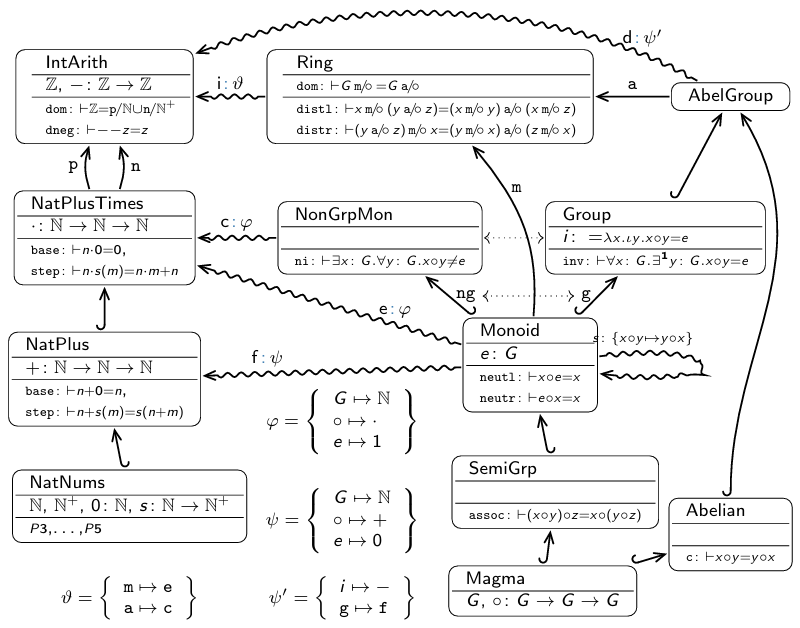
\includegraphics[width=0.7 \linewidth]{images/structures.png}
    \end{center}
\end{figure}
\begin{itemize}
\item nodes are \linkterm{structures}{def:math_structure} with \linkterm{objects}{math_object} ($\circ : \tau$) and properties ($n :\vdash P$).
\item edges represent inheritance
\begin{itemize}
    \item regular inheritance:  $\hookrightarrow$
    \item copying substructures: $\xrightarrow{n}$ 
    \item interpretation via $\varphi$: $\overset{n}{\leadsto}$
\end{itemize} 
\item Examples are just interpretations ($\leadsto$) read backwards
\item Any \linkterm{object}{math_object} / property / \linkterm{theorem}{theorem} can be copied along any edge
\end{itemize}
\labeledsection{Complexity Analysis in AI}{sec:complexity_analysis}
\definition{Algorithm}{
An algorithm is a series of instructions to control a (computation) process.
}{algorithm}

\definition{Computational Problem}{
A computational problem is a triple $\tuple{I, S, \sigma}$, where $I$ is a \linkterm{set}{def:set} of inputs, $S$ is a \linkterm{set}{def:set} of solutions, and $\sigma: I \to \powerset{S}$ asigns to each input the set of valid solutions. The problem is called \textbf{computable} if there exists an algorithm $\alpha : I \to S$ such that for every $i \in I, \alpha (i) \in \sigma (i)$ and $\alpha (i)$ is defined, i.e. the \linkterm{algorithm}{algorithm} always \textbf{halts}.
}{computational_problem}

\definition{Partially Computable Problem}{
A \linkterm{computational problem}{computational_problem} $\tuple{I, S, \sigma}$ is called \textbf{partially computable} if there exists a \textit{partial} \linkterm{algorithm}{algorithm} $\pfunc{\alpha}{I}{S}$ such that for every $i \in I$, if $\alpha (i)$ is defined then $\alpha (i) \in \sigma (i)$. In this case $\alpha$ may diverge on some inputs.
}{partially_computable_problem}

\definition{Resource}{
A resource is a measurable quantity consumed by an \linkterm{algorithm}{algorithm} during execution. The most common resources are
\textbf{time} (number of computation steps) and \textbf{space} (amount of memory used).
}{resource}

\definition{Complexity Theory}{
(Computational) complexity theory focuses on classifying \linkterm{computational problems}{computational_problem} according to their resource usage, and relating these classes to each other.
}{complexity_theory}


\definition{Complexity Measure}{
A complexity measure is a mapping $m : I \to \mathbb{N}$ that assigns to each input $i \in I$ a natural number describing the amount of some \linkterm{resource}{resource} consumed by an \linkterm{algorithm}{algorithm} on input $i$.
}{complexity_measure}

\definition{Input Size}{
The size of an input $i \in I$, denoted $|i|$, is a natural number measuring the length of the encoding of $i$ (for instance, the number of bits required to represent $i$).
}{input_size}

\definition{Asymptotic Analysis}{
Asymptotic analysis studies the growth of a \linkterm{complexity measure}{complexity_measure} as the \linkterm{input size}{input_size} $n$ tends to infinity. It abstracts from constant factors and lower-order terms to capture the long-term behavior of an \linkterm{algorithm}{algorithm}.
}{asymptotic_analysis}


\definition{Running Time}{
If an \linkterm{algorithm}{algorithm} $\alpha$ terminates within $t(n)$ steps on every input of \linkterm{size}{input_size} $n$, then we say that $\alpha$ has \textbf{running time} $T(\alpha) := t$.
}{running_time}

\definition{Time Complexity}{
Let $S \subseteq \mathbb{N} \to \mathbb{N}$ be a \linkterm{set}{def:set} of natural number \linkterm{functions}{function}. An \linkterm{algorithm}{algorithm} $\alpha$ with \linkterm{running time}{running_time} $T(\alpha) = t$ is said to have \textbf{time complexity} in $S$ (written $T(\alpha) \in S$, or colloquially $T(\alpha) = S$) if $t \in S$.
}{time_complexity}

\definition{Space Complexity}{
Let $S \subseteq \mathbb{N} \to \mathbb{N}$ be a \linkterm{set}{def:set} of natural number \linkterm{functions}{function}. An \linkterm{algorithm}{algorithm} $\alpha$ is said to have \textbf{space complexity} in $S$ if, on every input of \linkterm{size}{input_size} $n$, $\alpha$ uses at most $s(n)$ units of memory for some $s \in S$.
}{space_complexity}


\definition{Best-Case Complexity}{
The best-case complexity of an \linkterm{algorithm}{algorithm} $\alpha$ is the function
\[
T^{\text{best}}_\alpha(n) = \min \{ \text{running time of } \alpha(i) \mid i \in I, |i| = n \}.
\]
It describes the minimal resource usage among all inputs of size $n$.
}{best_case_complexity}


\definition{Average-Case Complexity}{
The average-case complexity of an \linkterm{algorithm}{algorithm} $\alpha$ is the expected \linkterm{resource}{resource} usage over all inputs of size $n$, with respect to some probability distribution $D$ on $I$. Formally,
\[
T^{\text{avg}}_\alpha(n) = \mathbb{E}_{i \sim D, |i| = n} [ \text{running time of } \alpha(i) ] .
\]
}{average_case_complexity}

\definition{Worst-Case Complexity}{
The worst-case complexity of an \linkterm{algorithm}{algorithm} $\alpha$ is the function
\[
T^{\text{worst}}_\alpha(n) = \max \{ \text{running time of } \alpha(i) \mid i \in I, |i| = n \}.
\]
It describes the maximal \linkterm{resource}{resource} usage among all inputs of size $n$.
}{worst_case_complexity}

\commandnote{We are mostly interested in \linkterm{worst-case complexity}{worst_case_complexity}.}

\definition{Big-$\mathcal{O}$ Notation}{
In practice, \linkterm{asymptotic analysis}{asymptotic_analysis} is most often applied to the \linkterm{worst-case complexity}{worst_case_complexity}. 
Let $f, g : \mathbb{N} \to \mathbb{R}_{\geq 0}$. 
We say that $f$ is \textbf{asymptotically bounded} by $g$, written $f \in \bigo{g}$ or $f \leq_a g$, if there exist constants $c > 0$ and $n_0 \in \mathbb{N}$ such that
\[
\forall n \geq n_0: \quad f(n) \leq c \cdot g(n).
\]
Equivalently, the \textbf{Landau set} $\mathcal{O}(g)$ is the set of all such \linkterm{functions}{function}:
\[
\mathcal{O}(g) = \{ f \mid \exists c > 0, \exists n_0 \in \mathbb{N}, \forall n \geq n_0 : f(n) \leq c \cdot g(n) \}.
\]
}{big_o}

\textbf{Example: }Let $f(n) = 3n^2 + 2n + 7$ and $g(n) = n^2$.  
We want to show that $f \in \bigo{g}$.  

By the \linkterm{definition of Big-$\mathcal{O}$}{big_o}, this means we must find constants $c > 0$ and $n_0 \in \mathbb{N}$ such that
\[
\forall n \geq n_0 : \quad f(n) \leq c \cdot g(n).
\]

Let's take $n_0 = 1$, then $\forall n \geq 1$ we have:
\[
2n \leq 2n^2 \quad \text{and} \quad 7 \leq 7n^2.
\]

Therefore,
\[
f(n) = 3n^2 + 2n + 7 \;\;\leq\;\; 3n^2 + 2n^2 + 7n^2 = 12n^2.
\]

Here we see that $f(n) \leq 12 \cdot g(n)$ for all $n \geq 1$.  
Thus the definition holds with $c = 12$ and $n_0 = 1$.  
We conclude that $f(n) \in \mathcal{O}(n^2)$.

\Lemma{
\textbf{Growth Ranking}. For $\bar{k}>2$ and $k > 1$ we have:
\[
\bigo{1} \subset \bigo{\operatorname{log}_2 (n)} \subset \bigo{n} \subset \bigo{n^2} \subset \bigo{n^{\bar{k}}} \subset \bigo{k^n} 
\]
}{growth_ranking_complexity}
The following \linkterm{sets}{def:set} are often used for $S$ in $T(\alpha)$:
\begin{table}[h]
\centering
\begin{tabular}{|c|c|c||c|c|c|}
\hline
\textbf{Landau set} & \textbf{class name} & \textbf{rank} &
\textbf{Landau set} & \textbf{class name} & \textbf{rank} \\
\hline
$\mathcal{O}(1)$          & constant     & 1 & $\mathcal{O}(n^2)$ & quadratic   & 4 \\
$\mathcal{O}(\log_2 n)$   & logarithmic  & 2 & $\mathcal{O}(n^k)$ & polynomial  & 5 \\
$\mathcal{O}(n)$          & linear       & 3 & $\mathcal{O}(k^n)$ & exponential & 6 \\
\hline
\end{tabular}
\caption{Common complexity classes}
\end{table}

Computing with \linkterm{Landau sets}{big_o} is quite simple:
\begin{itemize}
    \item $\bigo{ c \cdot f} = \bigo{f}$ for any constant $c \in \mathbb{N}$ (\textit{drop constant factors})
    \item $\bigo{f} \subseteq \bigo{g} \Rightarrow \bigo{f + g} = \bigo{g}$ (\textit{drop low-complexity summands})
    \item $\bigo{f \cdot g} = \bigo{f} \cdot \bigo{g}$ (\textit{distribute over products})
\end{itemize}
\textbf{Example: }$\bigo{4n^3 + 3n + 7^{1000n}} = \bigo{2^n}$ (\textit{exponential})
\commandnote{
   $\bigo{n} \subset \bigo{n \cdot log_2 (n)} \subset \bigo{n^2}$ (\textit{linearithmic})
}

\commandnote{
    \textbf{Updated Growth Ranking \& Common Classes} \\
    To account for all algorithmic patterns discussed (such as nested loops with logarithmic guards ), we refine the growth hierarchy. For $a > 2$ and $b > 1$, the asymptotic ranking is :
    \[
    \bigo{1} \subset \bigo{\log_2 n} \subset \bigo{n} \subset \mathbf{\bigo{n \log_2 n}} \subset \bigo{n^2} \subset \bigo{n^a} \subset \bigo{b^n}
    \]
}

\minititle{Determining the Time/Space Complexity of Algorithms}
Assume we have 
\begin{itemize}
    \item $\Gamma$: a mapping that tells us the complexity of variables.
    \item $\alpha$: a program fragment.
    \item $T_{\Gamma} (\alpha)$: the \linkterm{time complexity}{time_complexity} of $\alpha$ under $\Gamma$.
    \item $C_{\Gamma} (\alpha)$: the context update, i.e. what new cost $\alpha$ introduces.
\end{itemize}
We use \linkterm{induction}{induction} on program strcuture:

\textbf{1. Constant}

If $\alpha = \delta$ (where $\delta$ is a literal, like $5$ or \texttt{true}), then $T_{\Gamma} (\alpha) \in \bigo{1}$

\textbf{2. Variable}

If $\alpha = v$ and $v \in \operatorname{dom}(\Gamma)$, then $T_{\Gamma} (\alpha) \in \bigo{\Gamma (v)}$

\textbf{3. Function Call}

If $\alpha = \varphi (\psi)$, with $T_{\Gamma} (\alpha) \in \bigo{f}$, and $T_{\Gamma \cup C_{\Gamma} (\varphi) \in \bigo{g}}$, then $T_{\Gamma} (\alpha) \in \bigo{\compose{f,g}}$

\textbf{4. Assignment}

If $\alpha = v := \varphi$, with $T_{\Gamma} (\varphi) \in S$, then $T_{\Gamma} (\alpha) \in S$, $C_{\Gamma} (\alpha) = \Gamma \cup (v, S)$

\textbf{5. Composition (sequence)}

If $\alpha = \varphi;\psi$, with $T_{\Gamma} (\varphi) \in P$, and $T_{\Gamma \cup C_{\Gamma}(\varphi)}(\psi) \in Q$, then $T_{\Gamma} (\alpha) \in \operatorname{max}\set{P,Q}$

\textbf{6. Branching}

If $\alpha = $ \texttt{if} $\gamma$ \texttt{then} $\varphi$ \texttt{else} $\psi$ \texttt{end}, with $T_{\Gamma} (\gamma) \in C$, $T_{\Gamma \cup C_{\Gamma}(\gamma)}(\varphi) \in P$, and $T_{\Gamma \cup C_{\Gamma}(\gamma)}(\psi) \in Q$, then $T_{\Gamma} (\alpha) \in \operatorname{max}\set{C,P,Q}$

\textbf{7. Loop}

If $\alpha = $ \texttt{while} $\gamma$ \texttt{do} $\varphi$ \texttt{end}, with $T_{\Gamma}(\gamma) \in \bigo{f}$, and $T_{\Gamma \cup C_{\Gamma}(\gamma)}(\varphi) \in \bigo{g}$, then $T_{\Gamma} (\alpha) \in \bigo{f(n) \cdot g(n)}$

\commandnote{
By default, the overall time complextiy is $T (\alpha) = T_{\phi} (\alpha)$
}

\minititle{Sequence Example}
\begin{verbatim}
x := readArray(n)   -- O(n)
y := sum(x)         -- O(n)
\end{verbatim}
$\operatorname{max}(\bigo{n},\bigo{n}) = \bigo{n}$

\minititle{Conditional Example}
\begin{verbatim}
if isSorted(x) then     -- O(n)
    binarySearch(x,k)   -- O(log n)
else
    linearSearch(x,k)   -- O(n)
end
\end{verbatim}
$\operatorname{max}(\bigo{n}, \bigo{\operatorname{log} (n), \bigo{n}}) = \bigo{n}$

\minititle{While loop example}
\begin{verbatim}
i := 1
while i <= n do 
    i := i + 1
end
\end{verbatim}
Guard (loop condition check) runs $\bigo{n}$ times, body is $\bigo{1}$. Total $\bigo{n \cdot 1} = \bigo{n}$

\minititle{Function Call Example}
Suppose \texttt{buildArray(n)} $\in \bigo{n^2}$ returns an array  of size $n^2$ and \texttt{sort(m)} $\in \bigo{m \cdot \operatorname{log}(m)}$
\begin{verbatim}
sort(buildArray(n))
\end{verbatim}
$\bigo{(n^2) \cdot \operatorname{log} (n^2)} = \bigo{n^2 \cdot \operatorname{log} (n)}$

\minititle{Nested For Loop Example}
\begin{verbatim}
for i = 1 to n do       -- O(n)
    for j = 1 to n do   -- O(n)
        x := x + 1      -- O(1)
\end{verbatim}
Inner loop: $\bigo{n \cdot 1}$, outer loop: $\bigo{n \cdot n \cdot 1}$, total: $\bigo{n^2}$

\minititle{Nested (one logarthmic loop)}
\begin{verbatim}
for i = 1 to n do
    k := 1
    while k < n do
        k := 2 * k
\end{verbatim}
Inner loop starts with $k=1$, each iteration $k$ doubles and the loop stops when $k \geq n$. How many times can we double before reaching $n$? Solve $2^t \geq n \leadsto t = \lceil \operatorname{log}_2 (n) \rceil$. So the inner loop runs $\bigo{\operatorname{log}(n)}$ iterations. Each iteration is $\bigo{1}$, therefore total $\bigo{\operatorname{log}(n)}$.

Outer loop runs exactly $n$ times with each time the cost is $\bigo{\operatorname{log}(n)}$. Total cost is $n \cdot \bigo{\operatorname{log}(n)} = \bigo{n \cdot \operatorname{log}(n)}$

\commandnote{
    Take home message: not every time you see two nested loops you assume $\bigo{n^2}$
}
Here is another example: assume \texttt{<<body>>} $\in \bigo{1}$:
\begin{verbatim}
i, j := 0
while i <= n-1 do
    i := i+1
    while j <= 10 do
        j := j+1
        <<body>>
    end
end
\end{verbatim} 
\textbf{Outer Loop: }$i$ increments by $1$ each time untill $i > n - 1$ we stop, so it runs $n$ times.

\textbf{Inner Loop: }the condition is $j \leq 10$, but note that $j$ is initialized once before the loop and not reset for each $i$! That means, first outer iteration $j=0$, runs until $j = 11$, i.e. $11$ iterations. After that, $j=11$ always and the condition $j \leq 10$ is false, so the inner loop never runs again. Inner loop total cost is $\bigo{11} = \bigo{1}$

Therefore, all in all we have linear time ($\bigo{n}$).


\labeledsection{Formal Languages and Grammars}{sec:formal_langs_grammars}
\definition{Alphabet}{
An alphabet is a \linkterm{finite}{set_cardinality} \linkterm{set}{def:set}; we call each element $a \in A$ a \textbf{character}, and an $n$-tuple $s \in A^n$ a \textbf{string} (of \textit{length} $n$ over $A$).
}{alphabet}

\commandnote{We often write a string $\tuple{c_1, \cdots, c_n}$ as "$c_1 \cdots c_n$", for instance \texttt{"abc"} for $\tuple{a,b,c}$}

\textbf{Example: }Let $A=\set{0,1}$ be an \linkterm{alphabet}{alphabet}
\begin{itemize}
    \item \texttt{"0", "1"} are strings of length $1$ ($A^1 = \set{0,1}$)
    \item \texttt{"00","01","10","11"} are strings of length $2$ in ($A^2$)
    \item \texttt{"001"} $\in A^3$
\end{itemize}



\definition{Empty String}{
Let $A$ be an \linkterm{alphabet}{alphabet}, then $A^0 = \set{\tuple{}}$, where $\tuple{}$ is the unique $0$-tuple. We consider $\tuple{}$ as the string of length $0$ and call it the \textbf{empty string} and denote it with $\epsilon$.
}{empty_string}

\commandnote{
    $\set{1,2,3} = \set{3,2,1}$ BUT $\tuple{1,2,3} \neq \tuple{3,2,1}$ (\linkterm{sets}{def:set} vs strings)
}

\definition{String Length}{
Given a string $s$, we denote its length with $\abs{s}$.
}{string_length}

\definition{String Concatenation}{
The concatenation $\operatorname{conc}(s,t)$ of two strings $s = \tuple{s_1, \cdots, s_n} \in A^n$ and $t = \tuple{t_1,\cdots, t_m} \in A^m$ is defined as $s+t$ or simply \texttt{st}
}{concatenation_string}
\textbf{Example: }$\operatorname{conc}(\text{"text"}, \text{"book"}) = \text{"text"} + \text{"book"} = \text{"textbook"}$.

\definition{Kleene Plus and Kleene Star}{
Let $A$ be an \linkterm{alphabet}{alphabet}, then we define the \linkterm{sets}{def:set}:
\begin{itemize}
    \item $A^{+} := \bigcup_{i \in \mathbb{N}^{+}} A^i$ (\textit{nonempty strings}), and
    \item $A^{*} := A^{+} \cup \set{\epsilon}$ (\textit{strings}).
\end{itemize}
}{kleene_operators}

\definition{Formal Language}{
A \linkterm{set}{def:set} $L \subseteq A^{*}$ is called a \textit{formal language} over $A$.
}{formal_language}

\textbf{Example: }If $A = \set{a,b}$ then:
\[
A^{*} = \bigcup_{n = 0}^{\infty} A^n
\]
where $A^0 = \epsilon$, $A^1 = \set{a,b}$, $A^2 = \set{a, b, ab, ba}$, and so on ... 
\begin{align*}
    A^{*} &= \set{\epsilon, a, b, aa, ab, ba, bb, aaa, aab, aba, abb, \cdots} \\
    A^{+} &= \set{a, b, aa, ab, ba, bb, aaa, aab, aba, abb, \cdots} \\
\end{align*}
A \linkterm{formal language}{formal_language} might be $L = \set{a,b,aab,bbb, \cdots}$

\definition{Repeating Chars}{
We use $c^{[n]}$ for the string that consists of the character \texttt{c} repeated $n$ times.
}{repeating_chars}
\textbf{Examples: }
\begin{itemize}
    \item Let $A = \set{a,b}$, $a^{[5]} = $ \texttt{"aaaaa"}.
    \item The \linkterm{set}{def:set} $M := \set{\text{ba}^{[n]} \mid n \in \mathbb{N}}$ of strings that start with character $b$ followd by an arbitrary numbers of a's is a \linkterm{formal language}{formal_language} over $A = \set{a,b}$
\end{itemize}

\commandnote{A \linkterm{formal language}{formal_language} might be infinite and even undecidable even if the \linkterm{alphabet}{alphabet} $A$ is \linkterm{finite}{set_cardinality}. For example, let $A = \set{a,b}$ then the \linkterm{formal language}{formal_language} $L = \set{a,ab,bba}$ is \linkterm{finite}{set_cardinality} but the \linkterm{formal language}{formal_language} $L = \setbuilder{a^{[n]}}{n \in \mathbb{N}}$ is infinite.}

Since we cannot list all strings in a \linkterm{formal language}{formal_language} $L$ because there are infinitely many, we need a \textbf{finite description} that can generate all strings in $L$. We need \textbf{Grammars}.

\definition{Phrase Structure Grammar}{
A phrase structure grammar (\textit{type 0 grammar, unrestricted grammar, grammar}) is a tuple $\tuple{N,\Sigma, P, S}$ where
\begin{itemize}
    \item $N$ is a \linkterm{finite}{set_cardinality} \linkterm{set}{def:set} of \textbf{nonterminal symbols},
    \item $\Sigma$ is a \linkterm{finite}{set_cardinality} \linkterm{set}{def:set} of \textbf{terminal symbols}. (members of $N \cup \Sigma$ are called symbols).
    \item $P$ is a \linkterm{finite}{set_cardinality} \linkterm{set}{def:set} of \textbf{production rules}: pairs $p := h \to b$ (also written as $h \Rightarrow b$), where $h \in (\Sigma \cup N)^{*} N (\Sigma \cup N)^{*}$ and $b \in (\Sigma \cup N)^{*}$. The string $h$ is called the \textbf{head} of $p$ and $b$ the \textbf{body}.
    \item $S \in N$ is a distinguished symbol called the \textbf{start symbol} (also \textbf{sentence symbol}).
\end{itemize}
The \linkterm{sets}{def:set} $N$ and $\Sigma$ are assumed to be \linkterm{disjoint}{disjoint}. Any word $w \in \Sigma^{*}$ is called a \textbf{terminal word}.
}{phrase_structure_grammar}
\commandnote{\linkterm{Production rules}{phrase_structure_grammar} map strings with at least one \linkterm{nonterminal}{phrase_structure_grammar} to arbitrary other strings}

\textbf{Notation: }If we have $n$ \linkterm{production rule}{phrase_structure_grammar} $h \to b_i$ sharing a head, we often write $h \to b_1 \mid \cdots \mid b_n$ instead.

\textbf{Example: }A simple \linkterm{grammar}{phrase_structure_grammar} for english sentences:
\begin{align*}
\text{S} &::= \text{NP} \text{ Vi} \\
\text{NP} &::= \text{Article} \text{ N} \\
\text{Article} &::= \text{the} \mid \text{a} \mid \text{an} \\
\text{N} &::= \text{dog} \mid \text{teacher} \mid \cdots \\
\text{Vi} &::= \text{sleeps} \mid \text{smells} \mid \cdots
\end{align*}
Here $S$ is the \linkterm{start symbol}{phrase_structure_grammar}, NP, Article, N, and Vi are \linkterm{nonterminals}{phrase_structure_grammar}, the, a, dog, smells, ... are \linkterm{terminals}{phrase_structure_grammar}. Let's generate a valid sentence from the \linkterm{grammar}{phrase_structure_grammar}:
\begin{verbatim}
NP           Vi
Article N    Vi
the     N    Vi
the    dog   Vi
the    dog sleeps
\end{verbatim}

\definition{Lexical}{
A \linkterm{production rule}{phrase_structure_grammar} whose head is a single \linkterm{nonterminal}{phrase_structure_grammar} and whose body consists of a single \linkterm{terminal}{phrase_structure_grammar} is called \textbf{lexical} or a \textbf{lexical insertion rule}.
}{lexical_rule_grammar}
\textbf{Example: } Both of the following \linkterm{rules}{phrase_structure_grammar} are \linkterm{lexical}{lexical_rule_grammar}
\begin{align*}
\text{Noun } &\to \text{ "dog"} \\
\text{Verb } &\to \text{ "run"} 
\end{align*}

\definition{Lexicon of a Grammar}{
The \linkterm{subset}{subset} of \linkterm{lexical rules}{lexical_rule_grammar} of a \linkterm{grammar}{phrase_structure_grammar} $G$ is called the \textbf{lexicon} of $G$
}{lexicon_grammar}

\definition{Vocabulary}{
The \linkterm{set}{def:set} of body symbols are called the vocabulary (or the alphabet).
}{vocabulary_grammar}

\definition{Lexical Categories of a Grammar}{
The \linkterm{nonterminals}{phrase_structure_grammar} that appear in the heads of \linkterm{lexical}{lexical_rule_grammar} rules are called lexical categories of the \linkterm{grammar}{phrase_structure_grammar}.
}{lexical_categories_grammar}

\definition{Structural Rules}{
The non \linkterm{lexicon}{lexicon_grammar} \linkterm{production rules}{phrase_structure_grammar} are called structural.
}{structural_rules_grammar}

\definition{Phrasal categories}{
The \linkterm{nonterminals}{phrase_structure_grammar} in the heads of \linkterm{production rules}{phrase_structure_grammar} that expand into other \linkterm{nonterminals}{phrase_structure_grammar} are called phrasal (syntactic) categories.
}{phrasal_categories}

\definition{$G$-Derivation}{
Given a \linkterm{phrase structure grammar}{phrase_structure_grammar} $G := \set{N,\Sigma, P, S}$, we say $G$ \textbf{derives} $t \in (\Sigma \cup N)^{*}$ from $s \in (\Sigma \cup N)^{*}$ in one step, iff there is a \linkterm{production rule}{phrase_structure_grammar} $p \in P$ with $p = h \to b$ and there are $u,v \in (\Sigma \cup N)^{*}$, such that $s=uhv$ and $t=ubv$. We write $s \to_{G}^{p} t$ (or $s \to_{G} t$ if $p$ is clear from the context) and use $\to_{G}^{*}$ for the \linkterm{reflexive}{reflexive} \linkterm{transitive}{transitive_relation} closure of $\to_G$. We call $s \to_{G}^{*} t$ a $G$-derivation of $t$ from $s$.
}{g_derivation_grammar}

Let's unravel that. Take the following \linkterm{grammar}{phrase_structure_grammar}:
\begin{itemize}
    \item $N = \set{S}$
    \item $\Sigma = \set{a,b}$
    \item $P = \set{S \to \text{aSb}, S \to \text{ab}}$
    \item $S = S$
\end{itemize}
The following derivations holds:
\begin{itemize}
    \item $S \to_{G}^{p} \text{aSb}$ where $p: S \to \text{aSb}$ (\textit{one step})
    \item $\text{aSb} \to_{G}^{q} \text{aabb}$ where $q: S \to \text{ab}$ (\textit{one step})
    \item $S \to_{G}^{S \to \text{aSb}} \text{aSb} \to_{G}^{S \to \text{ab}} \text{aabb}$ (\textit{multiple steps}). So, $S \to_{G}^{*} \text{aabb}$
\end{itemize}


\definition{Sentential Form}{
Given a \linkterm{phrase structure grammar}{phrase_structure_grammar} $G := \set{N,\Sigma, P, S}$, we say that $s \in (\Sigma \cup N)^{*}$ is a \textbf{sentential form} of $G$, iff $S \to_{G}^{*} s$
}{sentential_form}

\definition{Sentence}{
A \linkterm{sentential form}{sentential_form} that does not contain \linkterm{nonterminals}{phrase_structure_grammar} is called a sentence of $G$, we also say that $G$ \textbf{accepts} $s$. We say that $G$ \textbf{rejects} $s$, iff it is not a sentence of $G$.
}{sentence_grammar}

\textbf{Examples}

1. "Article teacher Vi" is a \linkterm{sentential form}{sentential_form}
\begin{align*}
S &{\to_G} \text{ NP } \text{ Vi } \\
&{\to_G} \text{ Article } \text{ N } \text{ Vi } \\
&{\to_G} \text{ Article } \text{ teacher } \text{ Vi }
\end{align*}

2. "the teacher sleeps" is a \linkterm{sentence}{sentence_grammar}
\begin{align*}
S &{\to_G^{*}} \text{ Article } \text{ teacher } \text{ Vi } \\
&{\to_G} \text{ the } \text{ teacher } \text{ Vi } \\
&{\to_G} \text{ the } \text{ teacher } \text{ sleeps }
\end{align*}


\definition{Language Generation}{
The language $L(G)$ of $G$ is the \linkterm{set}{def:set} of its \linkterm{sentences}{sentence_grammar}. We say that $L(G)$ is \textbf{generated} by $G$.
}{language_generation_grammar}

\definition{Equivalent Grammars}{
We call two \linkterm{grammars}{phrase_structure_grammar} \textbf{equivalent}, iff they have the same \linkterm{languages}{language_generation_grammar}.
}{equivalent_grammars}

\definition{Universal Grammar}{
A \linkterm{grammar}{phrase_structure_grammar} $G$ is said to be \textbf{universal} if $L(G) = \Sigma^{*}$
}{universal_grammar}

\definition{Syntactic Analysis}{
Syntactic analysis (parsing / syntax analysis) is the process of analyzing a string of symbols, either in a \linkterm{formal}{formal_language} or a \linkterm{natural language}{natural_language} by means of a \linkterm{grammar}{phrase_structure_grammar}.
}{syntactic_analysis_grammar}

\commandnote{The shape of the \linkterm{grammar}{phrase_structure_grammar} determines the size of its \linkterm{language}{language_generation_grammar}}

\definition{Context-Sensitive}{
We call a \linkterm{grammar}{phrase_structure_grammar} context-sensitive (or type 1), if the bodies of \linkterm{production rules}{phrase_structure_grammar} have no less symbols than the heads.
}{contex_sensitive_grammar}
\textbf{Example:} The \linkterm{language}{formal_language} $\set{a^{[n]}  b^{[n]}  c^{[n]}}$ is \linkterm{accepted}{sentence_grammar} by
\begin{align*}
S \quad &{\to} \quad \text{a b c} \mid A \\
A \quad &{\to} \quad \text{a } A \text{ } B \text{ c} \mid \text{a b c} \\
\text{c } B \quad &{\to} \quad B \text{ c} \\
\text{b } B \quad &{\to} \quad \text{b b}
\end{align*}


\definition{Context-Free}{
We call a \linkterm{grammar}{phrase_structure_grammar} context-free (or type 2), iff the heads have exactly one symbol.
}{contex_free_grammar}

\textbf{Example: }The \linkterm{language}{formal_language} $\set{a^{[n]}  b^{[n]}}$ is  \linkterm{accepted}{sentence_grammar} by $S \to \text{ a } S \text{ b } \mid \text{ } \epsilon$

\definition{Regular}{
We call a \linkterm{grammar}{phrase_structure_grammar} regular (or type 3, or REG), if additionally the bodies are empty or consist of a \linkterm{nonterminal}{phrase_structure_grammar}, optionally followed by a \linkterm{terminal symbol}{phrase_structure_grammar}.
}{regular_grammar}

\textbf{Example: }The \linkterm{language}{formal_language} $\set{a^{[n]}}$ is \linkterm{accepted}{sentence_grammar} by $S \to S \text{ a } \mid \text{ } \epsilon$


\commandnote{
By extension, a \linkterm{formal language}{formal_language} $L$ is called \textit{context-sensitive / context-free / regular}, iff it is the \linkterm{language}{language_generation_grammar} of a respective \linkterm{grammar}{phrase_structure_grammar}. \linkterm{Context-free grammars}{contex_free_grammar} are sometimes \texttt{CFGs} and context-free languages \texttt{CFLs}.
}

\textbf{Observation: }\linkterm{Natural languages}{natural_language} are probably \linkterm{context sensitive}{contex_sensitive_grammar} but parsable in real time!
\labeledsection{Term Languages and Abstract Grammars}{sec:term_langs_abstract_grams}
\commandnote{
In most applications of \linkterm{symbolic AI}{symbolicai}, the \linkterm{formal languages}{formal_language} are very strucutred.
}

\textbf{Example (\linkterm{Arithmetic}{arithmetic} Expressions): }Consider the \linkterm{CFG}{contex_free_grammar} $G$ and the $G$-derivation:

\begin{verbatim}
term   → num | var | sum | prod | neg
num    → digit*
digit  → 1 | 2 | 3 | 4 | 5 | 6 | 7 | 8 | 9 | 0
var    → 'x' num
sum    → '(' term '+' term ')'
prod   → '(' term '*' term ')'
neg    → '-(' term ')'

term → G -(term)
     → G -((term * term))
     → G -(((term + term) * num))
     → G -(((var + num) * digit digit))
     → G -(((x num + digit*) * 555))
     → G -(((x digit digit + 3) * 555))
     → G -(((x29 + 3) * 555))
\end{verbatim}
$G$ accepts the string $-(((X29+3) * 555))$ but not $-(X29*3($.

\commandnote{
We call such \linkterm{languages}{formal_language} term languages
}

\textbf{Observation: }Strings in $L(G)$ are \textit{well-bracketed} and can be split into sub-strings from $L(G)$.

\textbf{Intuition: }The parse \linkterm{trees}{tree} are the primary \linkterm{objects}{math_object} for \linkterm{symbolic AI}{symbolicai}, the strings are just the technical I/O.

\definition{Parse Tree}{
Let $G$ be a \linkterm{CFG}{contex_free_grammar} that accepts a string $s$. Then a \textbf{parse tree} is a \linkterm{node labeled}{labeled_graph}, ordered \linkterm{tree}{tree} $P_s$ that represents the syntactic strucutre of $s$.
}{parse_tree}
\textbf{Example: }the \linkterm{parse tree}{parse_tree} of "the teacher sleeps":
\begin{verbatim}
        S
       / \
     NP   Vi
    /  \    \
Article N   sleeps
   |    |
  the teacher  
\end{verbatim}

\commandnote{
There may be multiple derivations that accept a string $s$ in a \linkterm{CFG}{contex_free_grammar}. For example, $S \to \text{ NP } \text{Vi} \to \text{ Article N } \text{Vi} \cdots$ or $S \to \text{ NP } \text{Vi} \to \text{ NP } \text{sleeps} \cdots$, and so on.
}

Let $G$ be \linkterm{CFG}{contex_free_grammar} and $D := s \to_{G}^{*} t$ a $G$-derivation where $t$ is a \linkterm{sentence}{sentence_grammar} of $G$. We define the \linkterm{parse tree}{parse_tree} $P_D$ of $D$ \linkterm{recursively}{recursion}:
\begin{itemize}
\item IF $D = s \to_{G}^{p} t$, then $p$ is a \linkterm{lexical}{lexical_grammar} \linkterm{rule}{phrase_structure_grammar} $s\to t$ and $t$ consists of a single \linkterm{terminal}{phrase_structure_grammar}. Then $P_D$ is the \linkterm{tree}{tree} whose root has label $s$ with one child labeled with $t$.
\item If $D = s \to_{G}^{p} \bar{s} \to_{G}^{*} t$, $\bar{s} \to_{G}^{*} t$, and $p = h \to a_1 \cdots a_n$, then the root of $P_D$ has label $h$ and it has children that are the \linkterm{parse trees}{parse_tree} for the subderivations for the $a_i$ in $\bar{D}$.
\end{itemize}

\commandnote{Term languages are ones that have enough structural characters so that the \linkterm{parse tree}{parse_tree} is obvious.}

In \linkterm{SML}{def:sml} we can program the same \linkterm{grammar}{phrase_structure_grammar} as an abstract datatype:
\begin{verbatim}
datatype aterm =
    anum of int
  | avar of int
  | aneg of aterm
  | asum of aterm * aterm
  | aprod of aterm * aterm;
\end{verbatim}

And we can express arithmetic expressions as \linkterm{SML}{def:sml} expressions directly, e.g. $-(((X29+3) * 555))$:
\begin{verbatim}
- val ex = aneg (aprod (asum (avar 29, anum 3), anum 555));
val ex = aneg (aprod (asum (avar 29,anum 3),anum 555)) : aterm
\end{verbatim}

Moreover, we can traverse the term \linkterm{recursively}{recursion} and print it as a string:
\begin{verbatim}
fun aprint (anum n) = Int.toString n
  | aprint (avar n) = "x" ^ Int.toString n
  | aprint (aneg t) = "-(" ^ aprint t ^ ")"
  | aprint (asum (t1, t2)) = "(" ^ aprint t1 ^ "+" ^ aprint t2 ^ ")"
  | aprint (aprod (t1, t2)) = "(" ^ aprint t1 ^ "*" ^ aprint t2 ^ ")";
\end{verbatim}

Let's test that on our \texttt{ex}:
\begin{verbatim}
- aprint ex;
val it = "-(((x29+3)*555))" : string
\end{verbatim}

We can also do more complex tasks via \linkterm{tree}{tree} traversal. For example, we can evaluate \texttt{"-(((x29+3)*555))"}. To do that, we need to know the value of the variable $X29$. This is traditionally given by an assignment that assigns values to variables, e.g. $X1 \mapsto 3, X29 \mapsto 5, \cdots$ (a dictionary), which we can represent as a list of pairs in \linkterm{SML}{def:sml}:
\begin{verbatim}
type assignment = (int * aterm) list
\end{verbatim}
Then we can represent the evaluation function by \linkterm{recursion}{recursion} over the structure of the expression:
\begin{verbatim}
fun aeval (anum n, a:assignment) = n
|   aeval (aneg (n), a) = ~(aeval (n,a))
|   aeval (asum (s,t), a) = aeval (s,a) + aeval (t,a)
|   aeval (aprod (s,t), a) = aeval (s,a) * aeval (t,a);
\end{verbatim}
In all cases, the assignment is just passed on to the \linkterm{recursive call}{recursion}. The only exception is the variable case, where we need to \linkterm{recursively}{recursion} find the right value from the assignment, so the final function would look like:
\begin{verbatim}
fun aeval (anum n, a) = n
  | aeval (aneg t, a) = ~ (aeval (t, a))
  | aeval (asum (s, t), a) = aeval (s, a) + aeval (t, a)
  | aeval (aprod (s, t), a) = aeval (s, a) * aeval (t, a)
  | aeval (avar n, []) = raise Fail "unbound variable"
  | aeval (avar n, (m, r) :: l) =
      if n = m then aeval (r, l) else aeval (avar n, l);
\end{verbatim}

Let's first assign $X29 \mapsto 5$
\begin{verbatim}
val env = [(29, anum 5)];
\end{verbatim}
Then test the function on our term:
\begin{verbatim}
- val ex = aneg (aprod (asum (avar 29, anum 3), anum 555));
val ex = aneg (aprod (asum (avar 29,anum 3),anum 555)) : aterm

- val result = aeval (ex, env);
val result = ~4440 : int
\end{verbatim}

\commandnote{
The situation for \linkterm{arithmetic}{arithmetic} expressions in \linkterm{SML}{def:sml} is typical for term languages.
\begin{itemize}
    \item Inductive data types, one constructor per \linkterm{production rule}{phrase_structure_grammar}
    \item Expressions as \linkterm{tree}{tree}-structured data structures (no brackets needed)
    \item All computation on expressions via \linkterm{recursive}{recursion} \linkterm{tree}{tree} traversal
\end{itemize}
}

\definition{Tree Grammar}{
A tree grammar is a \linkterm{grammar}{phrase_structure_grammar} where the result data type is \linkterm{trees}{tree} not strings.
}{tree_grammar}
If we interpret the brackets as "\linkterm{parse tree}{parse_tree} constructors", then we do not have to worry about matching them. The string representation - with e.g. infix notations for operators - is just a derived / secondary artifact for storage / communication (implementation details).

\definition{Abstract vs Concrete Grammars}{
The underlying \linkterm{tree}{tree} \linkterm{grammar}{phrase_structure_grammar} of a \linkterm{language}{formal_language} is often called the \textbf{abstract grammar}; it captures the essence of the \linkterm{formal language}{formal_language} (the constructors), and any derived (string) \linkterm{grammar}{phrase_structure_grammar} - there may be multiple - is called a \textbf{concrete grammar}; they correspond to, e.g. the results of print functions.
}{abstract_concrete_grammar}

\commandnote{We are mostly interested in \linkterm{\textbf{abstract grammars}}{abstract_concrete_grammar} in \linkterm{symbolic AI}{symbolicai}}


\include{search}
\include{csp}
\include{formal_systems}
\include{pl0}
\include{atp_pl0}
\include{pl1}
\include{atp_pl1}
\labeledsection{Logic-Based Knowledge Representation}{sec:kr}
\definition{Semantic Network}{
A semantic network is a \linkterm{directed graph}{directed_graph} for representing knowledge:
\begin{itemize}
    \item \linkterm{nodes}{tree} represent \textbf{objects} and \textbf{concepts} (classes of objects)
    \item \linkterm{edges}{directed_graph} (called links) represent relations between these
\end{itemize}
}{semantic_network}

\definition{Inclusion}{
We call links labeled by \textit{isa} inclusion links or isa links (inclusion of concepts)
}{isa}

\definition{Instance}{
We call links labeled by \textit{inst} instance links or inst links (concept memership)
}{inst}

\definition{Relations in Semantic Nets}{
We call all links labels \textbf{except} \linkterm{isa}{isa} and \linkterm{inst}{inst} in a \linkterm{semantic network}{semantic_network} \textbf{relations}.
}{relations_sn}

\definition{Inference in Semantic Networks}{
Let $N$ be a \linkterm{semantic network}{semantic_network} and $R$ a \linkterm{relation}{relations_sn} in $N$ such that $A \xrightarrow{\linkterm{isa}{isa}} B \xrightarrow{R} C$ or $A \xrightarrow{\linkterm{inst}{inst}} B \xrightarrow{R} C$, then we can derive a \linkterm{relation}{relations_sn} $A \xrightarrow{R} C$ in $N$. The process of deriving new concepts and \linkterm{relation}{relations_sn} from existing ones is called \textbf{inference} and concepts/\linkterm{relation}{relations_sn} that are only available via inference are called \textbf{implicit} in a \linkterm{semantic network}{semantic_network}.
}{inference_sn}

\textbf{Example: } blue are \linkterm{derived}{inference_sn} \linkterm{relations}{relations_sn}, red is not allowed:
\begin{figure}[H]
    \centering
    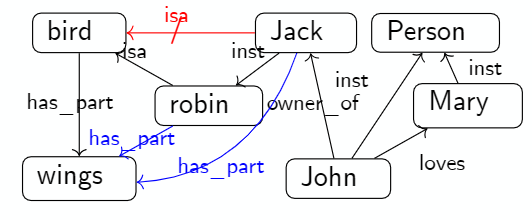
\includegraphics[width=0.4\linewidth]{images/derived_relations_sn.png}
    \caption{\linkterm{Inference}{inference_sn} in \linkterm{semantic networks}{semantic_network}}
    \label{fig:derived_relations}
\end{figure}

\definition{TBox}{
We call the subgraph of a \linkterm{semantic network}{semantic_network} $N$ spanned by the \linkterm{isa links}{isa} and \linkterm{relations}{relations_sn} between \textbf{concepts} the \textbf{terminology} (or \textbf{TBox}, or \textbf{Isa Hierarchy}).
}{tbox}

\definition{ABox}{
We call the subgraph of a \linkterm{semantic network}{semantic_network} $N$ spanned by the \linkterm{inst links}{inst} and \linkterm{relations}{relations_sn} between \textbf{objects} the \textbf{assertions} (or \textbf{ABox}).
}{abox}

\textbf{Example: }
\begin{figure}[H]
    \centering
    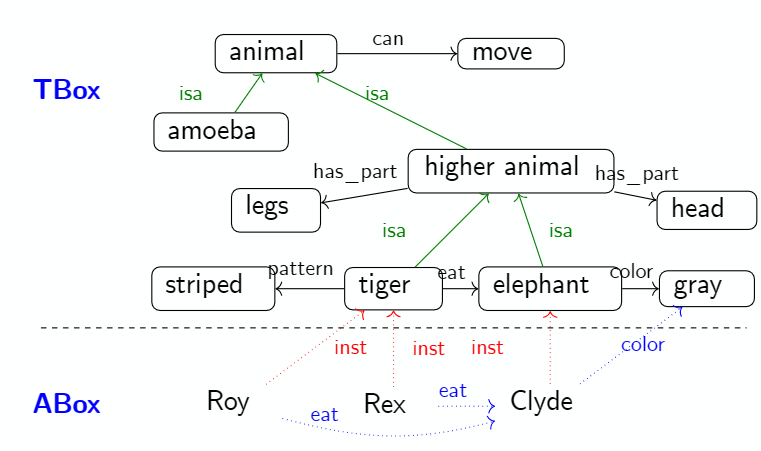
\includegraphics[width=0.4\linewidth]{images/abox_tbox.png}
    \caption{\linkterm{TBox}{tbox} and \linkterm{ABox}{abox} in \linkterm{semantic networks}{semantic_network}}
    \label{fig:tbox_abox}
\end{figure}

\definition{$\text{PL}^0_{\text{DL}}$}{
We use \linkterm{propositional logic}{def:pl0_as_ls} as a \linkterm{set}{def:set} description language. We define $\text{PL}^0_{\text{DL}}$ by the following \linkterm{grammar}{phrase_structure_grammar} for the $\text{PL}^0_{\text{DL}}$ concepts (formulae):
\[
\mathcal{L} ::= C \mid \top \mid \bot \mid \overline{\mathcal{L}} \mid \mathcal{L} \sqcap \mathcal{L} \mid \mathcal{L} \sqcup \mathcal{L} \mid \mathcal{L} \sqsubseteq \mathcal{L} \mid \mathcal{L} \equiv \mathcal{L}
\]
}{pl0dl}

\linkterm{$\text{PL}^0_{\text{DL}}$}{pl0dl} is formed from:
\begin{itemize}
    \item \linkterm{atomic formulae}{atomic_formula}
    \item concept intersection ($\sqcap$)
    \item concept complement ($\overline{\cdot}$)
    \item concept union ($\sqcup$)
    \item concept subsumption ($\sqsubseteq$), and equivalence ($\equiv$)
\end{itemize}

\definition{Set-Theoretic Semantics of \linkterm{$\text{PL}^0_{\text{DL}}$}{pl0dl}}{
Let $\mathcal{D}$ be a given \linkterm{set}{def:set} (\linkterm{domain of discourse}{domain_of_discourse}) and $\func{\varphi}{\mathcal{V}_{\text{PL}^0}}{\powerset{\mathcal{D}}}$. We define the valuation $\sint{\cdot}$ as:
\begin{itemize}
    \item $\sint{P} := \varphi(P)$ (for atomic concepts)
    \item $\sint{\top} := \mathcal{D}$ and $\sint{\bot} := \emptyset$
    \item $\sint{\overline{A}} := \mathcal{D} \setminus \sint{A}$ 
    \item $\sint{A \sqcap B} := \sint{A} \cap \sint{B}$ 
    \item $\sint{A \sqcup B} := \sint{A} \cup \sint{B}$ 
    \item $\sint{A \sqsubseteq B}$ is satisfied iff $\sint{\overline{A}} \cup \sint{B} = \mathcal{D}$ which is satisfied iff $\sint{A} \subseteq \sint{B}$ 
    \item $\sint{A \equiv B}$ is satisfied iff $\sint{A} = \sint{B}$ 
\end{itemize}
}{set_theoretic_semantics_pl0dl}

\commandnote{
The triple $\langle \text{PL}^0_{\text{DL}}, \mathcal{S}, \sint{\cdot} \rangle$, where $\mathcal{S}$ is the class of possible domains, forms a \linkterm{logical system}{logical_system}.
}

\definition{Concept Axiom}{
A concept axiom is a \linkterm{$\text{PL}^0_{\text{DL}}$}{pl0dl} formula $A$ that is assumed to be true in the world.
}{concept_axiom}

\definition{Set-Theoretic Semantics of Axioms}{
$A$ is true in \linkterm{domain of discourse}{domain_of_discourse} $\mathcal{D}$ iff $\sint{A} = \mathcal{D}$
}{set_theoretic_semantics_axioms}

\commandnote{
Any concept we add to our world is just a \linkterm{set}{def:set}, for example, here is a world with three concepts (no \linkterm{concept axioms}{concept_axiom} yet):

\begin{figure}[H]
    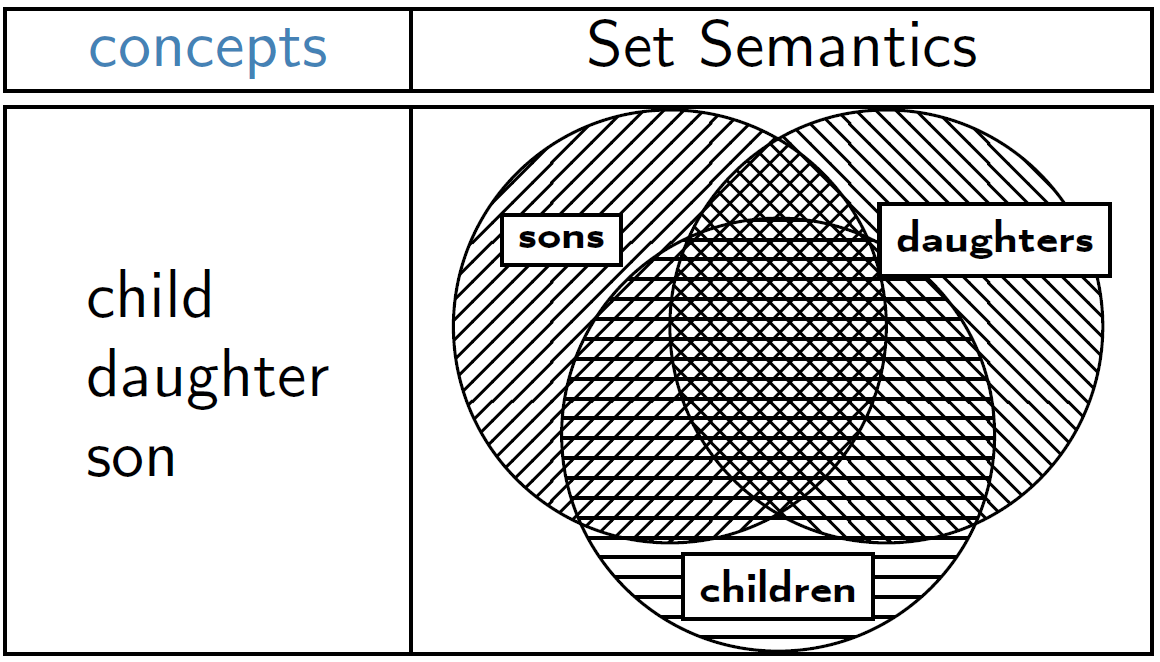
\includegraphics[width=0.4\linewidth]{images/concepts_sets1.png}
\end{figure}

Looks a mess? try to add \linkterm{concept axioms}{concept_axiom}. Here is how it looks like when adding:
\begin{itemize}
    \item $\text{son} \sqsubseteq \text{child}$
    \item $\text{daughter} \sqsubseteq \text{child}$
\end{itemize}

\begin{figure}[H]
    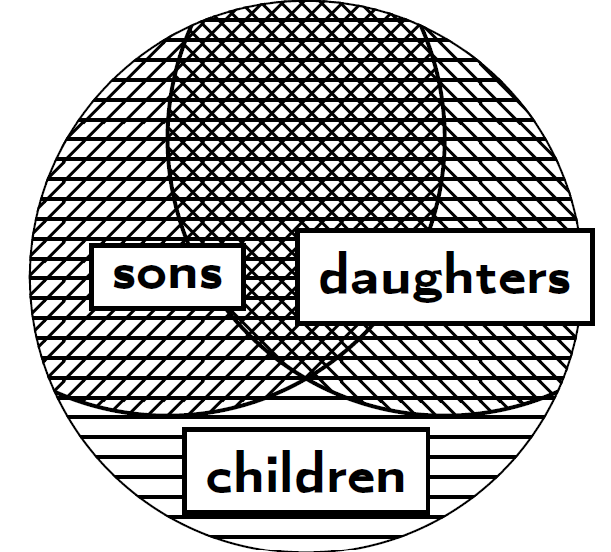
\includegraphics[width=0.2\linewidth]{images/concepts_sets2.png}
\end{figure}

We add two more \linkterm{concept axioms}{concept_axiom}:
\begin{itemize}
    \item $\overline{\text{son} \sqcap \text{daughter}}$
    \item $\text{child} \sqsubseteq \text{son} \sqcup \text{daughter}$
\end{itemize}

\begin{figure}[H]
    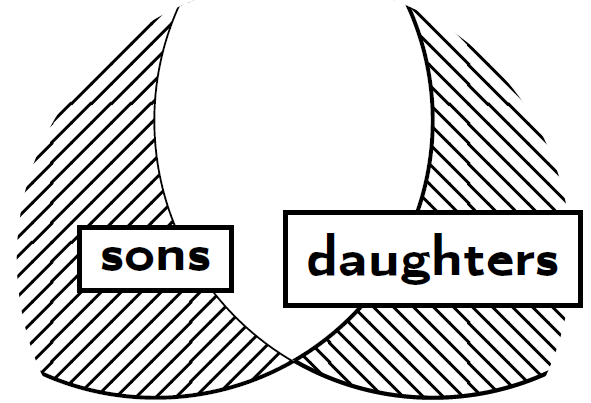
\includegraphics[width=0.2\linewidth]{images/concepts_sets3.png}
\end{figure}

}

The set-theoretic semantics is compatible with the regular semantics of \linkterm{propositional logic}{def:pl0_as_ls}, therefore we have the same \linkterm{propositional identities}{identities_pl0}:

\begin{table}[h]
\centering
\caption{\linkterm{$\text{PL}^0_{\text{DL}}$}{pl0dl} Identities}
\label{tab:identities_pl0dl}
\begin{tabular}{|l|c|c|}
\hline
\textbf{Name} & \textbf{for $\sqcap$} & \textbf{for $\sqcup$} \\
\hline
Idempotence      & $\varphi \sqcap \varphi = \varphi$        & $\varphi \sqcup \varphi = \varphi$ \\
Identity         & $\varphi \sqcap \top = \varphi$            & $\varphi \sqcup \bot = \varphi$ \\
Absorption 1     & $\varphi \sqcap \bot = \bot$                & $\varphi \sqcup \top = \top$ \\
Commutativity    & $\varphi \sqcap \psi = \psi \sqcap \varphi$ & $\varphi \sqcup \psi = \psi \sqcup \varphi$ \\
Associativity    & $\varphi \sqcap (\psi \sqcap \theta) = (\varphi \sqcap \psi)\sqcap \theta$  
                 & $\varphi \sqcup (\psi \sqcup \theta) = (\varphi \sqcup \psi)\sqcup \theta$ \\
Distributivity   & $\varphi \sqcap (\psi \sqcup \theta)= (\varphi \sqcap \psi)\sqcup (\varphi \sqcap \theta)$ 
                 & $\varphi \sqcup (\psi \sqcap \theta)= (\varphi \sqcup \psi)\sqcap (\varphi \sqcup \theta)$ \\
Absorption 2     & $\varphi \sqcap (\varphi \sqcup \theta)= \varphi$ 
                 & $\varphi \sqcup (\varphi \sqcap \theta)= \varphi$ \\
De Morgan rule   & $\overline{\varphi \sqcap \psi}= \overline{\varphi} \sqcup \overline{\psi}$ 
                 & $\overline{\varphi \sqcup \psi} = \overline{\varphi} \sqcap \overline{\psi}$ \\
double negation  & \multicolumn{2}{c|}{$\overline{\overline{\varphi}}  = \varphi$} \\
\hline
\end{tabular}
\end{table}


\definition{Translation to \linkterm{$\text{PL}^1$}{pl1}}{
We define the translation of \linkterm{$\text{PL}^0_{\text{DL}}$}{pl0dl} expressions into \linkterm{$\text{PL}^1$}{pl1} using two functions: a recursive mapping $\text{FOL}_x$ for concept expressions and a top-level mapping $\text{FOL}$ for axioms/formulae.
}{mapping_pl0dl_pl1}

\textbf{Recursive mapping for Concepts:}

\begin{tabular}{@{}l@{}}
    $\text{FOL}_x(p) := p(X)$ \\
    $\text{FOL}_x(\overline{A}) := \neg \text{FOL}_x(A)$ \\
    $\text{FOL}_x(A \sqcap B) := \text{FOL}_x(A) \land \text{FOL}_x(B)$ \\
    $\text{FOL}_x(A \sqcup B) := \text{FOL}_x(A) \lor \text{FOL}_x(B)$ \\
    $\text{FOL}_x(A \sqsubseteq B) := \text{FOL}_x(A) \Rightarrow \text{FOL}_x(B)$ \\
    $\text{FOL}_x(A \equiv B) := \text{FOL}_x(A) \Leftrightarrow \text{FOL}_x(B)$ \\
\end{tabular}

\textbf{Mapping for Formulae (calls $\text{FOL}_x$):}
\begin{tabular}{@{}l@{}}
    $\text{FOL}(A) := \forall X. \, \text{FOL}_x(A)$ \\
\end{tabular}

\textbf{Example: }
Let's translate the formula: \textit{"an undergrad is a person who is not a graduate"}. In \linkterm{$\text{PL}^0_{\text{DL}}$}{pl0dl}, we can express this by:
\[
\text{undergrad} \equiv \text{person} \sqcap \overline{\text{graduate}}
\]

\begin{align*}
\text{FOL}(\text{undergrad} \equiv \text{person} \sqcap \overline{\text{graduate}}) &= \forall X. \text{FOL}_x(\text{undergrad} \equiv \text{person} \sqcap \overline{\text{graduate}}) \\
\text{FOL}_x(\text{undergrad} \equiv \text{person} \sqcap \overline{\text{graduate}}) &= \text{FOL}_x(\text{undergrad}) \Leftrightarrow \text{FOL}_x(\text{person} \sqcap \overline{\text{graduate}}) \\
\text{FOL}_x(\text{undergrad}) &= \text{undergrad}(X) \\
\text{FOL}_x(\text{person} \sqcap \overline{\text{graduate}}) &= \text{FOL}_x(\text{person}) \land \text{FOL}_x(\overline{\text{graduate}}) \\
&= \text{person}(X) \land \neg \text{FOL}_x(\text{graduate}) \\
&= \text{person}(X) \land \neg \text{graduate}(X) \\
\text{FOL}(\text{undergrad} \equiv \text{person} \sqcap \overline{\text{graduate}}) &= \forall X. (\text{undergrad}(X) \Leftrightarrow (\text{person}(X) \land \neg \text{graduate}(X)))
\end{align*}

\definition{Ontology}{
An \textbf{ontology} consists of a \linkterm{formal system}{formal_system} $\tuple{\mathcal{L}, \mathcal{M}, \vDash, \mathcal{C}}$ with \linkterm{concept axioms}{concept_axiom} about:
\begin{itemize}
    \item individuals: concrete entities in a \linkterm{domain of discourse}{domain_of_discourse} (instances of concepts)
    \item concepts: particular collections of individuals that share properties and aspects
    \item relations: ways in which individuals can be related to one another
\end{itemize}
}{def:ontology}

\commandnote{
An \textbf{ontology} is a representation of the types, properties, and interrelationships of the entities that really exist for a particular \linkterm{domain of discourse}{domain_of_discourse}
}

\commandnote{
    \begin{itemize}
        \item \linkterm{Semantic networks}{semantic_network} are \linkterm{ontologies}{def:ontology}
        \item \linkterm{$\text{PL}^0_{\text{DL}}$}{pl0dl} is an \linkterm{ontology}{def:ontology} format that is \textit{formal} but \textit{weak}
        \item \linkterm{$\text{PL}^1$}{pl1} is an \linkterm{ontology}{def:ontology} format that is \textit{formal} and \textit{expressive}
    \end{itemize}
}

\definition{Description Logic}{
A description logic (DL) is a \linkterm{formal system}{formal_system} for talking about collections of objects and their relations that is at least as expressive as \linkterm{$\text{PL}^0$}{def:pl0_as_ls} with \linkterm{Set-Theoretic Semantics}{set_theoretic_semantics_pl0dl} and offers individuals and relations.
}{description_logic}

\definition{DL Components}{
A \linkterm{description logic}{description_logic} has the following four components:
\begin{itemize}
\item a \linkterm{formal language}{formal_language} $\mathcal{L}$ with logical constants $\sqcap, \overline{\cdot}, \sqcup, \sqsubseteq, $and $\equiv$
\item a \linkterm{Set-Theoretic Semantics}{set_theoretic_semantics_pl0dl} $\tuple{\mathcal{D}, \sint{\cdot}}$
\item a \linkterm{translation}{mapping_pl0dl_pl1} into \linkterm{$\text{PL}^1$}{pl1} that is compatible with $\tuple{\mathcal{D}, \sint{\cdot}}$
\item a \linkterm{calculus}{calculus_logic} for $\mathcal{L}$ that induces a decision procedure for $\mathcal{L}$-satisfibility
\end{itemize}
}{dl_components}

\definition{Concept Definition}{
Let $\mathcal{D}$ be a \linkterm{description logic}{description_logic} with concepts $\mathcal{C}$ Then a \textbf{concept definition} is a pair $c = C$ where $c$ is a new concept name and $C \in \mathcal{C}$ is a $\mathcal{D}$-formula. Example: $\text{mother} = \text{woman} \sqcap \text{has\_child}$ 
}{concept_definition}

\definition{Recursive Concept Definition}{
A \linkterm{concept definition}{concept_definition} $c = C$ is called \textbf{recursive}, iff $c$ occurs in $C$.
}{recursive_concept_definition}

\definition{Acyclic TBox}{
A \linkterm{TBox}{tbox} is a \linkterm{finite}{set_cardinality} \linkterm{set}{def:set} of \linkterm{concept definitions}{concept_definition} and \linkterm{concept axioms}{concept_axiom}. It is called \textbf{acyclic}, iff it does not contain \linkterm{recursive definitions}{recursive_concept_definition}.
}{acyclic_tbox}

\definition{}{
A formula $A$ is called \textbf{normalized} w.r.t. a \linkterm{TBox}{tbox} $\mathcal{T}$, iff it does not contain concepts defined in $\mathcal{T}$.
}{}

\definition{}{
\linkterm{Ontology}{def:ontology} systems employ three main kinds of inference / reasoning:
\begin{itemize}
    \item Consistency test: is a \linkterm{concept definition}{concept_definition} \linkterm{satisfiable}{satisfiable_ls}
    \item Subsumption test: does a concept subsume another?
    \item Instance test: is an individual an example of a concept?
\end{itemize}
}{}

\definition{Consistent Concept}{
We call a concept $C$ consistent, iff there is no concept $A$ with both $C \sqsubseteq A$ and $C \sqsubseteq \overline{A}$
}{consistent_concept}

\definition{Inconsistent Concept}{
A concept $C$ is called inconsistent, iff $\sint{C} = \emptyset$ for all $\mathcal{D}$.
}{inconsistent_concept}

For example, consider we have the following \linkterm{TBox}{tbox} in \linkterm{$\text{PL}^0_{\text{DL}}$}{pl0dl}:
\begin{itemize}
    \item $\text{man} = \text{person} \sqcap \text{has\_Y}$
    \item $\text{woman} = \text{person} \sqcap \overline{\text{has\_Y}}$
    \item $\text{hermaphrodite} = \text{man} \sqcap \text{woman}$
\end{itemize}
the concept $\text{hermaphrodite}$ is \linkterm{inconsistent}{inconsistent_concept} since $\sint{\text{hermaphrodite}} = \emptyset$ for all $\mathcal{D}$

\commandnote{
We test satisfiability using tableaux, resolution, DPLL in \linkterm{$\text{PL}^0_{\text{DL}}$}{pl0dl}
}


\definition{Subsumption}{
$A$ subsumes $B$ (modulo a set $\mathcal{A}$ of \linkterm{concept axioms}{concept_axiom}), iff $\sint{B} \subseteq \sint{A}$ for all interpretations $\mathcal{D}$ that satisfy $\mathcal{A}$. Equivalently, iff $\mathcal{A} \sqsubseteq B \sqsubseteq A = T$
}{subsumes}

\commandnote{
Subsumption tests reduce to consistency tests because in \linkterm{$\text{PL}^0$}{def:pl0_as_ls}, $\mathcal{A} \Rightarrow (A \Rightarrow B)$ is \linkterm{valid}{valid_ls} iff $\mathcal{A} \land A \land \neg B$ is \linkterm{inconsistent}{inconsistent_concept}.
}

\textbf{Example: }if we want to know whether $\text{man} \sqsubseteq \text{person}$ in the previous \linkterm{TBox}{tbox}, we check the consistency of $\text{man} \land \neg \text{person}$. $\text{person} \land \text{has\_Y} \land \neg \text{person}$ is \linkterm{inconsistent}{inconsistent_concept}, hence $\text{man} \sqsubseteq \text{person}$.


\definition{Instance Test}{
An instance test computes, given an \linkterm{ontology}{def:ontology}, whether an individual is a \linkterm{member}{def:set} of a given concept.
}{instance_test_dl}

\commandnote{
This is not something that we can do in \linkterm{$\text{PL}^0_{\text{DL}}$}{pl0dl} because it is a \linkterm{TBox}{tbox} only system.
}

\definition{$\mathcal{ALC}$ Syntax}{
The formulae of $\mathcal{ALC}$ are given by the following grammar:
\[
F_{\mathcal{ALC}} ::= C \mid \top \mid \bot \mid   
F_{\mathcal{ALC}} \sqcap F_{\mathcal{ALC}} \mid   
F_{\mathcal{ALC}} \sqcup F_{\mathcal{ALC}} \mid
\exists R. F_{\mathcal{ALC}} \mid
\forall R. F_{\mathcal{ALC}}
\]
}{alc_grammar}

\commandnote{
\begin{itemize}
\item  \linkterm{$\text{PL}^0$}{def:pl0_as_ls} is not expressive enough
\item \linkterm{$\text{PL}^1$}{pl1} is too expressive and not decidable
\item Middle ground $\leadsto \mathcal{ALC}$
\item $\mathcal{ALC}$ is a simple \linkterm{description logic}{description_logic}
\item It is more expressive than \linkterm{$\text{PL}^0$}{def:pl0_as_ls} but weaker than \linkterm{$\text{PL}^1$}{pl1}
\item It allows us to quantify only over \linkterm{finite}{set_cardinality} \linkterm{sets}{def:set} (unline \linkterm{$\text{PL}^1$}{pl1} where we quantify over \linkterm{$V_{\iota}$}{fol_sig_pl1} which is \linkterm{infinite}{set_cardinality})
\item Restricted quantification: the quantified variables in $\mathcal{ALC}$ only range over values that can be reached via binary relations such as \texttt{has\_child}
\end{itemize}
}

\definition{Role}{
A role represent a binary relation (like in \linkterm{$\text{PL}^1$}{pl1})
}{role_alc}

\textbf{Syntax Examples}:

\begin{itemize}
\item $\text{person} \sqcap (\exists \text{has\_child.student})$

This means the \linkterm{set}{def:set} of persons that have a child which is a student, i.e. parents of students

\item $\text{person} \sqcap (\exists \text{has\_child.}\exists \text{has\_child.student})$

grandparents of students

\item $\text{person} \sqcap (\exists \text{has\_child.}\exists \text{has\_child.student}\sqcup \text{teacher})$

grandparents of students or teachers

\item $\text{person} \sqcap (\forall \text{has\_child.student})$

parents whose children are \textbf{all} students 

\item $\text{person} \sqcap (\forall \text{has\_child}.\exists \text{has\_child.student})$

grandparents, whose children \textbf{all} have \textbf{at least} one child that is a student

\item $\text{car} \sqcap \exists \text{has\_parts}.\exists \text{made\_in}. \overline{\text{EU}}$

cars that have at least one part that has not been made in the EU 

\item $\text{student} \sqcap \forall \text{audit\_course.graduatelevelcourse}$

students that \textbf{all} the courses they audit are graduate level courses

\item $\text{house} \sqcap \forall \text{has\_parkig.off\_street}$

houses with only off-street parking

\item $\text{student} \sqcap \forall \text{audit\_course}.(\exists \text{has\_tutorial}.\top \sqsubseteq \forall \text{has\_TA.woman})$ \hfill remember $A \sqsubseteq B \equiv \overline{A} \sqcup B$

students that only audit courses that either have no tutorials or tutorials that are TAed by women
\end{itemize}


\definition{Concept Definition in \linkterm{$\mathcal{ALC}$}{alc_grammar}}{
A concept definition is a pair consisting of a new concept name (the \linkterm{defineiendum}{defineiendum}) and an \linkterm{$\mathcal{ALC}$}{alc_grammar} formula (the \linkterm{definiens}{definiens}). Concepts that are not \linkterm{defineienda}{defineiendum} are called \textbf{primitive}
}{concept_definition_alc}

\commandnote{
We extend the \linkterm{$\mathcal{ALC}$ grammar}{alc_grammar} from \defref{alc_grammar} by the following:
\[
\text{CD}_{\linkterm{\mathcal{ALC}}{alc_grammar}} ::= C = F_{\linkterm{\mathcal{ALC}}{alc_grammar}}
\]
So it becomes:
\begin{align*}
F_{\mathcal{ALC}} &::= C \mid \top \mid \bot \mid   
F_{\mathcal{ALC}} \sqcap F_{\mathcal{ALC}} \mid   
F_{\mathcal{ALC}} \sqcup F_{\mathcal{ALC}} \mid
\exists R. F_{\mathcal{ALC}} \mid
\forall R. F_{\mathcal{ALC}} \\ 
\text{CD}_{\mathcal{ALC}} &::= C = F_{\mathcal{ALC}}
\end{align*}
}

\linkterm{Concept definitions}{concept_definition_alc} Examples:
\begin{itemize}
\item $\text{man} = \text{person} \sqcap \exists \text{has\_chrom.Y\_chrom}$

meaning, a man is a perosn who has at lease one Y chromosome. \texttt{person} here is a \linkterm{primitive concept}{concept_definition_alc}

\item $\text{woman} = \text{person} \sqcap \forall \text{has\_chrom}.\overline{\text{ Y\_chrom}}$
\item $\text{mother} = \text{woman} \sqcap \exists \text{has\_child.person}$
\item $\text{father} = \text{man} \sqcap \exists \text{has\_child.person}$
\item $\text{grandparent} = \text{person} \sqcap \exists \text{has\_child}.(\text{mother} \sqcup \text{father})$
\end{itemize}

\definition{}{
We call an \linkterm{$\mathcal{ALC}$}{alc_grammar} formula $\varphi$ \textbf{normalized} w.r.t. a \linkterm{set}{def:set} of \linkterm{concept definitions}{concept_definition_alc}, iff all concepts occuring in $\varphi$ are \linkterm{primitive}{concept_definition_alc}.
}{normalized_formula_alc}

\definition{Normalization}{
Given a set $\mathcal{D}$ of \linkterm{concept definitions}{concept_definition_alc}, \textbf{normalization} is the process of replacing in an \linkterm{$\mathcal{ALC}$}{alc_grammar} formula $\varphi$ all occurences of \linkterm{defineienda}{defineiendum} in $\mathcal{D}$ with their \linkterm{definientia}{definiens}.
}{normalization_alc}

\textbf{Example: }\linkterm{normalization}{normalization_alc} of \texttt{grandparent}:
\begin{itemize}
\item $\text{grandparent} = \text{person} \sqcap \exists \text{has\_child}.(\text{mother} \sqcup \text{father})$
\item $\text{grandparent} = \text{person} \sqcap \exists \text{has\_child}.(\text{woman} \sqcap \exists \text{has\_child.person} \sqcup \text{man} \sqcap \exists \text{has\_child.person})$
\item $\text{grandparent} = \text{person} \sqcap \exists \text{has\_child}.(\text{person} \sqcap \forall \text{has\_chrom}.\overline{\text{ Y\_chrom}} \sqcap \exists \text{has\_child.person} \sqcup  \text{person} \sqcap \exists \text{has\_chrom.Y\_chrom} \sqcap \exists \text{has\_child.person})$
\end{itemize}

\commandnote{
\begin{itemize}
    \item \linkterm{Normalization}{normalization_alc} results can be exponential.
    \item \linkterm{Normalization}{normalization_alc} need not to terminate on cyclic \linkterm{TBoxes}{tbox}
\end{itemize}
}

\definition{\linkterm{$\mathcal{ALC}$}{alc_grammar} Semantics}{
\linkterm{$\mathcal{ALC}$}{alc_grammar} Semantics is an extension of the \linkterm{Set-Theoretic Semantics}{set_theoretic_semantics_pl0dl} of \linkterm{$\text{PL}^0$}{def:pl0_as_ls}.
}{alc_semantics}

\definition{\linkterm{$\mathcal{ALC}$}{alc_grammar} Interpretation}{
A \textbf{model} for \linkterm{$\mathcal{ALC}$}{alc_grammar} is a pair $\tuple{\mathcal{D}, \sint{\cdot}}$, where $\mathcal{D}$ is a non-empty \linkterm{set}{def:set} (\linkterm{domain of discourse}{domain_of_discourse}) and $\sint{\cdot}$ is the interpretation such that:
\begin{itemize}
    \item $\sint{\top} = \mathcal{D}, \quad \sint{\bot} = \emptyset, \quad \sint{r} \subseteq \cartprod{\mathcal{D},\mathcal{D}}$
    \item $\sint{\overline{\varphi}} = \overline{\sint{\varphi}} = \mathcal{D} \setminus \sint{\varphi}$
    \item $\sint{\varphi \sqcap \psi} = \sint{\varphi} \cap \sint{\psi}$
    \item $\sint{\varphi \sqcup \psi} = \sint{\varphi} \cup \sint{\psi}$
    \item $\sint{\exists R.\varphi} = \set{x \in \mathcal{D} \mid \exists y. \tuple{x,y} \in \sint{R} \land y \in \sint{\varphi}}$
    \item $\sint{\forall R.\varphi} = \set{x \in \mathcal{D} \mid \forall y. \tuple{x,y} \in \sint{R} \Rightarrow y \in \sint{\varphi}}$
\end{itemize}
}{alc_interp}

\definition{\linkterm{$\mathcal{ALC}$}{alc_grammar} to \linkterm{$\text{PL}^1$}{pl1} Translation}{
The translation of \linkterm{$\mathcal{ALC}$}{alc_grammar} into \linkterm{$\text{PL}^1$}{pl1} extends the one from \defref{mapping_pl0dl_pl1} by the following quantifier rules:

\begin{tabular}{@{}l@{}}
$\text{FOL}_x(\forall R. \varphi) := (\forall Y. R(X,Y) \Rightarrow \text{FOL}_(\varphi))$\\
$\text{FOL}_x(\exists R. \varphi) := (\exists Y. R(X,Y) \land \text{FOL}_y(\varphi))$ \\
\end{tabular}
}{alc_to_pl1_tr}

\definition{\linkterm{$\mathcal{ALC}$}{alc_grammar} Identities}{
\begin{enumerate}
\item $\overline{\exists R. \varphi} = \forall R. \overline{\varphi}$
\item $\forall R. (\varphi \sqcap \psi) = \forall R. \varphi \sqcap \forall R.\psi$
\item $\overline{\forall R. \varphi} = \exists R. \overline{\varphi}$
\item $\exists R. (\varphi \sqcup \psi) = \exists R.\varphi \sqcup \exists R.\psi$ 
\end{enumerate}
}{alc_identities}

\textbf{Proof of (1)}:

\begin{align*}
\sint{\overline{\exists R. \varphi}} &= \overline{\sint{\exists R. \varphi}} = \mathcal{D} \setminus \sint{\exists R. \varphi} \\ 
&= \mathcal{D} \setminus \set{x \in \mathcal{D} \mid \exists y. \tuple{x,y} \in \sint{R} \land y \in \sint{\varphi}} \\ 
&= \set{x \in \mathcal{D} \mid \neg (\exists y. \tuple{x,y} \in \sint{R} \land y \in \sint{\varphi})} \\ 
&= \set{x \in \mathcal{D} \mid \forall y. \neg(\tuple{x,y} \in \sint{R} \land y \in \sint{\varphi})} \qquad \qquad \qquad \neg (A \land B) = \neg A \lor \neg B = A \Rightarrow \neg B \\
&= \set{x \in \mathcal{D} \mid \forall y. \tuple{x,y} \in \sint{R} \Rightarrow y \notin \sint{\varphi}} \\
&= \set{x \in \mathcal{D} \mid \forall y. \tuple{x,y} \in \sint{R} \Rightarrow y \in \sint{\overline{\varphi}}} \\ 
&= \sint{\forall R. \overline{\varphi}}
\end{align*}

\definition{NNF in \linkterm{$\mathcal{ALC}$}{alc_grammar}}{
An \linkterm{$\mathcal{ALC}$}{alc_grammar} formula is in Negation Normal Form (NNF), iff complement ($\overline{\cdot}$) is only applied to \linkterm{primitive concept}{concept_definition_alc}.
}{nnf_alc}
\textbf{Example: } $\overline{\exists R. (\forall S.e \sqcap \overline{\forall S.d})} \leadsto \forall R. \overline{\forall S.e \sqcap \overline{\forall S.d}} \leadsto \forall R. \overline{\forall S.e} \sqcup \overline{\overline{\forall S.d}} \leadsto \forall R. \exists S.\overline{e} \sqcup \forall S.d$

\definition{}{
We define the \textbf{ABox Assertions} for \linkterm{$\mathcal{ALC}$}{alc_grammar}:
\begin{itemize}
    \item $a:\varphi$ \hfill \linkterm{role}{role_alc} assertions ($a$ is a $\varphi$, i.e. \linkterm{instance}{inst} of $\varphi$)
    \item $a \text{ R } b$ \hfill $a$ stands in relation R to $b$
\end{itemize}
assertions make up the \linkterm{ABox}{abox} in \linkterm{$\mathcal{ALC}$}{alc_grammar}
}{abox_assertions_alc}

\definition{}{
We extend \linkterm{$\mathcal{ALC}$ semantics}{alc_semantics} by: 
\begin{itemize}
    \item $\sint{a:\varphi} = T \Leftrightarrow \sint{a} \in \sint{\varphi}$
    \item $\sint{a \text{ R } b} = T \Leftrightarrow (\sint{a}, \sint{b}) \in \sint{R}$
\end{itemize}
}{}

\definition{}{
We extend the \linkterm{translation}{alc_to_pl1_tr} of \linkterm{$\mathcal{ALC}$}{alc_grammar} to \linkterm{$\text{PL}^1$}{pl1} by the following:

\begin{tabular}{@{}l@{}}
$\text{FOL}(a:\varphi) := \text{FOL}_a(\overline{\varphi})$\\
$\text{FOL}(a \text{ R }b) := \text{R}(a,b)$ \\
\end{tabular}
}{}

\commandnote{
\textbf{The complete \linkterm{$\mathcal{ALC}$}{alc_grammar} semantics:}
\begin{itemize}
    \item $\sint{\top} = \mathcal{D}, \quad \sint{\bot} = \emptyset, \quad \sint{r} \subseteq \cartprod{\mathcal{D},\mathcal{D}}$
    \item $\sint{\overline{\varphi}} = \overline{\sint{\varphi}} = \mathcal{D} \setminus \sint{\varphi}$
    \item $\sint{\varphi \sqcap \psi} = \sint{\varphi} \cap \sint{\psi}$
    \item $\sint{\varphi \sqcup \psi} = \sint{\varphi} \cup \sint{\psi}$
    \item $\sint{\exists R.\varphi} = \set{x \in \mathcal{D} \mid \exists y. \tuple{x,y} \in \sint{R} \land y \in \sint{\varphi}}$
    \item $\sint{\forall R.\varphi} = \set{x \in \mathcal{D} \mid \forall y. \tuple{x,y} \in \sint{R} \Rightarrow y \in \sint{\varphi}}$
    \item $\sint{a:\varphi} = T \Leftrightarrow \sint{a} \in \sint{\varphi}$
    \item $\sint{a \text{ R } b} = T \Leftrightarrow (\sint{a}, \sint{b}) \in \sint{R}$
\end{itemize}

\begin{tabular}{@{}l@{}}
    \\
    \textbf{The complete translation:} \\
    $\text{FOL}_x(p) := p(X)$ \\
    $\text{FOL}_x(\overline{A}) := \neg \text{FOL}_x(A)$ \\
    $\text{FOL}_x(A \sqcap B) := \text{FOL}_x(A) \land \text{FOL}_x(B)$ \\
    $\text{FOL}_x(A \sqcup B) := \text{FOL}_x(A) \lor \text{FOL}_x(B)$ \\
    $\text{FOL}_x(A \sqsubseteq B) := \text{FOL}_x(A) \Rightarrow \text{FOL}_x(B)$ \\
    $\text{FOL}_x(A \equiv B) := \text{FOL}_x(A) \Leftrightarrow \text{FOL}_x(B)$ \\
    $\text{FOL}_x(\forall R. \varphi) := (\forall Y. R(X,Y) \Rightarrow \text{FOL}_y(\varphi))$\\
    $\text{FOL}_x(\exists R. \varphi) := (\exists Y. R(X,Y) \land \text{FOL}_y(\varphi))$ \\
    \\
    \textbf{For Formulae:} \\
    $\text{FOL}(A) := \forall X. \, \text{FOL}_x(A)$ \\
    $\text{FOL}(a:\varphi) := \text{FOL}_a(\overline{\varphi})$\\
    $\text{FOL}(a \text{ R }b) := \text{R}(a,b)$ \\
\end{tabular}
}

\commandnote{
We can also interpret inverse of \linkterm{roles}{role_alc}:
\begin{itemize}
    \item If $\sint{\exists R.\varphi} = \set{x \in \mathcal{D} \mid \exists y. \tuple{x,y} \in \sint{R} \land y \in \sint{\varphi}}$
    
    Then $\sint{\exists R^{-1}.\varphi} = \set{x \in \mathcal{D} \mid \exists y. \tuple{y,x} \in \sint{R} \land y \in \sint{\varphi}}$
    \item Similarly, if $\sint{\forall R.\varphi} = \set{x \in \mathcal{D} \mid \forall y. \tuple{x,y} \in \sint{R} \Rightarrow y \in \sint{\varphi}}$
    
    Then $\sint{\forall R^{-1}.\varphi} = \set{x \in \mathcal{D} \mid \forall y. \tuple{y,x} \in \sint{R} \Rightarrow y \in \sint{\varphi}}$
\end{itemize}

For example, assume we have a simple $\mathcal{D} := \set{\text{Alice}, \text{Bob}, \text{Mary}, \text{Charlie}, \text{Ben}, \text{David}}$

And we have a \linkterm{role}{role_alc} $\text{has\_child} := \set{\tuple{\text{Alice}, \text{Bob}}, \tuple{\text{Alice}, \text{Mary}}, \tuple{\text{David}, \text{Ben}}, \tuple{\text{David}, \text{Charlie}}}$ 

Additionally, we have three concepts:
\begin{itemize}
    \item $\text{student} := \set{\text{Bob}, \text{Charlie}, \text{Ben}}$
    \item $\text{professor} := \set{\text{David}}$
    \item $\text{person} := \top$
\end{itemize}

Let's examine the following concepts:
\begin{itemize}
\item $\forall \text{has\_child}.\text{student} \leadsto \set{x \in \mathcal{D} \mid \forall y. \tuple{x,y} \in \sint{\text{has\_child}} \Rightarrow y \in \sint{\text{student}}} \leadsto \set{\text{David}}$
\item $\forall \text{has\_child}^{-1}.\text{professor} \leadsto \set{x \in \mathcal{D} \mid \forall y. \tuple{y,x} \in \sint{\text{has\_child}} \Rightarrow y \in \sint{\text{professor}}} \leadsto \set{\text{Charlie}, \text{Ben}}$
\item $\exists \text{has\_child}.\text{student} \leadsto \set{x \in \mathcal{D} \mid \exists y. \tuple{x,y} \in \sint{\text{has\_child}} \land y \in \sint{\text{student}}} \leadsto \set{\text{Alice}, \text{David}}$
\item $\exists \text{has\_child}^{-1}.\text{professor} \leadsto \set{x \in \mathcal{D} \mid \exists y. \tuple{y,x} \in \sint{\text{has\_child}} \land y \in \sint{\text{professor}}} \leadsto \set{\text{Charlie}, \text{Ben}}$  
\end{itemize}
}

\definition{$\mathcal{T}_{\mathcal{ALC}}$}{
The \linkterm{$\mathcal{ALC}$}{alc_grammar} \linkterm{tableau calculus}{tableau_calculus} $\mathcal{T}_{\mathcal{ALC}}$ acts on \linkterm{assertions}{abox_assertions_alc} $x:\varphi$ and $x \text{ R } y$ where $\varphi$ is a \linkterm{normalized}{normalized_formula_alc} \linkterm{$\mathcal{ALC}$}{alc_grammar} concept in \linkterm{NNF}{nnf_alc} with the following \linkterm{inference rules}{inference_rules_logic}
\begin{tcolorbox}[colback=white, colframe=black, sharp corners, boxrule=0.5pt]
\begin{multicols}{2}
    \noindent
    \begin{minipage}{\linewidth}
        \[
            \infer[\mathcal{T}_{\sqcap}]
            {x:\varphi \quad x:\psi}
            {x:\varphi \sqcap \psi}
        \]
    \end{minipage}

    \noindent
    \begin{minipage}{\linewidth}
        \[
            \infer[\mathcal{T}_{\sqcup}]
            {x:\varphi \mid x:\psi}
            {x:\varphi \sqcup \psi}
        \]
    \end{minipage}
\end{multicols}


\begin{multicols}{2}
    \noindent
    \begin{minipage}{\linewidth}
        \[
            \infer[\mathcal{T}_{\forall}]
            {y:\varphi}
            {x:\forall R. \varphi \quad x R y}
        \]
    \end{minipage}

    \noindent
    \begin{minipage}{\linewidth}
        \[
            \infer[\mathcal{T}_{\exists}]
            {x R y \quad y:\varphi}
            {x:\exists R. \varphi}
        \]
    \end{minipage}
\end{multicols}


\begin{minipage}{\linewidth}
    \[
        \infer[\mathcal{T}_{\bot}]
        {\bot}
        {x:\varphi \quad x:\overline{\varphi}}
    \]
\end{minipage}
\end{tcolorbox}
}{T_ALC}

\commandnote{
The $\forall$ rule states that if an individual $x$ belongs to $\forall R.\varphi$, which is the \linkterm{set}{def:set}: 
\[
\set{x \in \mathcal{D} \mid \forall y. \tuple{x,y} \in \sint{R} \Rightarrow y \in \sint{\varphi}}
\]

and we know that some $y$ is related to $x$, i.e. $\tuple{x,y} \in R$, then that $y$ must belong to the concept $\varphi$. 

For example, assume $\texttt{Alice}: \forall \texttt{has\_child.student}$, that means:
\[
\texttt{Alice} \in \set{x \in \mathcal{D} \mid \forall y. \tuple{x,y} \in \sint{\texttt{has\_child}} \Rightarrow y \in \sint{\texttt{student}}}
\]

If \texttt{Alice} has a child \texttt{Bob} $\leadsto \tuple{\texttt{Alice}, \texttt{Bob}} \in \texttt{has\_child}$

Then \texttt{Bob} must be a \texttt{student} $\leadsto \texttt{Bob} \in \sint{\texttt{student}}$
}

\commandnote{
The $\exists$ rule states that if $x$ belongs to the concept $\exists R. \varphi$, which is the \linkterm{set}{def:set}:
\[
\set{x \in \mathcal{D} \mid \exists y. \tuple{x,y} \in \sint{R} \land y \in \sint{\varphi}}
\]

then we infer that there must be at least a $y$ related to $x$ via $R$ ($\tuple{x,y} \in R$) and that $y$ must belong to the concept $\varphi$

For example: assume $\texttt{Alice}:\exists \texttt{has\_pet.dog}$ that means:
\[
\texttt{Alice} \in \set{x \in \mathcal{D} \mid \exists y. \tuple{x,y} \in \sint{\texttt{has\_pet}} \land y \in \sint{\texttt{dog}}}
\]

We can safely infer $\texttt{Alice} \texttt{ has\_pet } \texttt{y:dog}$ and $\texttt{y:dog}$
}

\minititle{\linkterm{$\mathcal{T}_{\mathcal{ALC}}$}{T_ALC} for \linkterm{consistency}{consistent_concept} checking}
\begin{itemize}
\item We convert the concept to \linkterm{NNF}{nnf_alc}
\item We initialize the tableau with $x:\varphi$ for an arbitrary $x$
\item We apply rules and expand 
\item We check if any branch remains open
\begin{itemize}
    \item if all branches close $\leadsto$ $\varphi$ is \linkterm{consistent}{consistent_concept} (\linkterm{unsatisfiable}{unsatisfiable_ls})
    \item if at least one open branch remains $\leadsto$ $\varphi$ is \linkterm{consistent}{consistent_concept} (\linkterm{satisfiable}{satisfiable_ls})
\end{itemize} 
\end{itemize}

\text{Example} Check \linkterm{consistency}{consistent_concept} of: $\forall \text{has\_child.man} \sqcap \exists \text{has\_child}.\overline{\text{man}}$

\begin{tabbing}
\begin{tabular}{|l|l|l|} \hline
1 & $x : \forall \text{has\_child.man} \sqcap \exists \text{has\_child}.\overline{\text{man}}$  & initial \\ \hline  
2 & $x:\forall \text{has\_child.man}$ & $\mathcal{T}_{\sqcap}$ on 1 \\ \hline
3 & $x:\exists \text{has\_child}.\overline{\text{man}}$ & $\mathcal{T}_{\sqcap}$ on 1 \\ \hline
4 & $x \text{has\_child} y$ & $\mathcal{T}_{\exists}$ on 3\\ \hline
5 & $y:\overline{\text{man}}$ &$\mathcal{T}_{\exists}$ on 3 \\ \hline
6 & $y:\text{man}$ &$\mathcal{T}_{\forall}$ on 2, 5 \\ \hline
7 & $\bot$ & $\mathcal{T}_{\bot}$ on 5,6 \\ \hline
\end{tabular}
\end{tabbing}

\textbf{Example: }Show satisfiability of: $\forall \text{has\_child}.(\text{ugrad} \sqcup \text{grad}) \sqcap \exists \text{has\_child}.\overline{\text{ugrad}}$

\begin{figure}[H]
\centering
\begin{tcolorbox}[colback=white, colframe=black, sharp corners, boxrule=0.5pt]
\centering
\begin{tikzpicture}[node distance=1ex]
\node (F) {$x:\forall \text{has\_child}.(\text{ugrad} \sqcup \text{grad}) \sqcap \exists \text{has\_child}.\overline{\text{ugrad}}$};

\node (F1) [below=of F] {$x:\forall \text{has\_child}.(\text{ugrad} \sqcup \text{grad})$};


\node (F2) [below=of F1] {$x:\exists \text{has\_child}.\overline{\text{ugrad}}$};

\node (F3) [below=of F2] {$x \text{ has\_child } y$};

\node (F4) [below=of F3] {$y:\overline{\text{ugrad}}$};

\node (F5) [below=of F4] {$y:(\text{ugrad} \sqcup \text{grad})$};

\node (F6) [below left=of F5] {$y:\text{ugrad}$};

\node (F7) [below right=of F5] {$y:\text{grad}$};

\node (F8) [below=of F6] {$\bot$};

\node (F9) [below=of F7] {$\square$ (open)};

\path (F5) edge[-] (F6);

\path (F5) edge[-] (F7);
\end{tikzpicture}

Since there is an open branch, we have a model that satisfy the concept, namely:

$x$ has a child $y$ that is graduate student.
\end{tcolorbox}
\end{figure}


\Lemma{
If $\varphi$ \linkterm{satisfiable}{satisfiable_ls}, then \linkterm{$\mathcal{T}_{\mathcal{ALC}}$}{T_ALC} terminates on $x:\varphi$ with \linkterm{open branch}{closed_branch}
}{}

\Lemma{
\linkterm{open branches}{closed_branch} of a \linkterm{saturated tableau}{saturated_tableau} for $\varphi$ induces models for $\varphi$
}{}

\Theorem{
\linkterm{$\mathcal{T}_{\mathcal{ALC}}$}{T_ALC} terminates
}{}

\Theorem{
The \linkterm{SAT}{SAT} problem for \linkterm{$\mathcal{ALC}$}{alc_grammar} is in PSPACE
}{}

\Theorem{
The \linkterm{SAT}{SAT} problem for \linkterm{$\mathcal{ALC}$}{alc_grammar} is PSPACE-Complete
}{}

\Theorem{
The \linkterm{$\mathcal{ALC}$}{alc_grammar} \linkterm{SAT}{SAT} problem is in EXPTIME
}{}


\labeledsection{STRIPS Planning}{sec:strips}
\definition{STRIPS}{
The Stanford Research Institute Problem Solver (STRIPS) is a formal planning language that represents states and actions using \linkterm{propositional logic}{def:pl0_as_ls}.
}{strips}

\commandnote{
\begin{itemize}
    \item \linkterm{STRIPS}{strips} utilizes \linkterm{propositional}{def:pl0_as_ls} variables as \linkterm{atomic formulae}{atomic_formula} to define world states.
    \item \textbf{Preconditions:} A conjunction of \linkterm{atoms}{atomic_formula} that must be satisfied to execute an action.
    \item \textbf{Effects:} A conjunction of \linkterm{literals}{literal} (additions and deletions) specifying how the state is modified by an action.
    \item \textbf{Goals:} A conjunction of \linkterm{atoms}{atomic_formula} defining the conditions required for a problem to be considered solved.
\end{itemize}
}

\definition{STRIPS Task}{
A \textbf{STRIPS Task} is a quadruple $\tuple{\mathcal{F}, \mathcal{A}, \mathcal{I}, \mathcal{G}}$ where:
\begin{itemize}
\item $\mathcal{F}$ is a \linkterm{finite}{set_cardinality} \linkterm{set}{def:set} of \textbf{facts} which are \linkterm{atomic}{atomic_formula} \linkterm{propositions}{proposition} in \linkterm{$\text{PL}^0$}{def:pl0_as_ls} or \linkterm{$\text{PL}^\text{nq}$}{plnq}. E.g. $\text{clean}(\text{room}), \text{robot\_at}(\text{door})$
\item $\mathcal{A}$ is a \linkterm{finite}{set_cardinality} \linkterm{set}{def:set} of \textbf{actions}.
\item An action $a \in \mathcal{A}$ is a triple $a:=\tuple{\text{pre}_a, \text{add}_a, \text{del}_a}$ of \linkterm{subsets}{subset} of $\mathcal{F}$.
\begin{itemize}
    \item $\text{pre}_a$ are the \textbf{preconditions} of $a$
    \item $\text{add}_a$ is a list of facts that become true when $a$ is successfully applied
    \item $\text{del}_a$ is a list of facts that must be deleted after applying $a$
\end{itemize}
For example, we represent action $\text{drive}(x,y)$ as $\tuple{\set{\text{at}(x)}, \set{\text{at}(y), \text{visited}(y)}, \set{\text{at}(x)}}$
\item $\mathcal{I} \subseteq \mathcal{F}$ is the initial state (facts that are true initially), e.g. initially we are at Sydney $\leadsto \set{\text{at}(\text{Sy}), \text{visited}(\text{Sy})}$
\item $\mathcal{G \subseteq \mathcal{F}}$ is the goal state, e.g. \textit{agent must start from Sydney, visit all cities, then go back to Sydney} $\leadsto \set{\text{at}(\text{Sy})} \cup \set{\text{visited}(x) \mid x \in \set{\text{Sy}, \text{Ad}, \text{Br}, \text{Pe}, \text{Da}}}$
\end{itemize}
}{strips_task}

\definition{STRIPS Task Solution}{
A solution to a \linkterm{STRIPS task}{strips_task} is called a \text{plan}
}{strips_plan}

\definition{STRIPS as Search}{
A \linkterm{plan}{strips_plan} for a \linkterm{STRIPS task}{strips_task} $\Pi := \tuple{\mathcal{F}, \mathcal{A}, \mathcal{I}, \mathcal{G}}$ is a \linkterm{solution}{search_prob_sol} to an induced \linkterm{search problem}{search_problem} $\Theta_{\Pi} := \tuple{\mathcal{S}_{\Pi}, \mathcal{A}_{\Pi}, \mathcal{T}_{\Pi}, \mathcal{I}_{\Pi}, \mathcal{G}_{\Pi}}$, where:
\begin{itemize}
    \item $\mathcal{S}_{\Pi} := \powerset{\mathcal{F}}$ is the \linkterm{set}{def:set} of all possible states
    \item $\mathcal{A}_{\Pi} := \mathcal{A}$
    \item $\mathcal{I}_{\Pi} := \mathcal{I}$
    \item $\mathcal{G}_{\Pi} := \{s \in \mathcal{S}_{\Pi} \mid \mathcal{G} \subseteq s\}$ (Goal satisfaction via set inclusion)
    \item $\func{\mathcal{T}_{\Pi}}{\cartprod{\mathcal{A}_{\Pi}, \mathcal{S}_{\Pi}}}{\powerset{\mathcal{S}_{\Pi}}}$ is the transition model defined as:
    \[
    \mathcal{T}_{\Pi}(a, s) = \begin{cases} 
    \{(s \setminus \text{del}_a) \cup \text{add}_a\} & \text{if } \text{pre}_a \subseteq s \\
    \emptyset & \text{otherwise}
    \end{cases}
    \]
\end{itemize}
}{strips_as_search}

\definition{Partially Ordered Plan (POP)}{
Let $\Pi := \tuple{\mathcal{F}, \mathcal{A}, \mathcal{I}, \mathcal{G}}$ be a \linkterm{STRIPS task}{strips_task}, then a \textbf{partially ordered plan} $P := \tuple{V,E}$ is a \linkterm{labeled}{labeled_graph} \linkterm{DAG}{dag} where the \linkterm{nodes}{directed_graph} in $V$ are the steps (actions), where we have two special steps:
\begin{itemize}
\item \textbf{start}: This is the step that has no preconditions and its effects are simply $\mathcal{I}$
\item \textbf{finish}: This is the step that has no effects and its preconditions are simply $\mathcal{G}$
\end{itemize}
An edge $e := \tuple{S,T} \in E$ defines the relation between steps. We have two types of constrainst:
\begin{itemize}
    \item \textbf{causal links}: Written as $S \xrightarrow{p} T$. It means step $S$ is performed to achieve fact $p$ because step $T$ needs $p$ to be true (precondition of $T$)
    \item \textbf{temporal constraints}: Written as $S \prec T$. It means $S$ must happen before $T$
\end{itemize}
Additionally, we define an \textbf{open condition} to represent a \textit{missing link}. If a step $T$ has precondition $p$, but no causal link $S \xrightarrow{p} T$ exists yet, the plan is incomplete.
}{pop_strips}

\definition{Possibly Intervening}{
Let $P$ be a \linkterm{partially ordered plan}{pop_strips}, then we call a step $U$ \textbf{possibly intervening} in a causal link $S \xrightarrow{p} T$, iff $P \cup \set{S \prec U, U \prec T}$ is \linkterm{acyclic}{cyclic_graphs}. 
}{possibly_intervening}

\definition{Achieved Precondition}{
A precondition is \textbf{achieved} iff it is the effect of an earlier step and no \linkterm{possibly intervening step}{possibly_intervening} undoes it. 
}{achieved_precondition}

\definition{Complete Plan}{
A \linkterm{partially ordered plan}{pop_strips} is called \textbf{complete} iff every precondition of every step is \linkterm{achieved}{achieved_precondition}.
}{complete_plan}

\definition{Partial Order Planning}{
The process of computing \linkterm{complete}{complete_plan} and \linkterm{acyclic}{cyclic_graphs} \linkterm{partially ordered plans}{pop_strips} for a given planning task.
}{partial_order_planning}

\commandnote{
\begin{minipage}[c]{0.7\textwidth}
In diagrams, we often write \linkterm{STRIPS}{strips} actions into boxes with preconditions above and effects below.
\end{minipage}
\hfill
\begin{minipage}[c]{0.2\textwidth}
\begin{tikzpicture}
    \node[draw, thick, minimum width=2.5cm, minimum height=0.8cm] (buy) {buy(x)};
    \node[above=0.1cm of buy, font=\footnotesize] {at(p), sells(p,x)};
    \node[below=0.1cm of buy, font=\footnotesize] {have(x)};
\end{tikzpicture}
\end{minipage}
}

\commandnote{
\begin{itemize}
    \item A causal link $S \xrightarrow{p} T$ can be represented by a direct arrow between the effects ($p$) of $S$ and the preconditions ($p$) of $T$
    \item Temporal constraints can be denoted via dashed arrows
\end{itemize}
}


\definition{Clobbering}{
In a \linkterm{partially ordered plan}{pop_strips}, a step $C$ \textbf{clobbers} a causal link $L := S \xrightarrow{p} T$, iff it destroys the condition $p$ achieved by $L$. We sometimes refer to $C$ as a \textbf{threat}.
}{clobbers}

\commandnote{
$C$ is a \linkterm{threat}{clobbers} if:
\begin{itemize}
    \item $C$ is \linkterm{possibly intervening}{possibly_intervening} in $S \xrightarrow{p} T$.
    \item $p \in \text{del}_C$ (the action $C$ deletes the required fact).
\end{itemize}
}

\definition{}{
If $C$ \linkterm{clobbers}{clobbers} $S \xrightarrow{p} T$ in a \linkterm{partially ordered plan}{pop_strips} $P$, then we can solve the conflict by either:
\begin{itemize}
    \item \textbf{demotion}: add a temporal constraint $C \prec S$ to $P$, or 
    \item \textbf{promotion}: add $T \prec C$ to $P$
\end{itemize}
}{demotion_promotion}

\commandnote{
Note that we should always make sure that we have an \linkterm{acyclic}{cyclic_graphs} graph. If our plan already has constraint $S \prec C$, then we cannot use \linkterm{demotion}{demotion_promotion} ($C \prec S$) because that would create $S \prec C \prec S$. Similarly, if the plan already has $C \prec T$, we cannot use \linkterm{promotion}{demotion_promotion} ($T \prec C$) because that would create $C \prec T \prec C$
}

\definition{Totally Ordered Plan}{
A \linkterm{partially ordered plan}{pop_strips} is \textbf{totally ordered} iff for every pair of distinct steps $S, T \in V$, either $S \prec T$ or $T \prec S$ is in the set of constraints.
}{totally_ordered}

\definition{Linearization}{
A \textbf{linearization} of a \linkterm{partially ordered plan}{pop_strips} $P$ is a \linkterm{totally ordered plan}{totally_ordered} that is consistent with all constraints in $P$.
}{linearization}

\commandnote{
A common point of confusion is equating a \linkterm{complete}{complete_plan} plan with a \linkterm{totally ordered}{totally_ordered} one. In  \linkterm{Partial Order Planning}{partial_order_planning}, these are distinct concepts:
\begin{itemize}
    \item \textbf{Completeness is about Logic:} A plan is complete when every "why" is answered (every precondition has a causal link) and every "conflict" is resolved (no \linkterm{threats}{clobbers}).
    \item \textbf{Total Ordering is about Time:} A plan is totally ordered only when every action is forced into a single sequence (a straight line).
\end{itemize}

A \linkterm{complete}{complete_plan} plan \textbf{might not} be \linkterm{totally ordered}{totally_ordered}. For example, if I need to "Buy Milk" and "Buy Bread" before I "Go Home," a complete plan will have causal links for both, but it won't care if I buy milk first or bread first. The actions remain "floating" relative to each other.

We only require a \linkterm{total ordering}{totally_ordered} (a \linkterm{linearization}{linearization}) at the moment of execution, but the planning process is finished as soon as the plan is \linkterm{complete}{complete_plan}.
}

\textbf{Example: }
Consider the following \linkterm{STRIPS task}{strips_task}:
\begin{itemize}
    \item We have three blocks $B := \set{A,B,C}$ and we have a table $T$.
    \item Fact: $\text{on}(X,Y)$ for $X \in B$ and $Y \in B \cup T$ to say that one block is on top of the other or is it at the table
    \item Fact: $\text{cl}(X)$ to say that nothing is on top of $X$
    \item Initial state: $C$ is clear and on top of $A$ which is on top of table. $B$ is clear and on top of table
    \item Goal state: $A$ is clear and on top of $B$ which is on top of $C$ which is on top of table 
    \item Action: $\text{move}(X,Y)$ to move $X$ to be on top of $Y$ ($X,Y \in B$)
    \begin{itemize}
        \item Pre: $\text{cl}(Y), \text{cl}(X), \text{on}(X,Z) \quad Z \in B \cup T$
        \item Add: $\text{cl}(Z) (\text{if }Z \neq T), \text{on}(X,Y)$
        \item Del: $\text{cl}(Y), \text{on}(X,Z)$
    \end{itemize}
    \item Action: $\text{move}(X,T)$ to move $X$ to be on top of $T$
    \begin{itemize}
        \item Pre: $\text{cl}(X), \text{on}(X,Y) \quad X,Y \in B$
        \item Add: $\text{cl}(Y), \text{on}(X,T)$
        \item Del: $\text{on}(X,Y)$
    \end{itemize}
\end{itemize}

Here is the \linkterm{totally ordered plan}{totally_ordered} to solve the problem:

\begin{figure}[H]
\centering

\begin{minipage}[c]{0.40\linewidth}
\centering
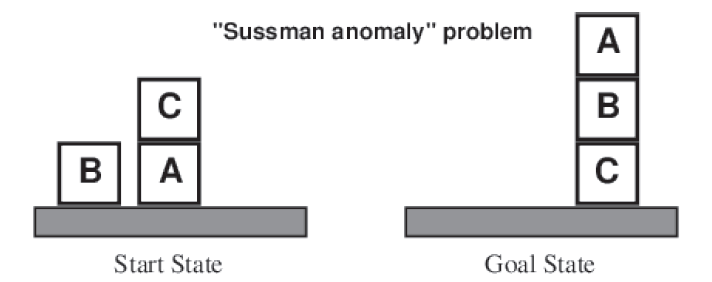
\includegraphics[width=\linewidth]{images/sussman.png}
\end{minipage}
\hfill
\begin{minipage}[c]{0.55\linewidth}
\centering
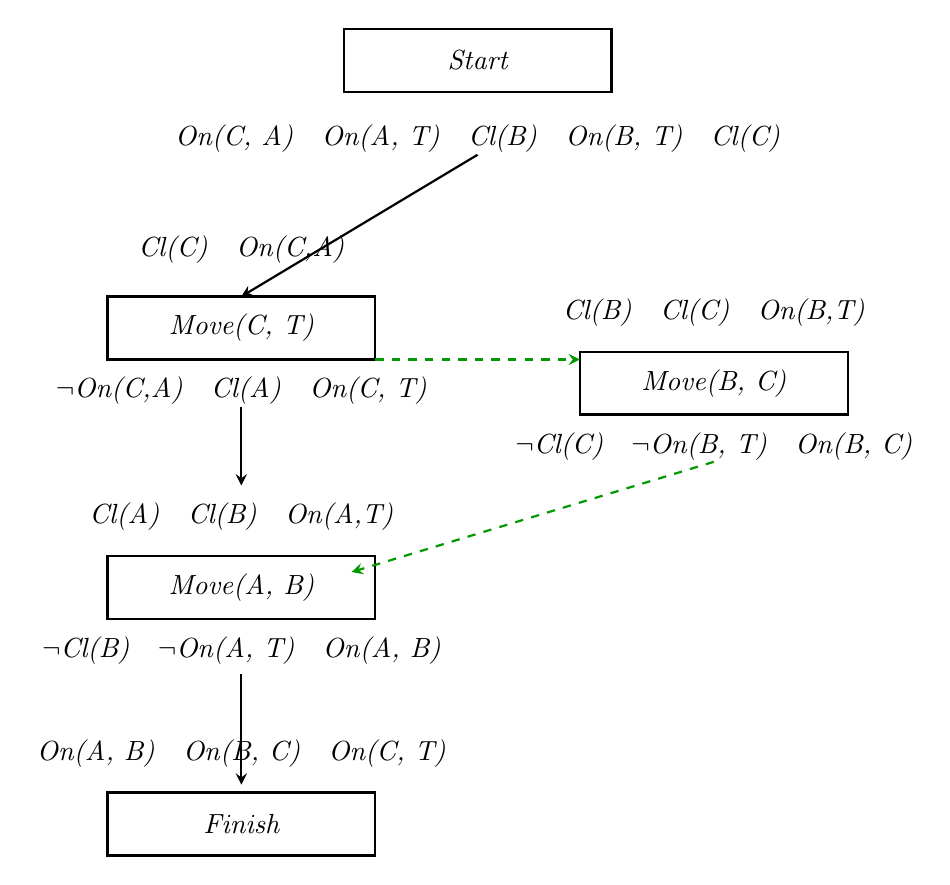
\begin{tikzpicture}[font=\itshape, >=stealth, thick]

\tikzset{
  action/.style={draw, rectangle, minimum width=34mm, minimum height=8mm, align=center},
  state/.style={align=center},
  darr/.style={->, dashed, green!60!black}
}

% Start
\node[action] (start) at (0,8) {Start};
\node[state] at (0,7) {On(C, A)\quad On(A, T)\quad Cl(B)\quad On(B, T)\quad Cl(C)};

% Move C T
\node[state]  at (-3,5.6) {Cl(C)\quad On(C,A)};
\node[action] (mCT) at (-3,4.6) {Move(C, T)};
\node[state]  at (-3,3.8) {$\neg$On(C,A)\quad Cl(A)\quad On(C, T)};

\draw[->] (0,6.8) -- (-3,5);

% Move B C
\node[state]  at (3,4.8) {Cl(B)\quad Cl(C)\quad On(B,T)};
\node[action] (mBC) at (3,3.9) {Move(B, C)};
\node[state]  at (3,3.1) {$\neg$Cl(C)\quad $\neg$On(B, T)\quad On(B, C)};

\draw[darr] (-1.3,4.2) -- (1.3,4.2);

% Move A B
\node[state]  at (-3,2.2) {Cl(A)\quad Cl(B)\quad On(A,T)};
\node[action] (mAB) at (-3,1.3) {Move(A, B)};
\node[state]  at (-3,0.5) {$\neg$Cl(B)\quad $\neg$On(A, T)\quad On(A, B)};

\draw[->] (-3,3.6) -- (-3,2.6);
\draw[darr] (3,2.9) -- (-1.6,1.5);

% Finish
\node[state]  at (-3,-0.8) {On(A, B)\quad On(B, C)\quad On(C, T)};
\node[action] (finish) at (-3,-1.7) {Finish};

\draw[->] (-3,0.2) -- (-3,-1.2);

\end{tikzpicture}
\end{minipage}

\end{figure}



\definition{Heuristic}{
Let $\Pi := \tuple{\mathcal{F}, \mathcal{A}, \mathcal{I}, \mathcal{G}}$ be a \linkterm{STRIPS task}{strips_task} and $\Theta_{\Pi} := \tuple{\mathcal{S}_{\Pi}, \mathcal{A}_{\Pi}, \mathcal{T}_{\Pi}, \mathcal{I}_{\Pi}, \mathcal{G}_{\Pi}}$ is the induced \linkterm{search problem}{search_problem}, A \textbf{heuristic function} or \textbf{heuristic} for $\Pi$ is a \linkterm{function}{function} $\func{h}{\mathcal{S}_{\Pi}}{\N \cup \set{\infty}}$ so that $h(s) = 0$ whenever $s \in \mathcal{G}_{\Pi}$
}{heuristic_strips}

\commandnote{
We use $\N$ (unlike \Defref{heuristic_function} where we used $\R^{+}_0$) because actions are discrete and we assume unit cost of $1$ (we are just counting steps now)
}

\definition{Perfect Heuristic}{
Let $\Pi := \tuple{\mathcal{F}, \mathcal{A}, \mathcal{I}, \mathcal{G}}$ be a \linkterm{STRIPS task}{strips_task} and $\Theta_{\Pi} := \tuple{\mathcal{S}_{\Pi}, \mathcal{A}_{\Pi}, \mathcal{T}_{\Pi}, \mathcal{I}_{\Pi}, \mathcal{G}_{\Pi}}$ is the induced \linkterm{search problem}{search_problem}, the \textbf{perfect heuristic} $h^{*}$ assigns every $s \in \mathcal{S}_{\Pi}$ the length of the shortest path from $s$ to a goal state $g \in \mathcal{G}_{\Pi}$, or $\infty$ if no such path exists.
}{perfect_heuristic_strips}

\commandnote{
Different from \Defref{goal_distance_function} (cost vs length)
}

\definition{Admissible}{
A \linkterm{heuristic}{heuristic_strips} $h$ for a \linkterm{STRIPS task}{strips_task} $\Pi$ is \textbf{admissible} if $h(s) \leq h^{*}(s) \quad \forall s \in \mathcal{S}_{\Pi}$
}{admissible_heuristic_strips}

\definition{Relaxed Planning Task}{
Let $\Pi$ be a \linkterm{STRIPS task}{strips_task}. A \textbf{relaxed planning task} $\Pi'$ is a modification of $\Pi$ such that the \linkterm{set}{def:set} of possible \linkterm{plans}{strips_plan} for $\Pi$ is a \linkterm{subset}{subset} of the \linkterm{set}{def:set} of possible \linkterm{plans}{strips_plan} for $\Pi'$.
}{relaxed_planning_task}

\definition{Relaxed Heuristic}{
A \textbf{relaxed heuristic} $h'$ for a \linkterm{STRIPS task}{strips_task} $\Pi$ is the \linkterm{perfect heuristic}{perfect_heuristic_strips} of an associated \linkterm{relaxed planning task}{relaxed_planning_task} $\Pi'$. That is:
\[
h(s) = h^{*}_{\Pi'}(s)
\]
}{relaxed_heuristic_strips}

\commandnote{
By definition, any solution to the original task $\Pi$ remains a valid solution in the relaxed task $\Pi'$. Because $\Pi'$ is "easier" (less constrained), its \linkterm{perfect heuristic}{perfect_heuristic_strips} value $h^{*}_{\Pi'}$ provides a lower bound on the true length $h^{*}$, ensuring that \linkterm{relaxed heuristics}{relaxed_heuristic_strips} are always \linkterm{admissible}{admissible_heuristic_strips}.
}

\definition{Only-Adds Relaxation}{
We drop $\text{pre}_a$ and $\text{del}_a$ for all $a \in \mathcal{A}$ resulting in a \linkterm{relaxed planning task}{relaxed_planning_task} where an action is just $a := \tuple{\text{add}_a}$
}{only_adds_strips}

\commandnote{
\textbf{Example: }Consider a goal $G := \{p, q\}$ and an action $a$ that adds $p, q$ but requires $r$. In the original task, I must first find a way to achieve $r$. In the \linkterm{only-adds relaxation}{only_adds_strips}, I can apply $a$ immediately in the initial state to reach the goal in a single step, because the requirement $r$ has been dropped.
}

\textbf{ATTENTION! }Search uses the real (un-relaxed) $\Pi$. The relaxation is applied \textbf{only} within the call to $h(s)$

\definition{Delete Relaxation}{
Let $\Pi := \tuple{\mathcal{F}, \mathcal{A}, \mathcal{I}, \mathcal{G}}$ be a \linkterm{STRIPS task}{strips_task}, the \textbf{delete relaxation} of $\Pi$ is the task $\Pi^{+} := \tuple{\mathcal{F}, \mathcal{A}^{+}, \mathcal{I}, \mathcal{G}}$ where $\mathcal{A}^{+} := \set{a^{+} \mid a \in \mathcal{A}}$ with $\text{pre}_{a^{+}} := \text{pre}_a$, and $\text{add}_{a^{+}} := \text{add}_a$, and $\text{del}_{a^{+}} := \emptyset$
}{delete_relaxation}


\definition{Relaxed Plan}{
Let $\Pi := \tuple{\mathcal{F}, \mathcal{A}, \mathcal{I}, \mathcal{G}}$ be a \linkterm{STRIPS task}{strips_task} and $\Theta_{\Pi} := \tuple{\mathcal{S}_{\Pi}, \mathcal{A}_{\Pi}, \mathcal{T}_{\Pi}, \mathcal{I}_{\Pi}, \mathcal{G}_{\Pi}}$ is the induced \linkterm{search problem}{search_problem}. A \textbf{relaxed plan} for a state $s \in \mathcal{S}_{\Pi}$ is a plan for $\tuple{\mathcal{F}, \mathcal{A}, s, \mathcal{G}}^{+}$. A \textbf{relaxed plan} for $\mathcal{I}$ is called a \textbf{relaxed plan} for $\Pi$
}{relaxed_plan}

\commandnote{
Relaxation is often used to mean \linkterm{delete relaxation}{delete_relaxation} by default
}

\definition{Relaxed Plan Existence Problem}{
By $\text{PlanEx}^{+}$, we denote the problem of deciding, given a \linkterm{STRIPS task}{strips_task} $\Pi := \tuple{\mathcal{F}, \mathcal{A}, \mathcal{I}, \mathcal{G}}$, whether or not there exists a \linkterm{relaxed plan}{relaxed_plan} for $\Pi$.
}{planex}

\commandnote{
This is easier than $\text{PlanEx}$ for general \linkterm{STRIPS}{strips}. \Algref{alg:planex} decides \linkterm{$\text{PlanEx}^{+}$}{planex}. The algorithm terminates after at most $\abs{\mathcal{F}}$ iterations, and thus runs in polynomial time (\linkterm{$\text{PlanEx}^{+}$}{planex} is in $\textsf{P}$).
}

\begin{algorithm}[H]
\caption{Deciding \linkterm{$\text{PlanEx}^{+}$}{planex} (Relaxed Plan Existence)}
\label{alg:planex}
\begin{algorithmic}[1]
\State \textbf{var} $F := I$
\While{$G \not\subseteq F$}
    \State $F' := F \cup \bigcup_{a \in A : \text{pre}_a \subseteq F} \text{add}_a$
    \If{$F' = F$} 
        \State \Return ``unsolvable''
    \EndIf
    \State $F := F'$
\EndWhile
\State \Return ``solvable''
\end{algorithmic}
\end{algorithm}

\definition{Optimal Relaxed Plan}{
Let $\Pi := \tuple{\mathcal{F}, \mathcal{A}, \mathcal{I}, \mathcal{G}}$ be a \linkterm{STRIPS task}{strips_task} and $\Theta_{\Pi} := \tuple{\mathcal{S}_{\Pi}, \mathcal{A}_{\Pi}, \mathcal{T}_{\Pi}, \mathcal{I}_{\Pi}, \mathcal{G}_{\Pi}}$ is the induced \linkterm{search problem}{search_problem}. An \textbf{optimal relaxed plan} for a state $s \in \mathcal{S}_{\Pi}$ is an optimal plan for $\tuple{\mathcal{F}, \mathcal{A}, \set{s}, \mathcal{G}}^{+}$.
}{optimal_relaxed_plan}

\definition{$h^{+}$}{
Let $\Pi := \tuple{\mathcal{F}, \mathcal{A}, \mathcal{I}, \mathcal{G}}$ be a \linkterm{STRIPS task}{strips_task} and $\Theta_{\Pi} := \tuple{\mathcal{S}_{\Pi}, \mathcal{A}_{\Pi}, \mathcal{T}_{\Pi}, \mathcal{I}_{\Pi}, \mathcal{G}_{\Pi}}$ is the induced \linkterm{search problem}{search_problem}. The \textbf{ideal delete relaxation heuristic} $h^{+}$ for $\Pi$ is a \linkterm{function}{function} $\func{h^{+}}{\mathcal{S}_{\Pi}}{\N \cup \set{\infty}}$ where for any $s \in \mathcal{S}_{\Pi}$, $h^{+}(s)$ is the length of an \linkterm{optimal relaxed plan}{optimal_relaxed_plan} for $s$ if a \linkterm{relaxed plan}{relaxed_plan} for $s$ exists. $h^{+}(s) = \infty$ otherwise.
}{h_plus}

\Lemma{
Let $\Pi := \tuple{\mathcal{F}, \mathcal{A}, \mathcal{I}, \mathcal{G}}$ be a \linkterm{STRIPS task}{strips_task} and $\Theta_{\Pi} := \tuple{\mathcal{S}_{\Pi}, \mathcal{A}_{\Pi}, \mathcal{T}_{\Pi}, \mathcal{I}_{\Pi}, \mathcal{G}_{\Pi}}$ is the induced \linkterm{search problem}{search_problem}. For a state $s \in \mathcal{S}_{\Pi}$, if $\tuple{a_1, \cdots, a_n}$ is a \linkterm{plan}{strips_plan} for $\Pi_s := \tuple{\mathcal{F}, \mathcal{A}, \set{s}, \mathcal{G}}$, then $\tuple{a^{+}_1, \cdots, a^{+}_n}$ is a \linkterm{plan}{strips_plan} for $\Pi^{+}$
}{}

\Theorem{
\linkterm{$h^{+}$}{h_plus} is \linkterm{admissible}{admissible_heuristic_strips}.
}{}

\newpage
\minititle{Example}
Consider the following \linkterm{STRIPS task}{strips_task} $\Pi := \tuple{\mathcal{F}, \mathcal{A}, \mathcal{I}, \mathcal{G}}$:
\begin{itemize}
\item $\mathcal{F} := \set{\text{truck}(x) \mid x \in \set{A,B,C,D}} \cup \set{\text{pack}(x)\mid x \in \set{A,B,C,D,T}}$ 

i.e. we are representing where is the truck via $\text{truck}(x)$ and where is the pack via $\text{pack}(x)$ where $\text{pack}(T)$ means the packet is in the truck

\item $\mathcal{I} := \set{\text{truck}(A), \text{pack}(C)}$ \hfill initially, the truck is at $A$ and the packet is at $C$
\item $\mathcal{G} := \set{\text{truck}(A), \text{pack}(D)}$ \hfill we want to move the packet to $D$ and go back to $A$
\item $\mathcal{A} \leadsto$ we write action $a := \tuple{\text{pre}_a, \text{add}_a, \text{del}_a}$ as $a := \text{pre}_a \Rightarrow \text{add}_a , \neg \text{del}_a$
\begin{itemize}
    \item $\text{drive}(x,y) := \text{truck}(x) \Rightarrow \text{truck}(y) , \neg \text{truck}(x)$
    \item $\text{load}(x) := \text{truck}(x), \text{pack}(x) \Rightarrow \text{pack}(T), \neg \text{pack}(x)$
    \item $\text{unload}(x) := \text{truck}(x), \text{pack}(T) \Rightarrow \text{pack}(x), \neg \text{pack}(T)$
\end{itemize}
\item Relaxed Actions:
\begin{itemize}
    \item $\text{drive}(x,y) := \text{truck}(x) \Rightarrow \text{truck}(y)$
    \item $\text{load}(x) := \text{truck}(x), \text{pack}(x) \Rightarrow \text{pack}(T)$
    \item $\text{unload}(x) := \text{truck}(x), \text{pack}(T) \Rightarrow \text{pack}(x)$
\end{itemize}
\end{itemize}

For convenience: 
\begin{itemize}
    \item we represent a state $\text{truck}(X), \text{pack}(Y)$ by writing $XY$
    \item actions are shortened to $drXY,loX, ulX$
\end{itemize}

Let's see how to relax during search:

Initially, we are in the real problem in the initial state $AC$ and the goal is $AD$. 
\begin{figure}[H]
    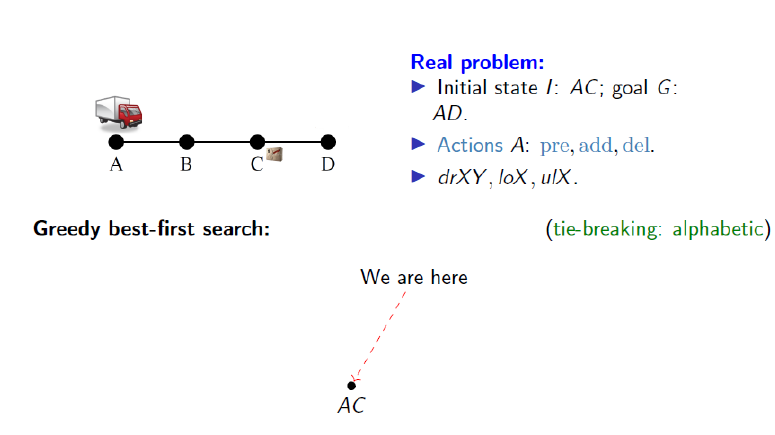
\includegraphics[width=0.5\linewidth]{images/p1.png}
\end{figure}

We go the relaxed world to calculate \linkterm{$h^{+}$}{h_plus} of the current state. We see that we would reach the goal if we apply

$\tuple{drAB, drBC, loC, drCD, ulD}$ (we do not need to go back to $A$, since no deletions, we are still there). So $\linkterm{h^{+}}{h_plus}(AC) = \abs{\tuple{drAB, drBC, loC, drCD, ulD}} = 5$

\begin{figure}[H]
    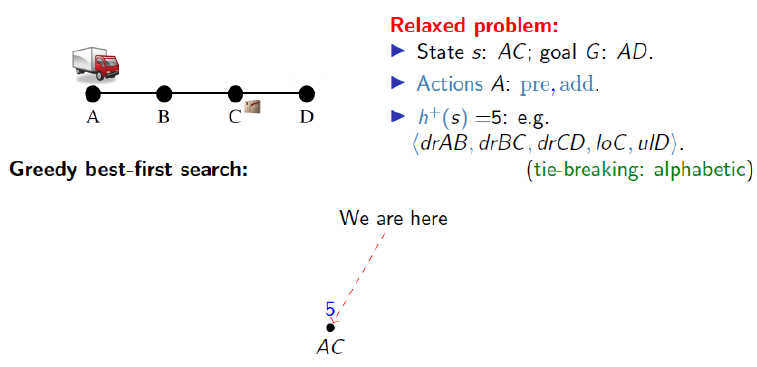
\includegraphics[width=0.5\linewidth]{images/p2.png}
\end{figure}

We go back to the real problem, we know the only action we can take is $drAB$ (the only possible successor state is $BC$), so we go there:
\begin{figure}[H]
    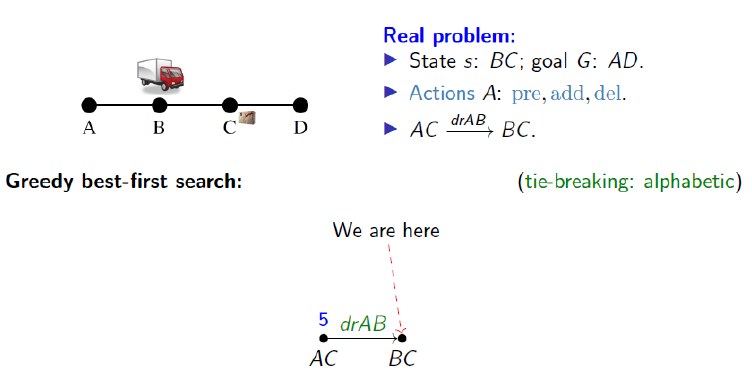
\includegraphics[width=0.5\linewidth]{images/p3.png}
\end{figure}

We go the relaxed world to calculate $\linkterm{h^{+}}{h_plus}(BC)$. We see that we would reach the goal if we apply $\tuple{drBC, loC, drCD, ulD, drBA}$, so $\linkterm{h^{+}}{h_plus}(BC)=5$
\begin{figure}[H]
    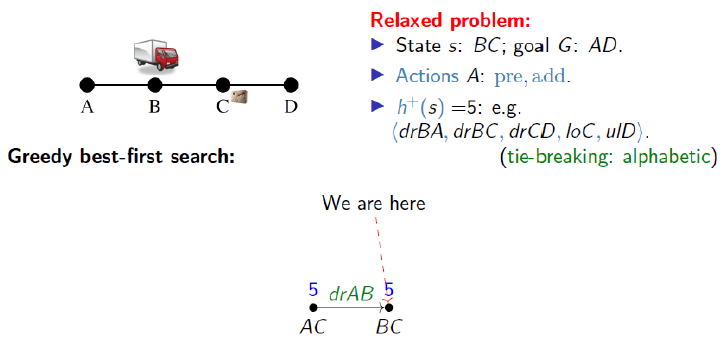
\includegraphics[width=0.5\linewidth]{images/p4.png}
\end{figure}

we go back to the real world, we know that two actions are applicable $drBA, drBC$ (two possible successor states: $AC, CC$). 
\begin{itemize}
    \item we go first to $CC$:
\begin{figure}[H]
    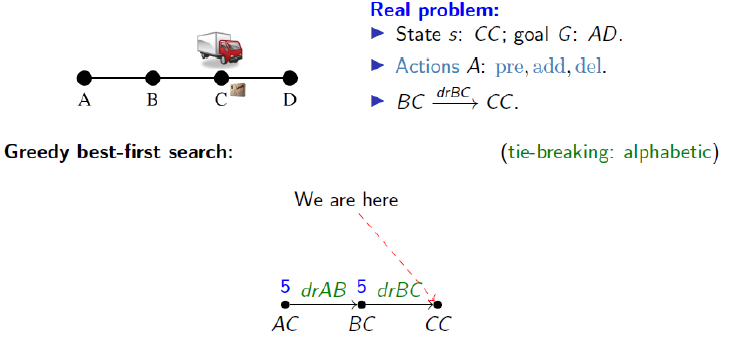
\includegraphics[width=0.5\linewidth]{images/p5.png}
\end{figure}

we go to the relaxed world to calculate $\linkterm{h^{+}}{h_plus}(CC)$:
\begin{figure}[H]
    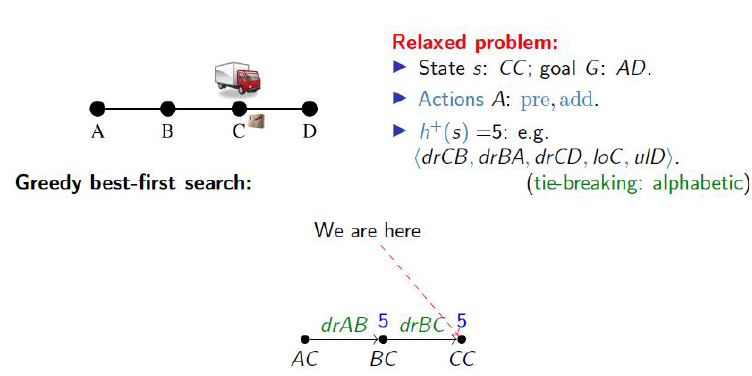
\includegraphics[width=0.5\linewidth]{images/p6.png}
\end{figure}

\item next we go to $AC$, we figure that it has been explored, hence we mark it as duplicate:
\begin{figure}[H]
    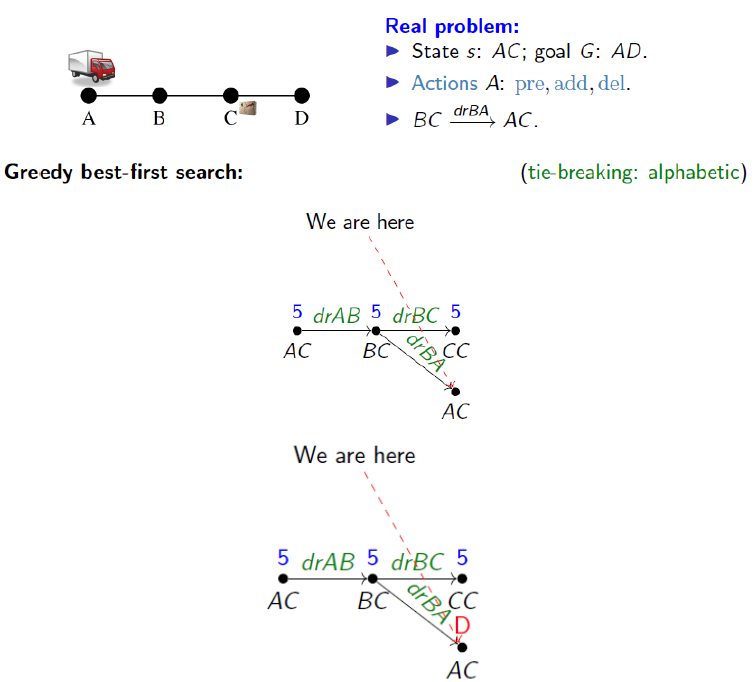
\includegraphics[width=0.5\linewidth]{images/p7.png}
\end{figure}
\end{itemize}

Back to real, we are at $CC$, we have three possible successors, we can move to $D$ ($DC$), we can unload ($CT$), we can move to $B$ ($BC$)
\begin{itemize}
\item Let's see $DC$:
\begin{figure}[H]
    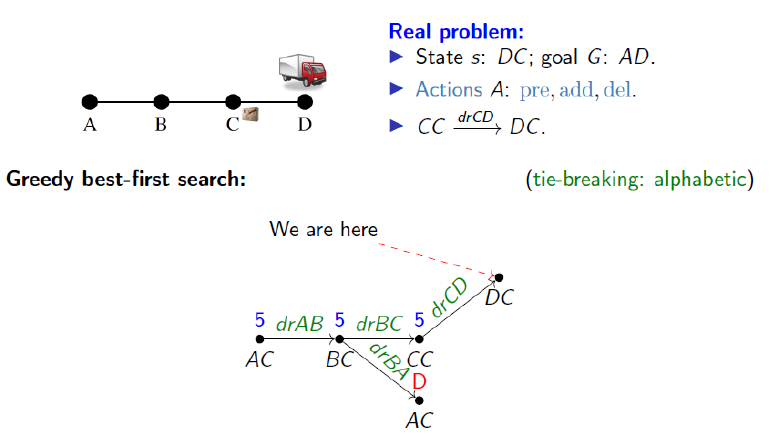
\includegraphics[width=0.5\linewidth]{images/p8.png}
\end{figure}

We relax to calculate:
\begin{figure}[H]
    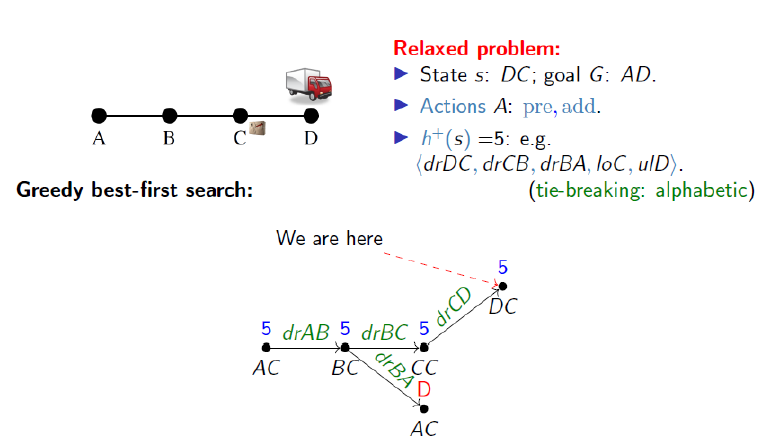
\includegraphics[width=0.5\linewidth]{images/p9.png}
\end{figure}
\item Let's see $CT$:
\begin{figure}[H]
    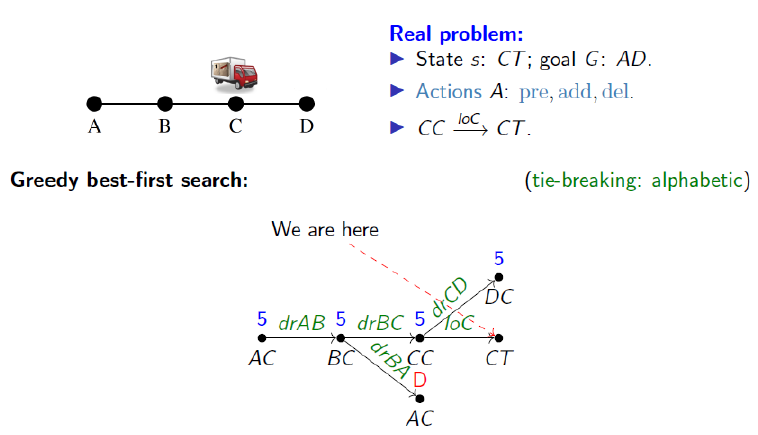
\includegraphics[width=0.5\linewidth]{images/p10.png}
\end{figure}

We relax to calculate: notice that $\linkterm{h^{+}}{h_plus}(CT)=4$ because we can do $drCD, ulD, drCB, drBA$
\begin{figure}[H]
    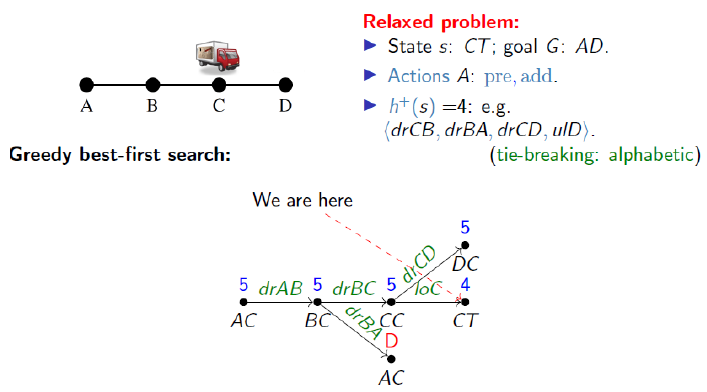
\includegraphics[width=0.5\linewidth]{images/p11.png}
\end{figure}
\item Let's see $BC$: we mark as duplicate
\end{itemize}

Next we can expand $CT$ with \linkterm{$h^{+}$}{h_plus} of 4 or $DC$ with \linkterm{$h^{+}$}{h_plus} of 5. We choose $CT$. From there, we have three successors: we can unload ($CC$, duplicate), we can move to $D$ ($DT$), we can move to $B$ ($BT$), we relax to calculate \linkterm{$h^{+}$}{h_plus} of each:
\begin{figure}[H]
    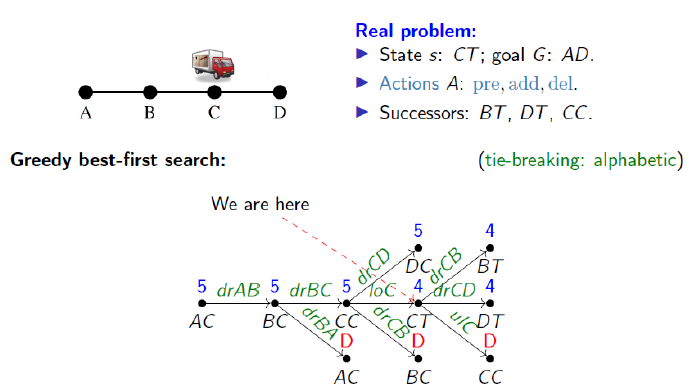
\includegraphics[width=0.5\linewidth]{images/p12.png}
\end{figure}

We expand next $BT$ (break ties alphabetically), from there we can unload ($BB$), we can move to $A$ ($AT$), we can move to $C$ ($CT$, duplicate). We calculate \linkterm{$h^{+}$}{h_plus} of each:

\begin{figure}[H]
    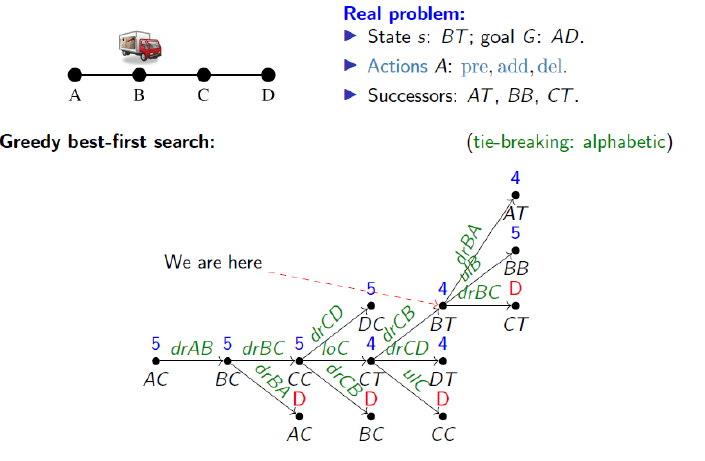
\includegraphics[width=0.5\linewidth]{images/p13.png}
\end{figure}

We expand $AT$ first, we have two successors, we can move to $B$ ($BT$, duplicate), or we can unload $(AA)$:
\begin{figure}[H]
    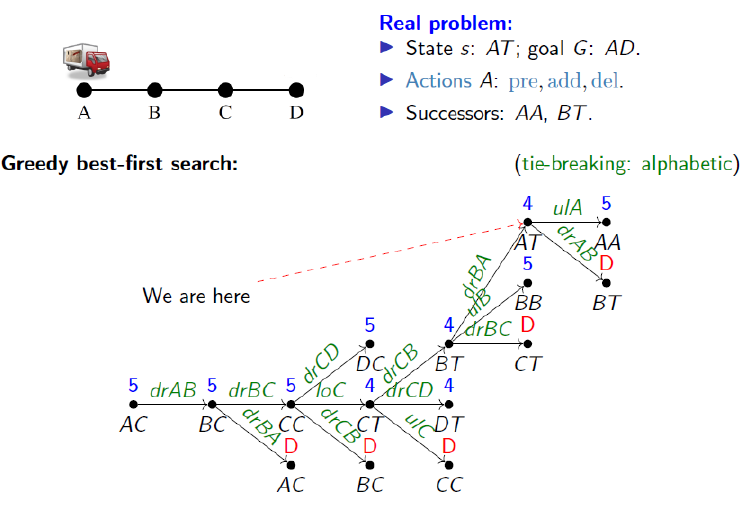
\includegraphics[width=0.5\linewidth]{images/p14.png}
\end{figure}

We can expand next $AA$ or $BB$ with \linkterm{$h^{+}$}{h_plus} of 5 or expand $DT$ with \linkterm{$h^{+}$}{h_plus} of 4 (remember when we expanded $CT$ we had two successors to investigate, $BT$ and $DT$ and we broke ties alphabetically). We choose to expand $DT$:
\begin{figure}[H]
    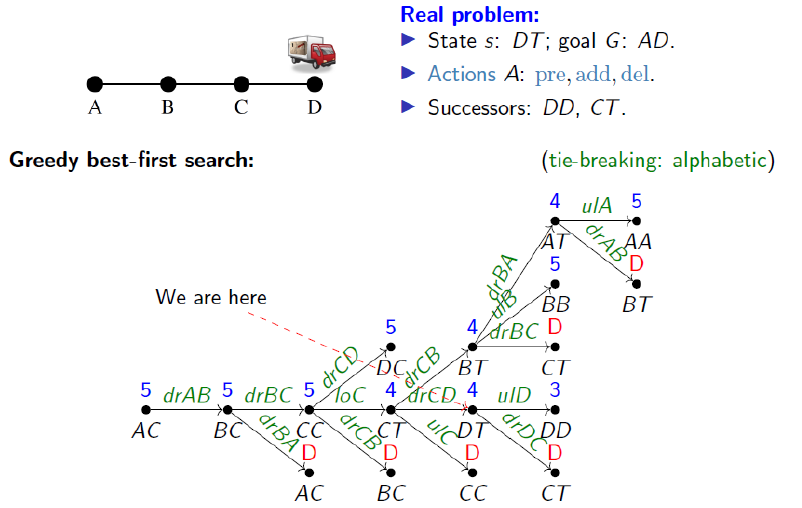
\includegraphics[width=0.5\linewidth]{images/p15.png}
\end{figure}

We expand next $DD$, $CD$, and $BD$ respectively:

\begin{figure}[H]
\centering
\begin{minipage}{0.32\linewidth}
\centering
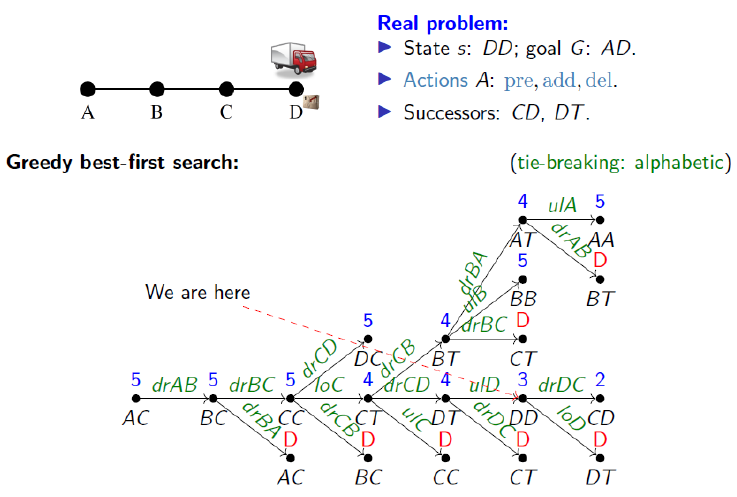
\includegraphics[width=\linewidth]{images/p16.png}
\end{minipage}
\hfill
\begin{minipage}{0.32\linewidth}
\centering
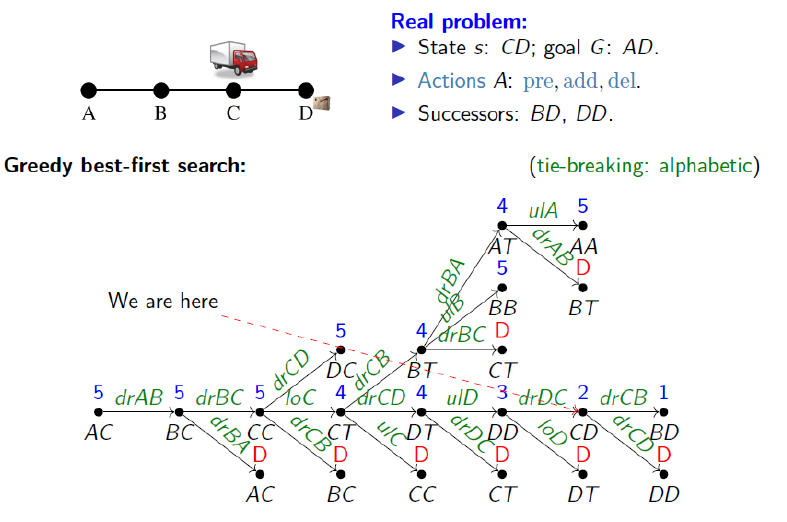
\includegraphics[width=\linewidth]{images/p17.png}
\end{minipage}
\hfill
\begin{minipage}{0.32\linewidth}
\centering
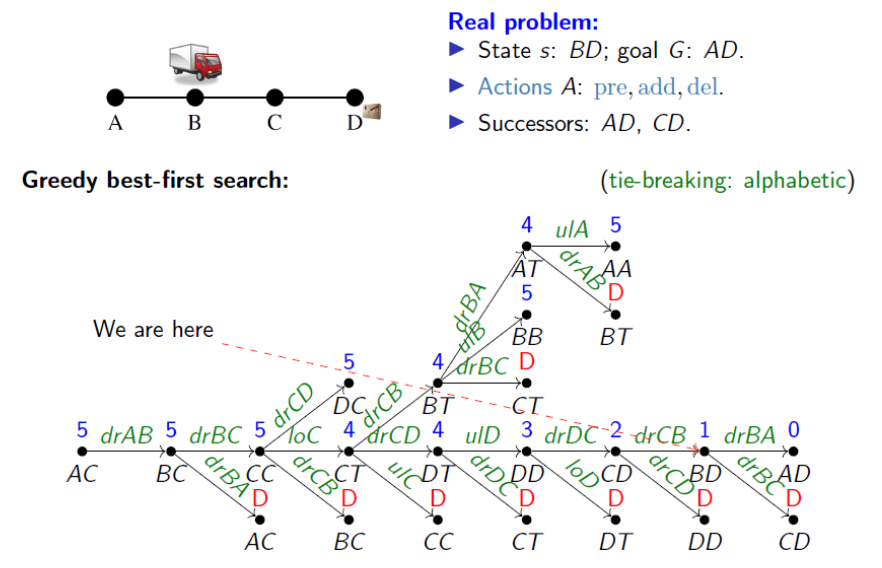
\includegraphics[width=\linewidth]{images/p18.png}
\end{minipage}
\end{figure}

We go to $AD$ only to figure out that this is a goal state! (Truck at A, pack at D). 
\begin{figure}[H]
    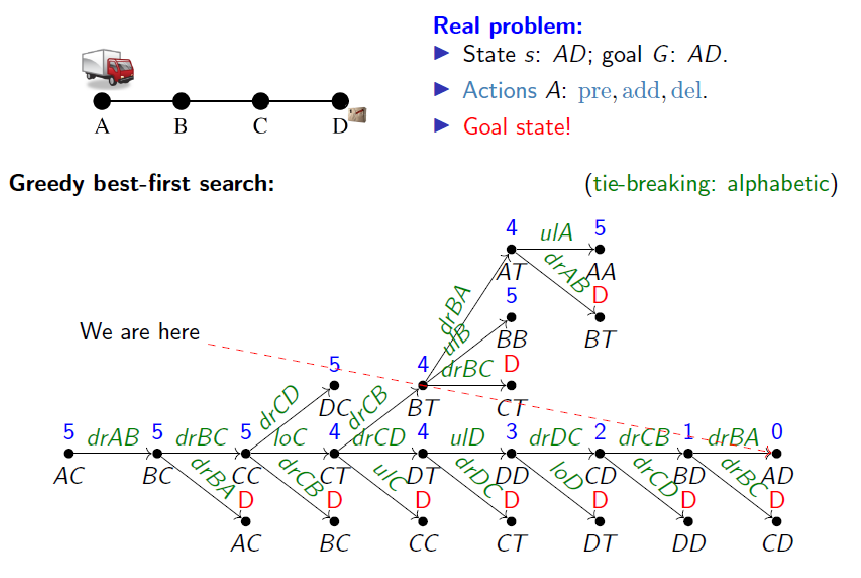
\includegraphics[width=0.5\linewidth]{images/p19.png}
\end{figure}

To sum up the steps that we found:
\[
\text{drive}(A,B) \leadsto \text{drive}(B,C) \leadsto \text{load}(C) \leadsto \text{drive}(C,D) \leadsto \text{unload}(D) \leadsto \text{drive}(D,C) \leadsto \text{drive}(C,B) \leadsto \text{drive}(B,A)
\]




\printbibliography
\end{document}
